\documentclass[14pt,a4paper]{extarticle}
\usepackage{fontspec}
\setmainfont{Times New Roman}
\setsansfont{Arial}
\setmonofont{Consolas}
\usepackage{polyglossia}
\setdefaultlanguage{russian}
\setotherlanguage{english}
\usepackage[left=30mm,right=15mm,top=20mm,bottom=20mm]{geometry}
\usepackage{setspace}
\onehalfspacing
\usepackage{titlesec}
\titleformat{\section}{\normalfont\fontsize{16}{20}\selectfont\bfseries}{\thesection.}{0.6em}{}
\titleformat{\subsection}{\normalfont\fontsize{14}{18}\selectfont\bfseries}{\thesubsection.}{0.6em}{}
\titlespacing*{\section}{0pt}{0pt}{12pt}
\titlespacing*{\subsection}{0pt}{14pt}{8pt}
\usepackage{graphicx}
\usepackage{caption}
\captionsetup{font=small,labelfont=normalfont,labelsep=endash,justification=raggedright,singlelinecheck=false}
\usepackage{longtable,array,ragged2e}
\usepackage{etoolbox}
\makeatletter
% В новых ядрах LaTeX бесконечное сжатие мешает разбиению страниц longtable.
\patchcmd{\LT@output}{\vss}{\vfil}{}{}
\patchcmd{\LT@output}{\vss}{\vfil}{}{}
\makeatother
\newlength{\tablecontentwidth}
\setlength{\tabcolsep}{4pt}
\renewcommand{\arraystretch}{1.15}
\setlength{\LTpre}{8pt}
\setlength{\LTpost}{8pt}
\usepackage{enumitem}
\setlist{nosep,topsep=6pt,leftmargin=12.5mm}
\usepackage{placeins}
\usepackage{needspace}
\usepackage{xurl}
\usepackage[unicode,hidelinks,bookmarksnumbered]{hyperref}
\hypersetup{pdftitle={ИС «Потеряшки». Этапы 1–2},pdfauthor={Шубин Егор Вячеславович; Евграфов Артём Андреевич}}
\urlstyle{same}
\setcounter{tocdepth}{2}
\setlength{\parindent}{12.5mm}
\setlength{\parskip}{0pt}
\setlength{\emergencystretch}{3em}
\clubpenalty=10000
\widowpenalty=10000
\displaywidowpenalty=10000
\raggedbottom

\usepackage{fvextra}
\graphicspath{{../part1/}{../part2/}}
\begin{document}
\begin{titlepage}
\begin{center}
{\fontsize{18}{22}\selectfont Университет ИТМО\par}
\vspace{8mm}
{\fontsize{16}{20}\selectfont Факультет программной инженерии и компьютерной техники\par
Образовательная программа\par
«Системное и прикладное программное обеспечение»\par}
\vspace{30mm}
{\fontsize{16}{22}\selectfont\bfseries Курсовая работа\par
По дисциплине «Информационные системы»\par}
\vspace{10mm}
{\fontsize{16}{22}\selectfont\bfseries Информационная система для поиска\par
и возврата потерянных вещей «Потеряшки»\par}
\vspace{8mm}
{\fontsize{16}{20}\selectfont Этапы 1–2\par}
\end{center}
\vspace{20mm}
\begin{flushright}
Выполнили студенты группы P3309\\
Шубин Егор Вячеславович\\
Евграфов Артём Андреевич\\
\vspace{7mm}
Проверил:\\
Николаев Владимир Вячеславович
\end{flushright}
\vfill
\begin{center}
Санкт-Петербург 2026
\end{center}
\end{titlepage}

\pagenumbering{arabic}
\tableofcontents
\clearpage

\clearpage
\section*{Задание}
\phantomsection
\addcontentsline{toc}{section}{Задание}

Отчёт по первому этапу курсовой работы: анализ предметной области и проектирование системы.

Первый этап курсовой работы включает:

\begin{enumerate}
\item Выбор предметной области информационной системы.
\item Подробное текстовое описание предметной области.
\item Обоснование назначения системы и решаемых задач.
\item Формулирование функциональных и нефункциональных требований.
\item Построение моделей основных прецедентов и описание их сценариев.
\item Выбор архитектуры, технологий и фреймворков с учётом демонстрации на helios.
\item Подготовку отчёта.
\end{enumerate}

\clearpage
\section{Предметная область}

Предметная область — поиск и возврат потерянных вещей в городской среде. Разрабатываемая информационная система «Потеряшки» предназначена для публикации объявлений о потерянных и найденных предметах с указанием места и времени события, поиска совпадений, проверки заявителей и фиксации возврата. Дополнительно предусматриваются справочная интеграция с Петербургским метрополитеном, доступ к пользовательским функциям по подписке и аукционы вещей, которыми продавец вправе распоряжаться.

В качестве начального региона выбран Санкт-Петербург. Приложение проектируется как адаптивное веб-приложение. Подписка предоставляет доступ к пользовательским операциям после верификации учётной записи. Регистрация, оплата, восстановление доступа и официальные инструкции доступны до активации подписки. Цена задаётся администратором; конкретная стоимость не является требованием этапа 1. Базовый расчётный период подписки — 30 суток без автоматического списания.

Для демонстрации оплаты используется тестовый платёжный адаптер. Проверка пользователя включает подтверждение электронной почты и рассмотрение профиля модератором. Паспортные данные при регистрации не запрашиваются. После безуспешного поиска владельца пользователь может подать заявку на аукцион; возможность продажи зависит от основания распоряжения вещью и решения по заявке.

\clearpage
\section{Подробное описание предметной области}

\FloatBarrier
\Needspace{6\baselineskip}
\subsection{Участники и их интересы}

Владелец потерянной вещи стремится быстро найти предмет и подтвердить своё право на его получение. Нашедший стремится сообщить о находке, передать её надлежащему получателю и избежать многократных необоснованных обращений. Один пользователь может выступать в обеих ролях в разных ситуациях. Покупатель участвует в аукционе; продавцом становится пользователь, право распоряжения вещью которого проверено.

Постоянные роли доступа — участник, модератор и администратор. Нашедший, владелец, продавец и покупатель обозначают положение участника в конкретном процессе. Модератор проверяет учётные записи, объявления, жалобы и документы для допуска аукционов. Администратор управляет полномочиями сотрудников, тарифами, справочником организаций и аудитом. Физическое хранение и выдачу вещей могут осуществлять пользователи либо сторонние организации: метрополитен, городское бюро находок, полиция. Эти организации не считаются зарегистрированными партнёрами без отдельной договорённости.

Платёжный сервис подтверждает результаты оплаты подписки. Пользователь обращается к нему через платёжную форму. Почтовый сервис доставляет ссылки подтверждения и восстановления доступа. В самой системе уведомления сохраняются независимо от успешности доставки письма.

\FloatBarrier
\Needspace{6\baselineskip}
\subsection{Существующий процесс и проблемы}

Сведения о находках обычно распределены между объявлениями в социальных сетях, локальными чатами, бюро находок и транспортными организациями. Объявления оформляются неодинаково: часто отсутствуют время, точное место, категория или актуальный статус. Потерявшему приходится повторять поиск на нескольких площадках и связываться с авторами уже неактуальных сообщений.

Нашедший не всегда знает порядок передачи вещи и нужную организацию. Публикация полной фотографии документов или всех отличительных признаков увеличивает вероятность злоупотреблений. Несколько претендентов могут одновременно заявить права на один предмет. Отсутствие истории решений затрудняет разбор споров, а свободная публикация без проверки повышает долю рекламы, ложных находок и повторяющихся сообщений.

Подписка повышает стоимость массового злоупотребления и поддерживает работу сервиса, но сама по себе не гарантирует добросовестность. Поэтому в проекте она дополняется верификацией профиля, предварительной модерацией, ограничением частоты действий и механизмом жалоб. Сроки подписки и судьба уже опубликованной находки управляются раздельно.

\FloatBarrier
\Needspace{6\baselineskip}
\subsection{Процесс работы с потерянными и найденными вещами}

Пользователь регистрируется, подтверждает почту, проходит проверку профиля и активирует подписку. Затем он создаёт объявление типа «Потерял» или «Нашёл». Для находки фиксируются предмет, категория, описание, место, дата и время обнаружения, текущее место хранения. Для потери допускается временной интервал и приблизительный район, поскольку точный момент может быть неизвестен.

Часть признаков является публичной: категория, цвет, общее описание, район, дата, безопасная фотография. Контрольные признаки — например, содержимое сумки или индивидуальная отметка — видны только автору и уполномоченному модератору. Контактные сведения и точный адрес хранения не публикуются в общем каталоге.

Объявление проходит модерацию. После публикации пользователи ищут предметы по типу объявления, категории, месту и времени. Поиск возвращает опубликованные карточки, соответствующие заданным условиям. Сходство описания не считается доказательством принадлежности: пользователь направляет заявку и описывает скрытые признаки. Автор находки рассматривает заявку, может запросить уточнения и согласовать передачу через внутренний диалог.

После согласования система резервирует находку за одним претендентом. Фактическая передача происходит вне приложения, затем обе стороны подтверждают её. До второго подтверждения вещь имеет статус «Передача ожидает подтверждения»; при споре дело передаётся модератору. Если предмет хранится у организации, система показывает её порядок выдачи; самостоятельное подтверждение в приложении не заменяет решения организации.

\FloatBarrier
\Needspace{6\baselineskip}
\subsection{Находки в метрополитене}

Для места типа «Метро» указываются город, станция и при наличии линия или участок поездки. В карточке показываются официальные инструкции: справочная Петербургского метрополитена 8-800-350-11-55; вещи передаются дежурному по станции и находятся в метро 10 дней, затем передаются в городской Центр утерянных документов и средств связи по адресу: ул. Большая Монетная, д. 16, офис-центр № 1. Для получения вещи требуется паспорт и заявление. Эти сведения взяты с официальной страницы метрополитена [1].

Найденную в метро вещь пользователь передаёт сотруднику станции и может опубликовать информационное объявление с указанием организации хранения. Приложение предлагает уточнить актуальные условия по официальному контакту. Десятидневный срок не используется как срок допуска к аукциону. Данные справочника содержат ссылку на источник, дату проверки и дату следующего пересмотра; администратор проверяет их не реже одного раза в 30 дней.

Интеграция с метрополитеном реализуется через справочник организаций: приложение подбирает контакты и инструкцию по выбранному месту. Пользователь обращается в организацию по указанному телефону или через официальный сайт. Прямой обмен сведениями о находках может быть добавлен при наличии доступного программного интерфейса и договорённости с метрополитеном.

\FloatBarrier
\Needspace{6\baselineskip}
\subsection{Условия аукциона}

Обычная находка не становится товаром только потому, что на объявление долго нет откликов. Статья 227 ГК РФ предусматривает уведомление известного владельца; находку в помещении или транспорте передают представителю владельца помещения или транспорта. Когда надлежащий получатель неизвестен, предусмотрено заявление в полицию либо орган местного самоуправления [3]. Публикация в «Потеряшках» не заменяет такого заявления.

Для обычной находки статья 228 ГК РФ связывает приобретение собственности с отсутствием установленного или заявившегося правообладателя в течение шести месяцев после заявления о находке в компетентный орган. При отказе нашедшего приобрести вещь она поступает в муниципальную собственность [4]. Поэтому проект использует дату официального заявления и проверку подтверждающих материалов, а не дату публикации объявления.

Продавец подаёт заявку на допуск вещи к аукциону, указывает основание распоряжения и прикладывает подтверждение обращения и права. Модератор проверяет комплектность, отсутствие открытого спора и принадлежность допустимой категории; сомнительное основание ведёт к отказу. Автоматически подтверждается только комплектность данных, решение о допуске принимает модератор. Вещи, переданные метро или иной организации, обычный пользователь на аукцион не выставляет.

Из аукционного каталога исключаются документы, банковские карты, предметы с персональными данными, опасные и запрещённые предметы, а также вещи с неразрешёнными заявлениями владельцев. Для электронных устройств требуется подтверждение законного распоряжения и удаления пользовательских данных. Частные случаи продажи скоропортящихся вещей не включены в учебный процесс.

Аукцион проводится на повышение: задаются стартовая цена, шаг и время начала и окончания. Продавец не может делать ставки на собственный лот. Победителем становится автор наибольшей принятой ставки до срока окончания. Отсутствие ставок означает завершение без победителя. Расчёты за лот и доставку стороны организуют самостоятельно; система фиксирует договорённость и подтверждение передачи.

\FloatBarrier
\Needspace{6\baselineskip}
\subsection{Основные информационные объекты}

\begingroup
\setstretch{1}
\fontsize{12}{14}\selectfont
\setlength{\tablecontentwidth}{\dimexpr\linewidth-6\tabcolsep-4\arrayrulewidth\relax}
\begin{longtable}{|>{\RaggedRight\arraybackslash}p{0.28\tablecontentwidth}|>{\RaggedRight\arraybackslash}p{0.32\tablecontentwidth}|>{\RaggedRight\arraybackslash}p{0.40\tablecontentwidth}|}
\caption{Основные информационные объекты}\label{tab:1}\\
\hline
\textbf{Объект} & \textbf{Основные сведения} & \textbf{Назначение} \\ \hline
\endfirsthead
\multicolumn{3}{r}{\footnotesize Продолжение таблицы \thetable} \\
\hline
\textbf{Объект} & \textbf{Основные сведения} & \textbf{Назначение} \\ \hline
\endhead
\multicolumn{3}{r}{\footnotesize Продолжение на следующей странице} \\
\endfoot
\endlastfoot
Пользователь & ID, имя, email, хеш пароля, набор ролей, статус проверки и блокировки, версия токенов & Учёт участника и управление доступом \\ \hline
Токен обновления & Пользователь, хеш токена, срок действия, отметка отзыва & Обновление доступа и завершение авторизации \\ \hline
Верификация & Пользователь, дата подачи, решение, причина, модератор & История рассмотрения профиля \\ \hline
Подписка & Пользователь, начало и окончание, статус, оплаченный тариф & Проверка права доступа \\ \hline
Платёж & ID операции, сумма, статус, внешний идентификатор & Связь оплаты с подпиской \\ \hline
Объявление & Тип, автор, категория, описание, время, место, статус & Учёт потери или находки \\ \hline
Фотография & Объявление, ключ файла, MIME, размер, доступность & Безопасная иллюстрация предмета \\ \hline
Контрольный признак & Объявление, закрытое описание & Проверка претендента \\ \hline
Место & Город, тип, район/\allowbreak{}адрес, станция, координаты при наличии & Поиск и подбор организации \\ \hline
Организация & Название, контакты, инструкция, URL источника, даты проверки & Справочная интеграция \\ \hline
Заявка на возврат & Находка, претендент, доказательства, статус & Рассмотрение права на получение \\ \hline
Диалог и сообщение & Участники, заявка, текст, время & Согласование возврата \\ \hline
Передача & Находка или лот, стороны, подтверждения, дата & Завершение жизненного цикла \\ \hline
Жалоба & Автор, объект, причина, решение & Контроль качества и спорные ситуации \\ \hline
Допуск к аукциону & Находка, основание, документы, решение & Контроль возможности продажи \\ \hline
Аукцион и ставка & Лот, продавец, цены, сроки, участник, серверное время & Организация торгов \\ \hline
Уведомление и аудит & Получатель/\allowbreak{}исполнитель, событие, время, результат & Информирование и прослеживаемость \\ \hline
\end{longtable}
\endgroup

Это концептуальный состав данных. Логическая и физическая схемы Postgre\allowbreak{}SQL разрабатываются на следующем этапе.

\FloatBarrier
\Needspace{6\baselineskip}
\subsection{Статусы и бизнес-правила}

Объявление проходит состояния «Черновик \ensuremath{\rightarrow} На модерации \ensuremath{\rightarrow} Опубликовано». Из модерации возможны «Отклонено» или «На исправлении»; изменённое объявление проходит повторную проверку. Опубликованная находка может перейти в «Зарезервировано \ensuremath{\rightarrow} Передача ожидает подтверждения \ensuremath{\rightarrow} Возвращено». Отмена согласования возвращает её в опубликованное состояние. Автор может закрыть поиск; модератор — скрыть нарушающее правила объявление. Закрытая находка сохраняется в истории и не участвует в выдаче активных результатов.

У аукциона состояния «Черновик \ensuremath{\rightarrow} На проверке \ensuremath{\rightarrow} Допущен \ensuremath{\rightarrow} Запланирован \ensuremath{\rightarrow} Активен \ensuremath{\rightarrow} Завершён с победителем /\allowbreak{} Завершён без ставок». Дополнительно предусмотрены «Отказано», «Приостановлен», «Отменён», «Передан покупателю». Неурегулированная претензия блокирует запуск и новые ставки; модератор определяет дальнейшее решение, оно сохраняется в аудите.

\begin{itemize}
\item BR-01. Публикация, поиск каталога, заявки, сообщения и ставки доступны проверенному, незаблокированному пользователю с активной подпиской. Сотрудники работают по служебным ролям без платной подписки.
\item BR-02. До подписки разрешены регистрация, подтверждение почты, проверка профиля, покупка или продление подписки, восстановление доступа, просмотр собственных статусов и официальных контактов.
\item BR-03. После истечения подписки новые пользовательские операции закрываются; ранее опубликованные объявления остаются видимыми. Участник может прочитать существующий диалог, подтвердить уже согласованную передачу, закрыть своё объявление и направить жалобу по своему делу без продления.
\item BR-04. Проверка профиля не подтверждает принадлежность конкретной вещи. Каждая заявка на возврат рассматривается отдельно. Оплата не отменяет модерацию.
\item BR-05. Для находки обязательны место и дата/\allowbreak{}время. Для потери допускается интервал; его начало не позже конца. Время события не может находиться в будущем. Ввод и отображение выполняются в часовом поясе Санкт-Петербурга Europe/\allowbreak{}Moscow; хранение и сравнение — как момент времени UTC.
\item BR-06. Для метро обязательна станция либо описание участка поездки. Приложение не обещает наличие вещи в реестре организации.
\item BR-07. У находки может быть несколько заявок, но не более одного действующего резервирования. Автор не направляет заявку на собственную находку.
\item BR-08. Возврат закрывается после двух подтверждений или мотивированного решения модератора. Скрытые признаки и материалы спора не входят в публичный каталог.
\item BR-09. Продление оплаченной подписки добавляет 30 суток от более позднего значения: текущего момента или окончания действующей подписки. Повторное платёжное событие не добавляет срок повторно.
\item BR-10. Блокировка запрещает действия независимо от подписки. Принятые до истечения подписки ставки сохраняются; блокировка участника активного аукциона приостанавливает его до решения модератора.
\item BR-11. Аукцион возможен только после отдельного допуска. Отсчёт шести месяцев по обычной находке ведётся от официального заявления; истечение срока лишь позволяет подать заявку на проверку и не создаёт допуск автоматически.
\item BR-12. Ставка принимается при активном аукционе и серверном времени строго раньше окончания. Минимальная ставка — стартовая цена при отсутствии ставок, иначе последняя принятая цена плюс шаг. Денежные суммы хранятся точно, без float.
\item BR-13. Одновременные ставки обрабатываются последовательно в транзакции для одного лота. При одинаковом предложении принимается только первая допустимая ставка; второй запрос получает актуальную минимальную цену.
\item BR-14. Результат поиска помогает выбрать карточку для проверки. Принадлежность вещи подтверждается отдельно; поиск не заменяет рассмотрения примет и оснований распоряжения.
\item BR-15. Одна находка не может одновременно участвовать в возврате и продаже. После допуска и планирования аукциона обычное резервирование блокируется, а новые заявления владельцев поступают модератору и приостанавливают торги. На одну находку допускается только один незавершённый аукцион. Возврат возможен после отмены продажи и рассмотрения заявления.
\end{itemize}

\clearpage
\section{Назначение системы и решаемые задачи}

Цель системы — создать единое управляемое пространство поиска и возврата вещей, в котором сведения структурированы, участники проверены, а действия прослеживаются. Система должна сокращать количество площадок, которые просматривает пользователь, и помогать выбирать правильный маршрут обращения.

Система решает следующие задачи:

\begin{enumerate}
\item Собирать объявления о потерях и находках в едином каталоге со стандартными полями места, времени и предмета.
\item Давать поиск и подбор потенциально связанных объявлений без раскрытия контрольных признаков.
\item Обеспечивать доступ по подписке, проверку профилей, модерацию публикаций и рассмотрение жалоб.
\item Сопровождать заявку на возврат, общение сторон, резервирование и подтверждение фактической передачи.
\item Показывать проверенные контакты и порядок действий для находок в метрополитене.
\item Поддерживать контролируемый аукцион вещей с подтверждённым основанием распоряжения.
\item Сохранять историю изменений, платежей, ставок и решений для разрешения спорных ситуаций.
\end{enumerate}

Результативность системы оценивается по числу подтверждённых возвратов, времени от публикации до первого обоснованного отклика, доле отклонённых нарушающих правила объявлений и сроку обработки модерации. Технические критерии приёмки определены в разделе 4.

\clearpage
\section{Требования к информационной системе}

Требования относятся к учебной версии, реализованной на Java и Postgre\allowbreak{}SQL. Каждая карточка описывает одну функцию или одно свойство системы. Статус отражает состояние реализации; трудоёмкость указана как качественная оценка сложности разработки.

\FloatBarrier
\Needspace{6\baselineskip}
\subsection{Функциональные требования}

\noindent\begin{minipage}{\linewidth}
\setstretch{1}
\fontsize{12}{14}\selectfont
\textbf{FR-01. Учётная запись}\par\smallskip
\setlength{\tablecontentwidth}{\dimexpr\linewidth-4\tabcolsep-3\arrayrulewidth\relax}
\begin{tabular}{|>{\RaggedRight\arraybackslash}p{0.25\tablecontentwidth}|>{\RaggedRight\arraybackslash}p{0.75\tablecontentwidth}|}
\hline
\textbf{ID} & FR-01 \\ \hline
\textbf{Название} & Учётная запись \\ \hline
\textbf{Описание} & Система должна позволять пользователю зарегистрироваться по электронной почте и паролю, подтвердить адрес, войти в свою учётную запись и восстановить пароль по одноразовой ссылке. \\ \hline
\textbf{Приоритет} & Критический \\ \hline
\textbf{Источник} & Участник \\ \hline
\textbf{Статус} & Реализовано \\ \hline
\textbf{Трудоёмкость} & Средняя: формы доступа и обработка одноразовых ссылок. \\ \hline
\textbf{Стабильность} & Высокая \\ \hline
\end{tabular}
\end{minipage}\par\medskip

\noindent\begin{minipage}{\linewidth}
\setstretch{1}
\fontsize{12}{14}\selectfont
\textbf{FR-02. Проверка профиля}\par\smallskip
\setlength{\tablecontentwidth}{\dimexpr\linewidth-4\tabcolsep-3\arrayrulewidth\relax}
\begin{tabular}{|>{\RaggedRight\arraybackslash}p{0.25\tablecontentwidth}|>{\RaggedRight\arraybackslash}p{0.75\tablecontentwidth}|}
\hline
\textbf{ID} & FR-02 \\ \hline
\textbf{Название} & Проверка профиля \\ \hline
\textbf{Описание} & Система должна предоставлять модератору профиль пользователя с подтверждённой почтой для проверки. Модератор должен иметь возможность одобрить профиль или отклонить его с указанием причины. \\ \hline
\textbf{Приоритет} & Критический \\ \hline
\textbf{Источник} & Модератор, участник \\ \hline
\textbf{Статус} & Реализовано \\ \hline
\textbf{Трудоёмкость} & Низкая: очередь профилей и форма решения. \\ \hline
\textbf{Стабильность} & Высокая \\ \hline
\end{tabular}
\end{minipage}\par\medskip

\noindent\begin{minipage}{\linewidth}
\setstretch{1}
\fontsize{12}{14}\selectfont
\textbf{FR-03. Подписка}\par\smallskip
\setlength{\tablecontentwidth}{\dimexpr\linewidth-4\tabcolsep-3\arrayrulewidth\relax}
\begin{tabular}{|>{\RaggedRight\arraybackslash}p{0.25\tablecontentwidth}|>{\RaggedRight\arraybackslash}p{0.75\tablecontentwidth}|}
\hline
\textbf{ID} & FR-03 \\ \hline
\textbf{Название} & Подписка \\ \hline
\textbf{Описание} & Система должна предоставлять проверенному участнику доступ к каталогу и новым пользовательским операциям на оплаченный срок подписки. Покупка и продление в учебной версии должны выполняться через демонстрационную оплату без списания реальных денег. \\ \hline
\textbf{Приоритет} & Критический \\ \hline
\textbf{Источник} & Участник \\ \hline
\textbf{Статус} & Реализовано в учебном режиме \\ \hline
\textbf{Трудоёмкость} & Средняя: заказ, срок подписки и проверка доступа. \\ \hline
\textbf{Стабильность} & Высокая \\ \hline
\end{tabular}
\end{minipage}\par\medskip

\noindent\begin{minipage}{\linewidth}
\setstretch{1}
\fontsize{12}{14}\selectfont
\textbf{FR-04. Публикация объявления}\par\smallskip
\setlength{\tablecontentwidth}{\dimexpr\linewidth-4\tabcolsep-3\arrayrulewidth\relax}
\begin{tabular}{|>{\RaggedRight\arraybackslash}p{0.25\tablecontentwidth}|>{\RaggedRight\arraybackslash}p{0.75\tablecontentwidth}|}
\hline
\textbf{ID} & FR-04 \\ \hline
\textbf{Название} & Публикация объявления \\ \hline
\textbf{Описание} & Система должна позволять участнику подготовить объявление о потере или находке с описанием предмета, категорией, местом и временем события. Участник может приложить фотографии JPEG/\allowbreak{}PNG и закрытые приметы. Объявление должно появляться в каталоге после одобрения модератором. \\ \hline
\textbf{Приоритет} & Критический \\ \hline
\textbf{Источник} & Участник, модератор \\ \hline
\textbf{Статус} & Реализовано \\ \hline
\textbf{Трудоёмкость} & Средняя: редактор объявления, фотографии и модерация. \\ \hline
\textbf{Стабильность} & Высокая \\ \hline
\end{tabular}
\end{minipage}\par\medskip

\noindent\begin{minipage}{\linewidth}
\setstretch{1}
\fontsize{12}{14}\selectfont
\textbf{FR-05. Поиск вещей}\par\smallskip
\setlength{\tablecontentwidth}{\dimexpr\linewidth-4\tabcolsep-3\arrayrulewidth\relax}
\begin{tabular}{|>{\RaggedRight\arraybackslash}p{0.25\tablecontentwidth}|>{\RaggedRight\arraybackslash}p{0.75\tablecontentwidth}|}
\hline
\textbf{ID} & FR-05 \\ \hline
\textbf{Название} & Поиск вещей \\ \hline
\textbf{Описание} & Система должна предоставлять поиск опубликованных объявлений по тексту, типу, категории, месту и периоду события. Результаты должны выводиться страницами не более чем по 20 карточек с переходом к описанию выбранной вещи. \\ \hline
\textbf{Приоритет} & Критический \\ \hline
\textbf{Источник} & Участник \\ \hline
\textbf{Статус} & Реализовано \\ \hline
\textbf{Трудоёмкость} & Средняя: фильтры каталога и запросы Postgre\allowbreak{}SQL. \\ \hline
\textbf{Стабильность} & Высокая \\ \hline
\end{tabular}
\end{minipage}\par\medskip

\noindent\begin{minipage}{\linewidth}
\setstretch{1}
\fontsize{12}{14}\selectfont
\textbf{FR-06. Возврат вещи}\par\smallskip
\setlength{\tablecontentwidth}{\dimexpr\linewidth-4\tabcolsep-3\arrayrulewidth\relax}
\begin{tabular}{|>{\RaggedRight\arraybackslash}p{0.25\tablecontentwidth}|>{\RaggedRight\arraybackslash}p{0.75\tablecontentwidth}|}
\hline
\textbf{ID} & FR-06 \\ \hline
\textbf{Название} & Возврат вещи \\ \hline
\textbf{Описание} & Система должна сопровождать возврат от заявки предполагаемого владельца до подтверждённой передачи. Для этого стороны должны иметь возможность обсудить приметы в закрытом диалоге, согласовать одного получателя и отдельно подтвердить выдачу и получение вещи. \\ \hline
\textbf{Приоритет} & Критический \\ \hline
\textbf{Источник} & Участники — нашедший и предполагаемый владелец \\ \hline
\textbf{Статус} & Реализовано \\ \hline
\textbf{Трудоёмкость} & Высокая: заявка, диалог, резервирование и передача. \\ \hline
\textbf{Стабильность} & Высокая \\ \hline
\end{tabular}
\end{minipage}\par\medskip

\noindent\begin{minipage}{\linewidth}
\setstretch{1}
\fontsize{12}{14}\selectfont
\textbf{FR-07. Справочник метрополитена}\par\smallskip
\setlength{\tablecontentwidth}{\dimexpr\linewidth-4\tabcolsep-3\arrayrulewidth\relax}
\begin{tabular}{|>{\RaggedRight\arraybackslash}p{0.25\tablecontentwidth}|>{\RaggedRight\arraybackslash}p{0.75\tablecontentwidth}|}
\hline
\textbf{ID} & FR-07 \\ \hline
\textbf{Название} & Справочник метрополитена \\ \hline
\textbf{Описание} & Система должна показывать контакты Петербургского метрополитена и порядок обращения за потерянными вещами без обязательной подписки. Запись должна содержать официальный источник и дату проверки; администратор должен иметь возможность её обновить. \\ \hline
\textbf{Приоритет} & Высокий \\ \hline
\textbf{Источник} & Участник, администратор \\ \hline
\textbf{Статус} & Реализовано как справочная интеграция \\ \hline
\textbf{Трудоёмкость} & Низкая: справочник организаций и страница инструкции. \\ \hline
\textbf{Стабильность} & Средняя: контакты и порядок выдачи могут изменяться. \\ \hline
\end{tabular}
\end{minipage}\par\medskip

\noindent\begin{minipage}{\linewidth}
\setstretch{1}
\fontsize{12}{14}\selectfont
\textbf{FR-08. Рассмотрение спора}\par\smallskip
\setlength{\tablecontentwidth}{\dimexpr\linewidth-4\tabcolsep-3\arrayrulewidth\relax}
\begin{tabular}{|>{\RaggedRight\arraybackslash}p{0.25\tablecontentwidth}|>{\RaggedRight\arraybackslash}p{0.75\tablecontentwidth}|}
\hline
\textbf{ID} & FR-08 \\ \hline
\textbf{Название} & Рассмотрение спора \\ \hline
\textbf{Описание} & Система должна позволять участнику направить жалобу по находке и видеть её состояние. Независимый модератор должен иметь возможность изучить материалы дела и сохранить мотивированное решение. \\ \hline
\textbf{Приоритет} & Высокий \\ \hline
\textbf{Источник} & Участник, модератор \\ \hline
\textbf{Статус} & Реализовано \\ \hline
\textbf{Трудоёмкость} & Средняя: жалоба, доступ к материалам и решение. \\ \hline
\textbf{Стабильность} & Высокая \\ \hline
\end{tabular}
\end{minipage}\par\medskip

\noindent\begin{minipage}{\linewidth}
\setstretch{1}
\fontsize{12}{14}\selectfont
\textbf{FR-09. Аукцион}\par\smallskip
\setlength{\tablecontentwidth}{\dimexpr\linewidth-4\tabcolsep-3\arrayrulewidth\relax}
\begin{tabular}{|>{\RaggedRight\arraybackslash}p{0.25\tablecontentwidth}|>{\RaggedRight\arraybackslash}p{0.75\tablecontentwidth}|}
\hline
\textbf{ID} & FR-09 \\ \hline
\textbf{Название} & Аукцион \\ \hline
\textbf{Описание} & Система должна проводить аукцион вещи после проверки основания распоряжения модератором: принимать ставки участников до окончания торгов, определять победителя по наибольшей принятой ставке и создавать дело передачи победителю. \\ \hline
\textbf{Приоритет} & Высокий \\ \hline
\textbf{Источник} & Участники — продавец и покупатели, модератор \\ \hline
\textbf{Статус} & Реализовано; расчёт за лот выполняется вне приложения \\ \hline
\textbf{Трудоёмкость} & Высокая: допуск, ставки, завершение и передача. \\ \hline
\textbf{Стабильность} & Высокая \\ \hline
\end{tabular}
\end{minipage}\par\medskip

\noindent\begin{minipage}{\linewidth}
\setstretch{1}
\fontsize{12}{14}\selectfont
\textbf{FR-10. Уведомления}\par\smallskip
\setlength{\tablecontentwidth}{\dimexpr\linewidth-4\tabcolsep-3\arrayrulewidth\relax}
\begin{tabular}{|>{\RaggedRight\arraybackslash}p{0.25\tablecontentwidth}|>{\RaggedRight\arraybackslash}p{0.75\tablecontentwidth}|}
\hline
\textbf{ID} & FR-10 \\ \hline
\textbf{Название} & Уведомления \\ \hline
\textbf{Описание} & Система должна сохранять в кабинете участника уведомления о событиях его дел: решении по профилю или объявлению, новом сообщении, результате жалобы, истечении подписки и завершении аукциона. \\ \hline
\textbf{Приоритет} & Высокий \\ \hline
\textbf{Источник} & Участник \\ \hline
\textbf{Статус} & Реализовано \\ \hline
\textbf{Трудоёмкость} & Средняя: события, доставка в кабинет и отметка прочтения. \\ \hline
\textbf{Стабильность} & Высокая \\ \hline
\end{tabular}
\end{minipage}\par\medskip

\FloatBarrier
\Needspace{6\baselineskip}
\subsection{Нефункциональные требования}

Нефункциональные требования определяют условия использования, защиты данных и запуска учебной версии. Для общей учебной машины не задаются гарантии круглосуточной доступности, обслуживания тысяч пользователей или времени восстановления после сбоя сервера.

\noindent\begin{minipage}{\linewidth}
\setstretch{1}
\fontsize{12}{14}\selectfont
\textbf{NFR-01. Удобство интерфейса}\par\smallskip
\setlength{\tablecontentwidth}{\dimexpr\linewidth-4\tabcolsep-3\arrayrulewidth\relax}
\begin{tabular}{|>{\RaggedRight\arraybackslash}p{0.25\tablecontentwidth}|>{\RaggedRight\arraybackslash}p{0.75\tablecontentwidth}|}
\hline
\textbf{ID} & NFR-01 \\ \hline
\textbf{Название} & Удобство интерфейса \\ \hline
\textbf{Описание} & Система должна предоставлять русскоязычный веб-интерфейс с подписями полей и сообщениями об ошибках ввода. Основные формы должны быть пригодны для работы на телефоне и компьютере; для демонстрации используется Microsoft Edge. \\ \hline
\textbf{Приоритет} & Высокий \\ \hline
\textbf{Источник} & Участник, модератор, администратор \\ \hline
\textbf{Статус} & Реализовано \\ \hline
\textbf{Трудоёмкость} & Средняя: шаблоны страниц и адаптивные стили. \\ \hline
\textbf{Стабильность} & Высокая \\ \hline
\end{tabular}
\end{minipage}\par\medskip

\noindent\begin{minipage}{\linewidth}
\setstretch{1}
\fontsize{12}{14}\selectfont
\textbf{NFR-02. Конфиденциальность данных}\par\smallskip
\setlength{\tablecontentwidth}{\dimexpr\linewidth-4\tabcolsep-3\arrayrulewidth\relax}
\begin{tabular}{|>{\RaggedRight\arraybackslash}p{0.25\tablecontentwidth}|>{\RaggedRight\arraybackslash}p{0.75\tablecontentwidth}|}
\hline
\textbf{ID} & NFR-02 \\ \hline
\textbf{Название} & Конфиденциальность данных \\ \hline
\textbf{Описание} & Система должна проверять права на сервере перед выдачей закрытых примет, диалогов и документов. Такие материалы должны быть доступны сторонам соответствующего дела и уполномоченному сотруднику при рассмотрении дела. \\ \hline
\textbf{Приоритет} & Критический \\ \hline
\textbf{Источник} & Участник, модератор \\ \hline
\textbf{Статус} & Реализовано \\ \hline
\textbf{Трудоёмкость} & Средняя: проверки ролей и принадлежности материалов. \\ \hline
\textbf{Стабильность} & Высокая \\ \hline
\end{tabular}
\end{minipage}\par\medskip

\noindent\begin{minipage}{\linewidth}
\setstretch{1}
\fontsize{12}{14}\selectfont
\textbf{NFR-03. Защита паролей}\par\smallskip
\setlength{\tablecontentwidth}{\dimexpr\linewidth-4\tabcolsep-3\arrayrulewidth\relax}
\begin{tabular}{|>{\RaggedRight\arraybackslash}p{0.25\tablecontentwidth}|>{\RaggedRight\arraybackslash}p{0.75\tablecontentwidth}|}
\hline
\textbf{ID} & NFR-03 \\ \hline
\textbf{Название} & Защита паролей \\ \hline
\textbf{Описание} & Система должна хранить пароли пользователей только в виде хешей BCrypt. Исходный пароль не должен попадать в ответы страниц и журнал приложения. \\ \hline
\textbf{Приоритет} & Критический \\ \hline
\textbf{Источник} & Участник, администратор \\ \hline
\textbf{Статус} & Реализовано \\ \hline
\textbf{Трудоёмкость} & Низкая: использование кодировщика Spring Security. \\ \hline
\textbf{Стабильность} & Высокая \\ \hline
\end{tabular}
\end{minipage}\par\medskip

\noindent\begin{minipage}{\linewidth}
\setstretch{1}
\fontsize{12}{14}\selectfont
\textbf{NFR-04. Транзакционная целостность}\par\smallskip
\setlength{\tablecontentwidth}{\dimexpr\linewidth-4\tabcolsep-3\arrayrulewidth\relax}
\begin{tabular}{|>{\RaggedRight\arraybackslash}p{0.25\tablecontentwidth}|>{\RaggedRight\arraybackslash}p{0.75\tablecontentwidth}|}
\hline
\textbf{ID} & NFR-04 \\ \hline
\textbf{Название} & Транзакционная целостность \\ \hline
\textbf{Описание} & Система должна сохранять взаимосвязанные изменения одной операции в транзакции Postgre\allowbreak{}SQL. Параллельные запросы должны сохранять ограничения предметной области, в том числе единственность действующего резервирования одной находки. \\ \hline
\textbf{Приоритет} & Критический \\ \hline
\textbf{Источник} & Участник, модератор \\ \hline
\textbf{Статус} & Реализовано \\ \hline
\textbf{Трудоёмкость} & Высокая: функции PL/\allowbreak{}pg\allowbreak{}SQL, ограничения и блокировки. \\ \hline
\textbf{Стабильность} & Высокая \\ \hline
\end{tabular}
\end{minipage}\par\medskip

\noindent\begin{minipage}{\linewidth}
\setstretch{1}
\fontsize{12}{14}\selectfont
\textbf{NFR-05. Повторная обработка запросов}\par\smallskip
\setlength{\tablecontentwidth}{\dimexpr\linewidth-4\tabcolsep-3\arrayrulewidth\relax}
\begin{tabular}{|>{\RaggedRight\arraybackslash}p{0.25\tablecontentwidth}|>{\RaggedRight\arraybackslash}p{0.75\tablecontentwidth}|}
\hline
\textbf{ID} & NFR-05 \\ \hline
\textbf{Название} & Повторная обработка запросов \\ \hline
\textbf{Описание} & Система должна безопасно обрабатывать повтор одного и того же события оплаты, ставки с тем же ключом и подтверждения передачи. Повтор не должен создавать вторую подписку, дублирующую ставку или повторно завершать передачу. \\ \hline
\textbf{Приоритет} & Высокий \\ \hline
\textbf{Источник} & Участник \\ \hline
\textbf{Статус} & Реализовано \\ \hline
\textbf{Трудоёмкость} & Средняя: уникальные ключи и проверки состояния. \\ \hline
\textbf{Стабильность} & Высокая \\ \hline
\end{tabular}
\end{minipage}\par\medskip

\noindent\begin{minipage}{\linewidth}
\setstretch{1}
\fontsize{12}{14}\selectfont
\textbf{NFR-06. Размещение на helios}\par\smallskip
\setlength{\tablecontentwidth}{\dimexpr\linewidth-4\tabcolsep-3\arrayrulewidth\relax}
\begin{tabular}{|>{\RaggedRight\arraybackslash}p{0.25\tablecontentwidth}|>{\RaggedRight\arraybackslash}p{0.75\tablecontentwidth}|}
\hline
\textbf{ID} & NFR-06 \\ \hline
\textbf{Название} & Размещение на helios \\ \hline
\textbf{Описание} & Система должна запускаться на helios из JAR в одной JVM Java 17 с ограничением heap до 256 МиБ. Данные должны храниться в выделенных объектах Postgre\allowbreak{}SQL, вложения — в каталоге курсовой. Доступ к веб-интерфейсу должен выполняться через SSH-туннель к локальному порту приложения. \\ \hline
\textbf{Приоритет} & Критический \\ \hline
\textbf{Источник} & Условия выполнения курсовой работы \\ \hline
\textbf{Статус} & Реализовано в конфигурации учебного запуска \\ \hline
\textbf{Трудоёмкость} & Средняя: сборка JAR и настройка окружения. \\ \hline
\textbf{Стабильность} & Высокая \\ \hline
\end{tabular}
\end{minipage}\par\medskip

\FloatBarrier
\Needspace{6\baselineskip}
\subsection{Границы реализации}

В учебной версии используются демонстрационная оплата подписки и почтовый кабинет с одноразовыми ссылками. Внешняя отправка писем предусмотрена через настраиваемый SMTP-адаптер. Контакты метро сохраняются в справочнике и обновляются администратором; обмен внутренними реестрами метрополитена не требуется. Денежные расчёты за аукционный лот и физическая передача вещи происходят вне приложения. Автоматическое распознавание предметов, рекомендации совпадений, доставка и нативное мобильное приложение в требования не входят.

\clearpage
\section{Основные прецеденты}

\FloatBarrier
\Needspace{6\baselineskip}
\subsection{Участники процессов}

В системе сохраняются три роли доступа: участник, модератор и администратор. Нашедший, предполагаемый владелец, продавец и покупатель — положения участника в конкретном процессе, а не отдельные роли учётной записи. В сценариях возврата и продажи действуют разные пользователи с одной ролью «Участник».

Модератор проверяет профили и объявления, рассматривает споры и основания продажи. Администратор управляет служебными полномочиями, тарифами и справочником организаций; он также может выполнять работу модератора. Эти настройки обеспечивают описанные процессы и не выделяются в отдельные прецеденты.

Ниже описаны пять законченных процессов. Для каждого указаны сюжет, участники, условия начала, основной и альтернативные потоки и результат. На каждой диаграмме один прецедент имеет идентификатор UC; связанные с ним действия раскрывают его состав. Связь «include» обозначает обязательную часть процесса, «extend» — действие при указанном условии. Диаграммы не задают порядок шагов; порядок приведён в основном потоке.

\FloatBarrier
\Needspace{6\baselineskip}
\subsection{UC-01. Получить доступ к сервису}

Новый пользователь потерял рюкзак и хочет искать его в каталоге. Перед началом поиска он создаёт учётную запись, подтверждает почту, проходит проверку модератора и оформляет подписку. В процессе участвуют пользователь и модератор; результатом становится оплаченный доступ проверенного участника.

\begingroup
\setstretch{1}
\fontsize{12}{14}\selectfont
\setlength{\tablecontentwidth}{\dimexpr\linewidth-4\tabcolsep-3\arrayrulewidth\relax}
\begin{longtable}{|>{\RaggedRight\arraybackslash}p{0.25\tablecontentwidth}|>{\RaggedRight\arraybackslash}p{0.75\tablecontentwidth}|}
\hline
\textbf{Поле} & \textbf{Описание} \\ \hline
\endfirsthead
\textbf{Поле} & \textbf{Описание} \\ \hline
\endhead
\endfoot
\endlastfoot
ID & UC-01 \\ \hline
Цель & Получить доступ к каталогу и пользовательским операциям. \\ \hline
Главный актёр & Участник, впервые обращающийся к сервису. \\ \hline
Другой актёр & Модератор. \\ \hline
Предусловия & Регистрация доступна; есть действующий тариф; модератор имеет служебный доступ. \\ \hline
Триггер & Пользователь выбирает регистрацию для начала поиска вещи. \\ \hline
Постусловия & Почта подтверждена, профиль одобрен, подписка активна; участник может открыть каталог. \\ \hline
Требования & FR-01–03, FR-10; NFR-01, NFR-03, NFR-05. \\ \hline
\end{longtable}
\endgroup

Основной поток:

\begin{enumerate}
\item Пользователь открывает форму регистрации и вводит имя, почту и пароль.
\item Система проверяет поля и уникальность адреса, создаёт учётную запись и ссылку подтверждения.
\item Пользователь получает ссылку через учебный почтовый кабинет и открывает её. При настроенном SMTP ссылка доставляется письмом.
\item Система проверяет одноразовую ссылку и отмечает подтверждение адреса.
\item Пользователь отправляет профиль на проверку. Система помещает его в очередь модератора.
\item Модератор открывает профиль, проверяет представленные сведения и одобряет доступ с указанием причины решения.
\item Система сохраняет решение и показывает его пользователю в кабинете.
\item Пользователь выбирает тариф и создаёт заказ на подписку. Система фиксирует цену и длительность в заказе.
\item Пользователь подтверждает демонстрационную оплату. Учебный адаптер передаёт успешный результат без списания денег.
\item Система учитывает оплату и активирует оплаченный период.
\item Участник открывает каталог. Система проверяет состояние профиля и подписки и показывает объявления.
\end{enumerate}

Альтернативные потоки:

\begin{itemize}
\item A1, шаг 2. Адрес уже используется: система предлагает вход. При утрате пароля пользователь запрашивает ссылку восстановления, задаёт новый пароль и входит.
\item A2, шаг 4. Ссылка просрочена или использована: подтверждение не выполняется; пользователь запрашивает новую ссылку и повторяет шаги 3–4.
\item A3, шаг 6. Профиль отклонён: пользователь получает причину, исправляет сведения и повторно подаёт профиль. Каталог остаётся закрытым.
\item A4, шаг 9. Оплата отменена или завершилась отказом: заказ сохраняет результат, подписка не активируется. Пользователь может создать новый заказ.
\item A5, шаги 8–10. Проверенный участник продлевает доступ: оплаченный период добавляется к действующему сроку либо начинается с текущего момента, если прежний срок истёк. Повтор результата того же заказа не продлевает доступ второй раз.
\end{itemize}

\FloatBarrier
\begin{figure}[htbp]
\centering
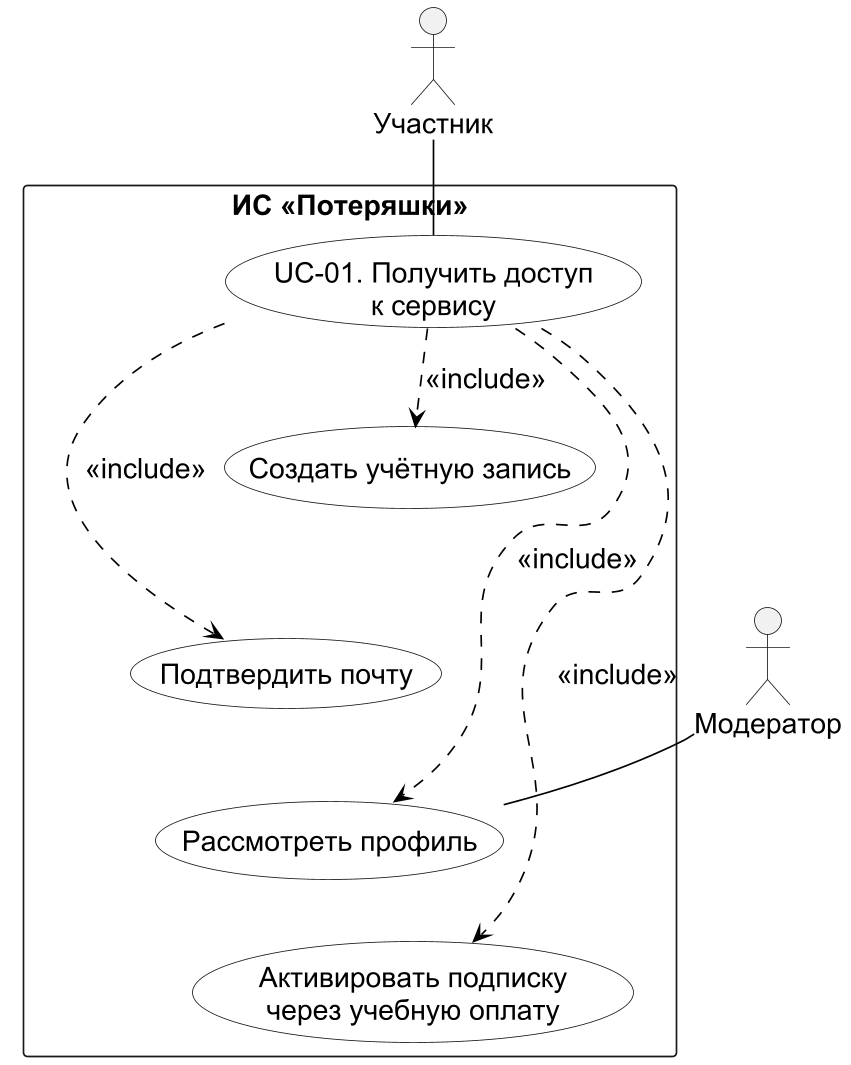
\includegraphics[width=\linewidth,height=0.82\textheight,keepaspectratio]{uml/revised/uc01_access.png}
\caption*{Рисунок 1 — Получение доступа к сервису}
\end{figure}
\FloatBarrier

\FloatBarrier
\Needspace{6\baselineskip}
\subsection{UC-02. Опубликовать находку}

Участник нашёл зонт в городском парке. Он создаёт карточку с местом и временем находки, прикладывает фотографию и оставляет надпись на внутренней стороне ручки закрытой приметой. Модератор проверяет объявление перед публикацией. После одобрения другие участники могут найти карточку в каталоге.

\begingroup
\setstretch{1}
\fontsize{12}{14}\selectfont
\setlength{\tablecontentwidth}{\dimexpr\linewidth-4\tabcolsep-3\arrayrulewidth\relax}
\begin{longtable}{|>{\RaggedRight\arraybackslash}p{0.25\tablecontentwidth}|>{\RaggedRight\arraybackslash}p{0.75\tablecontentwidth}|}
\hline
\textbf{Поле} & \textbf{Описание} \\ \hline
\endfirsthead
\textbf{Поле} & \textbf{Описание} \\ \hline
\endhead
\endfoot
\endlastfoot
ID & UC-02 \\ \hline
Цель & Опубликовать сведения о находке для поиска владельца. \\ \hline
Главный актёр & Участник — нашедший вещь. \\ \hline
Другой актёр & Модератор. \\ \hline
Предусловия & Автор вошёл в систему, профиль одобрен, подписка активна; категория и место доступны в справочниках. \\ \hline
Триггер & Нашедший выбирает создание объявления «Нашёл». \\ \hline
Постусловия & Проверенная карточка опубликована; закрытая примета сохраняется отдельно от публичного описания. \\ \hline
Требования & FR-04, FR-10; NFR-01, NFR-02, NFR-04. \\ \hline
\end{longtable}
\endgroup

Основной поток:

\begin{enumerate}
\item Нашедший открывает редактор и выбирает тип «Нашёл».
\item Он указывает название предмета, категорию, место, дату и время находки и описание.
\item Система проверяет обязательные поля и сохраняет черновик, связанный с автором.
\item Автор прикладывает фотографию зонта. Система проверяет JPEG/\allowbreak{}PNG и размер файла до 5 МБ и сохраняет изображение.
\item Автор записывает надпись на ручке как закрытую примету. Система не добавляет её в публичное описание.
\item Автор отправляет черновик на модерацию. Система меняет состояние объявления и помещает его в очередь.
\item Модератор просматривает описание и фотографии, проверяет соответствие правилам и отсутствие открытых персональных данных.
\item Модератор одобряет публикацию. Система фиксирует автора решения и время проверки.
\item Система открывает карточку для поиска в каталоге и сохраняет уведомление автору.
\item Нашедший проверяет опубликованную карточку и ожидает заявок владельцев.
\end{enumerate}

Альтернативные потоки:

\begin{itemize}
\item A1, шаги 2–3. Место, категория или время не указаны либо время находится в будущем: система показывает ошибку и сохраняет возможность исправить ввод.
\item A2, шаг 4. Формат или размер фотографии не подходит: файл отклоняется, черновик остаётся доступным; автор заменяет фотографию или публикует карточку без неё.
\item A3, шаг 8. Модератор отклоняет карточку: автор видит состояние объявления, исправляет описание или фотографию и повторяет отправку. Непроверенная версия в каталог не попадает.
\item A4, шаг 2. Вещь найдена в метро и передана сотруднику станции: автор указывает организацию хранения. В карточке показываются её контакты; личная заявка на получение у автора не создаётся.
\item A5, шаг 1. Автор сообщает о собственной потере: выбирает «Потерял», указывает предполагаемое место и допустимый интервал времени. Подготовка и модерация выполняются тем же порядком.
\end{itemize}

\FloatBarrier
\begin{figure}[htbp]
\centering
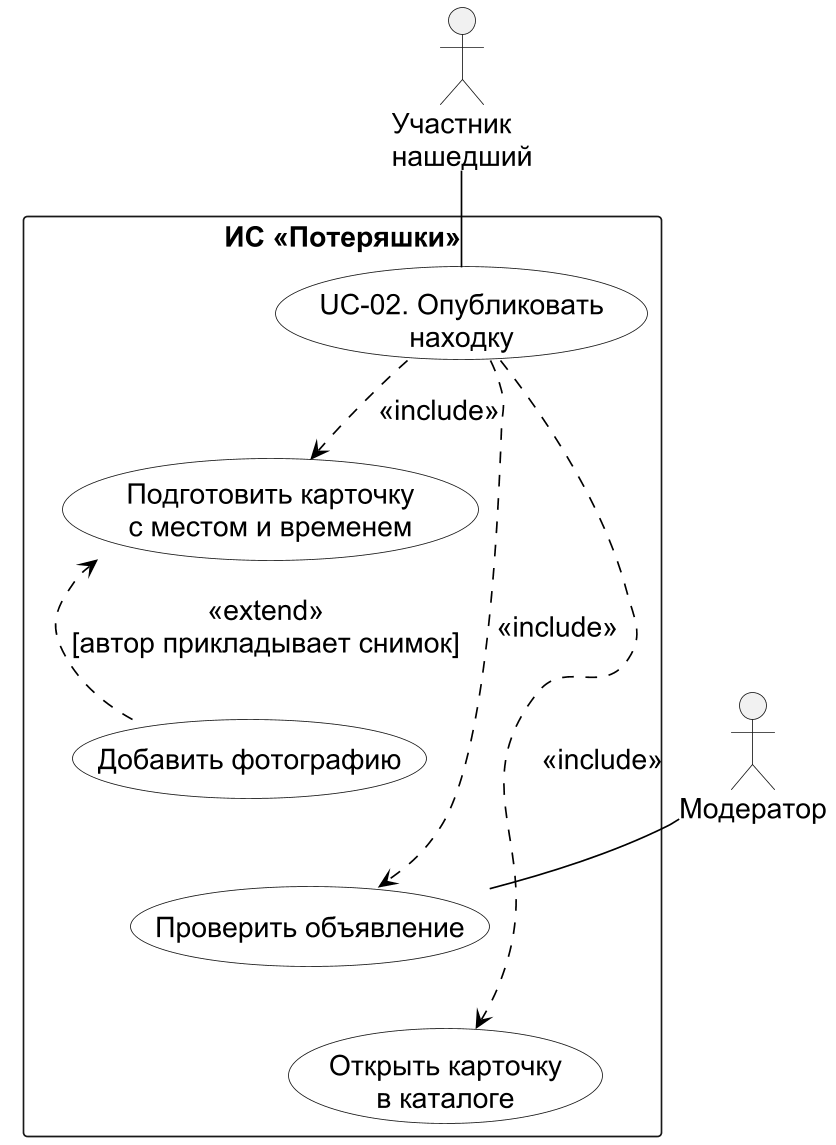
\includegraphics[width=\linewidth,height=0.82\textheight,keepaspectratio]{uml/revised/uc02_publish.png}
\caption*{Рисунок 2 — Публикация объявления о находке}
\end{figure}
\FloatBarrier

\FloatBarrier
\Needspace{6\baselineskip}
\subsection{UC-03. Вернуть вещь владельцу}

Другой участник потерял зонт и находит опубликованную карточку. Он сообщает нашедшему надпись на ручке, которую нельзя увидеть в каталоге. После проверки приметы стороны договариваются о встрече и отдельно подтверждают передачу. В этом процессе участвуют две разные учётные записи.

\begingroup
\setstretch{1}
\fontsize{12}{14}\selectfont
\setlength{\tablecontentwidth}{\dimexpr\linewidth-4\tabcolsep-3\arrayrulewidth\relax}
\begin{longtable}{|>{\RaggedRight\arraybackslash}p{0.25\tablecontentwidth}|>{\RaggedRight\arraybackslash}p{0.75\tablecontentwidth}|}
\hline
\textbf{Поле} & \textbf{Описание} \\ \hline
\endfirsthead
\textbf{Поле} & \textbf{Описание} \\ \hline
\endhead
\endfoot
\endlastfoot
ID & UC-03 \\ \hline
Цель & Передать найденную вещь подтверждённому владельцу и завершить поиск. \\ \hline
Главные актёры & Два участника — предполагаемый владелец и нашедший. \\ \hline
Предусловия & Оба участника вошли в систему; находка опубликована и хранится у автора; при создании заявки у владельца действует подписка; другого резерва и незавершённого аукциона нет. \\ \hline
Триггер & Предполагаемый владелец открывает карточку подходящей находки. \\ \hline
Постусловия & Выдача и получение подтверждены сторонами; дело завершено, находка отмечена возвращённой. \\ \hline
Требования & FR-05–07, FR-10; NFR-02, NFR-04, NFR-05. \\ \hline
\end{longtable}
\endgroup

Основной поток:

\begin{enumerate}
\item Владелец задаёт текст «зонт», категорию, место и примерный период потери.
\item Система показывает подходящие опубликованные карточки. Владелец открывает найденное объявление.
\item Владелец направляет заявку и описывает цвет, обстоятельства потери и закрытую надпись на ручке.
\item Система проверяет возможность заявки, сохраняет доказательства и создаёт закрытый диалог сторон.
\item Нашедший открывает заявку и сравнивает сведения с предметом и своей закрытой приметой.
\item Нашедший запрашивает уточнение в диалоге. Владелец отвечает, не публикуя личные контакты в каталоге.
\item Нашедший принимает заявку и согласовывает возврат.
\item Система резервирует находку за этим получателем и создаёт одно дело передачи.
\item Стороны договариваются о месте и времени встречи через диалог.
\item При встрече нашедший физически передаёт зонт и отмечает выдачу в своём кабинете.
\item Система сохраняет первое подтверждение; дело остаётся открытым до ответа другой стороны.
\item Владелец проверяет вещь и отдельно подтверждает получение.
\item Система завершает передачу, меняет состояние находки на «Возвращено» и сохраняет уведомления.
\end{enumerate}

Альтернативные потоки:

\begin{itemize}
\item A1, шаг 2. Подходящих карточек нет: владелец изменяет фильтры или публикует объявление о потере по UC-02. Процесс возврата пока не начинается.
\item A2, шаг 3. Находка хранится у метрополитена: система показывает официальный контакт, источник и инструкцию. Пользователь обращается в организацию вне приложения; личная заявка и резерв у автора не создаются.
\item A3, шаги 5–7. Приметы не совпадают: нашедший отклоняет заявку. Она сохраняется в истории, а вещь остаётся доступной другим претендентам.
\item A4, шаг 8. Другую заявку успели принять раньше: система отклоняет второй резерв. У одной находки остаётся один действующий получатель.
\item A5, шаг 9. Встреча отменена до подтверждений: владелец отменяет согласованную заявку, система освобождает находку. После первого подтверждения обычная отмена недоступна; участник обращается к модератору по UC-04.
\item A6, шаги 10–12. Подписка истекла после согласования: стороны могут прочитать существующий диалог и подтвердить уже начатую передачу без покупки новой подписки.
\item A7, шаг 12. Возник спор о выдаче или принадлежности: дело не считается завершённым, участник направляет жалобу по UC-04.
\end{itemize}

\FloatBarrier
\begin{figure}[htbp]
\centering
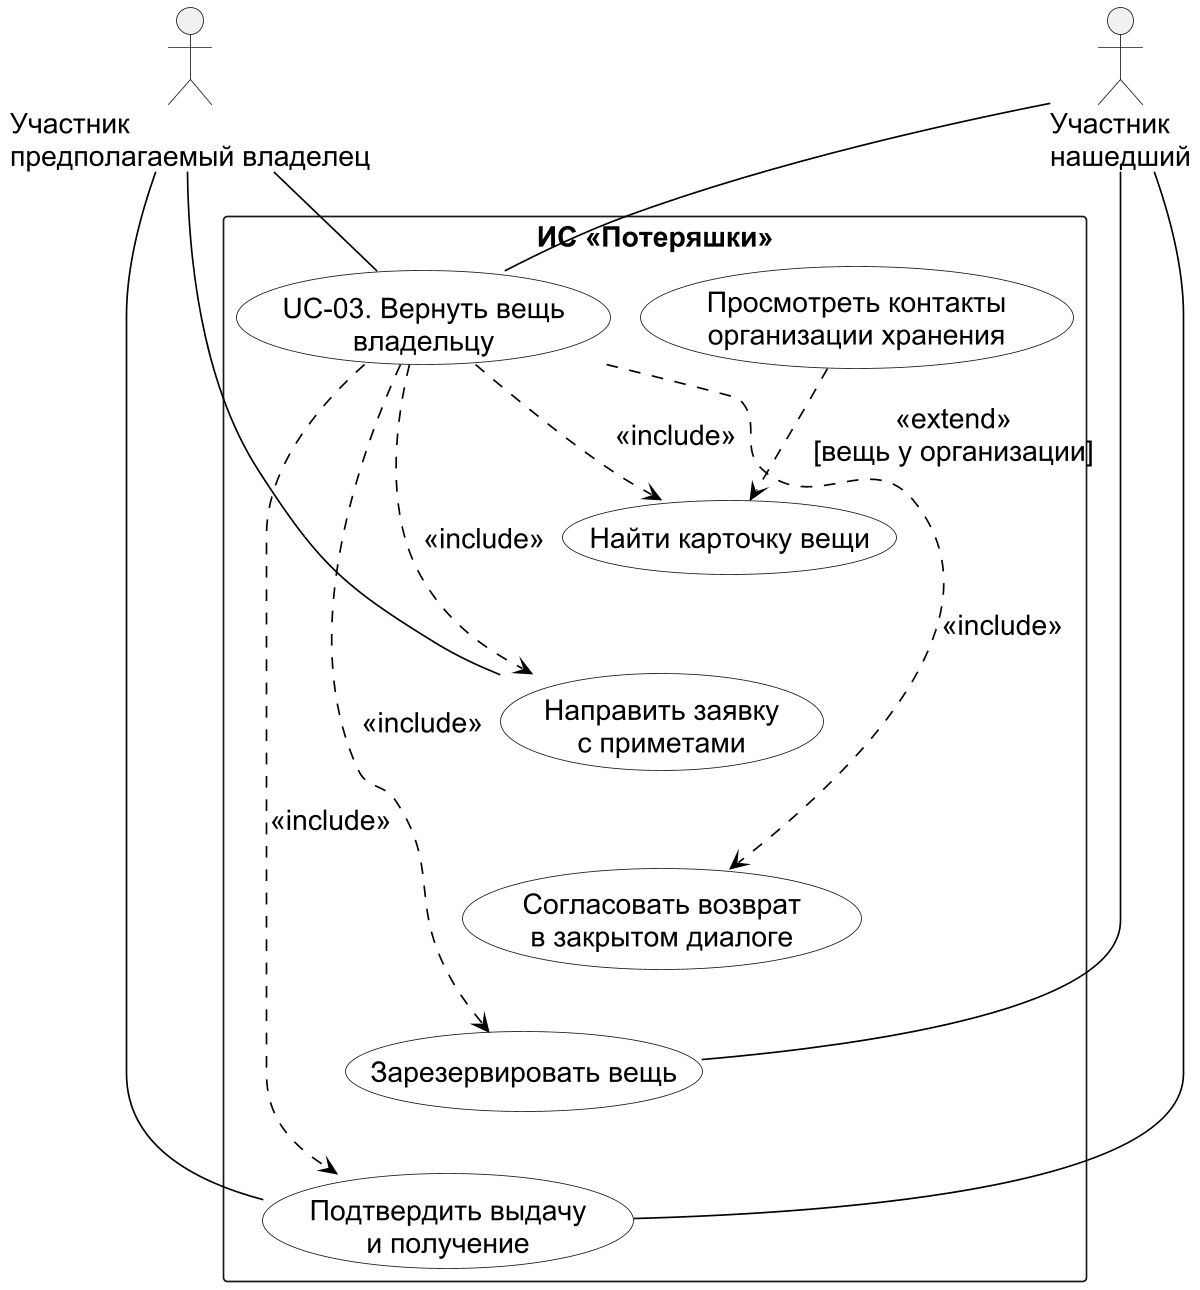
\includegraphics[width=\linewidth,height=0.82\textheight,keepaspectratio]{uml/revised/uc03_return.png}
\caption*{Рисунок 3 — Возврат вещи двумя участниками}
\end{figure}
\FloatBarrier

\FloatBarrier
\Needspace{6\baselineskip}
\subsection{UC-04. Разрешить спор о находке}

Нашедший отметил выдачу зонта, но предполагаемый владелец утверждает, что получил другую вещь, и не подтверждает получение. Обычная отмена уже недоступна. Участник направляет жалобу, независимый модератор изучает доказательства и переписку, получает пояснения сторон и принимает решение.

\begingroup
\setstretch{1}
\fontsize{12}{14}\selectfont
\setlength{\tablecontentwidth}{\dimexpr\linewidth-4\tabcolsep-3\arrayrulewidth\relax}
\begin{longtable}{|>{\RaggedRight\arraybackslash}p{0.25\tablecontentwidth}|>{\RaggedRight\arraybackslash}p{0.75\tablecontentwidth}|}
\hline
\textbf{Поле} & \textbf{Описание} \\ \hline
\endfirsthead
\textbf{Поле} & \textbf{Описание} \\ \hline
\endhead
\endfoot
\endlastfoot
ID & UC-04 \\ \hline
Цель & Разобрать конфликт по находке и сохранить решение по делу. \\ \hline
Главный актёр & Участник — заявитель жалобы. \\ \hline
Другие актёры & Другой участник дела; независимый модератор. \\ \hline
Предусловия & Существует объявление и связанное дело; заявитель вошёл в систему и участвует в деле; модератор не является автором спорного объявления или стороной жалобы. \\ \hline
Триггер & Участник подаёт жалобу с описанием противоречия. \\ \hline
Постусловия & Жалоба рассмотрена с указанием причины решения; при подтверждённой выдаче спорная передача завершена служебным решением. \\ \hline
Требования & FR-06, FR-08, FR-10; NFR-02, NFR-04. \\ \hline
\end{longtable}
\endgroup

Основной поток:

\begin{enumerate}
\item Заявитель открывает своё дело и направляет жалобу на объявление, описывая спор и обстоятельства встречи.
\item Система проверяет право обращения, сохраняет жалобу и показывает статус «Ожидает рассмотрения».
\item Независимый модератор открывает жалобу в служебной очереди.
\item Система предоставляет связанные заявки, признаки предмета и диалоги только на время рассмотрения открытой жалобы.
\item Модератор сопоставляет описание находки, доказательства владельца, сообщения и имеющееся подтверждение выдачи.
\item Модератор задаёт уточняющий вопрос в диалоге. Заявитель и нашедший отвечают со своих учётных записей.
\item После проверки выясняется, что передан тот же зонт, а заявитель неверно понял состояние предмета. Модератор формулирует причину решения о подтверждённой выдаче.
\item Модератор завершает спорную передачу служебным решением. Система сохраняет исполнителя и причину изменения состояния.
\item Модератор сохраняет решение по жалобе. Система закрывает её и уведомляет заявителя.
\item Заявитель читает результат в кабинете; другая сторона видит завершённое состояние передачи. Доступ сотрудника к закрытому диалогу по этой жалобе прекращается.
\end{enumerate}

Альтернативные потоки:

\begin{itemize}
\item A1, шаг 3. Модератор связан с жалобой: система не позволяет ему принять решение; дело рассматривает другой сотрудник с полномочиями модератора.
\item A2, шаги 5–7. Подтверждений фактической передачи недостаточно: модератор фиксирует решение по жалобе без завершения передачи. Находка не получает статус «Возвращено»; завершение возможно после подтверждений сторон или обоснованного служебного решения.
\item A3, шаг 7. Выявлено нарушение: модератор сохраняет решение об обоснованной жалобе и при необходимости блокирует нарушителя с указанием причины. Состояние передачи изменяется только отдельным допустимым действием.
\item A4, шаг 1. Подписка заявителя истекла: обращение по собственному ранее созданному делу остаётся доступным.
\item A5, шаг 9. Жалобу уже рассмотрел другой модератор: второе решение не записывается, сотрудник видит текущее состояние.
\end{itemize}

\FloatBarrier
\begin{figure}[htbp]
\centering
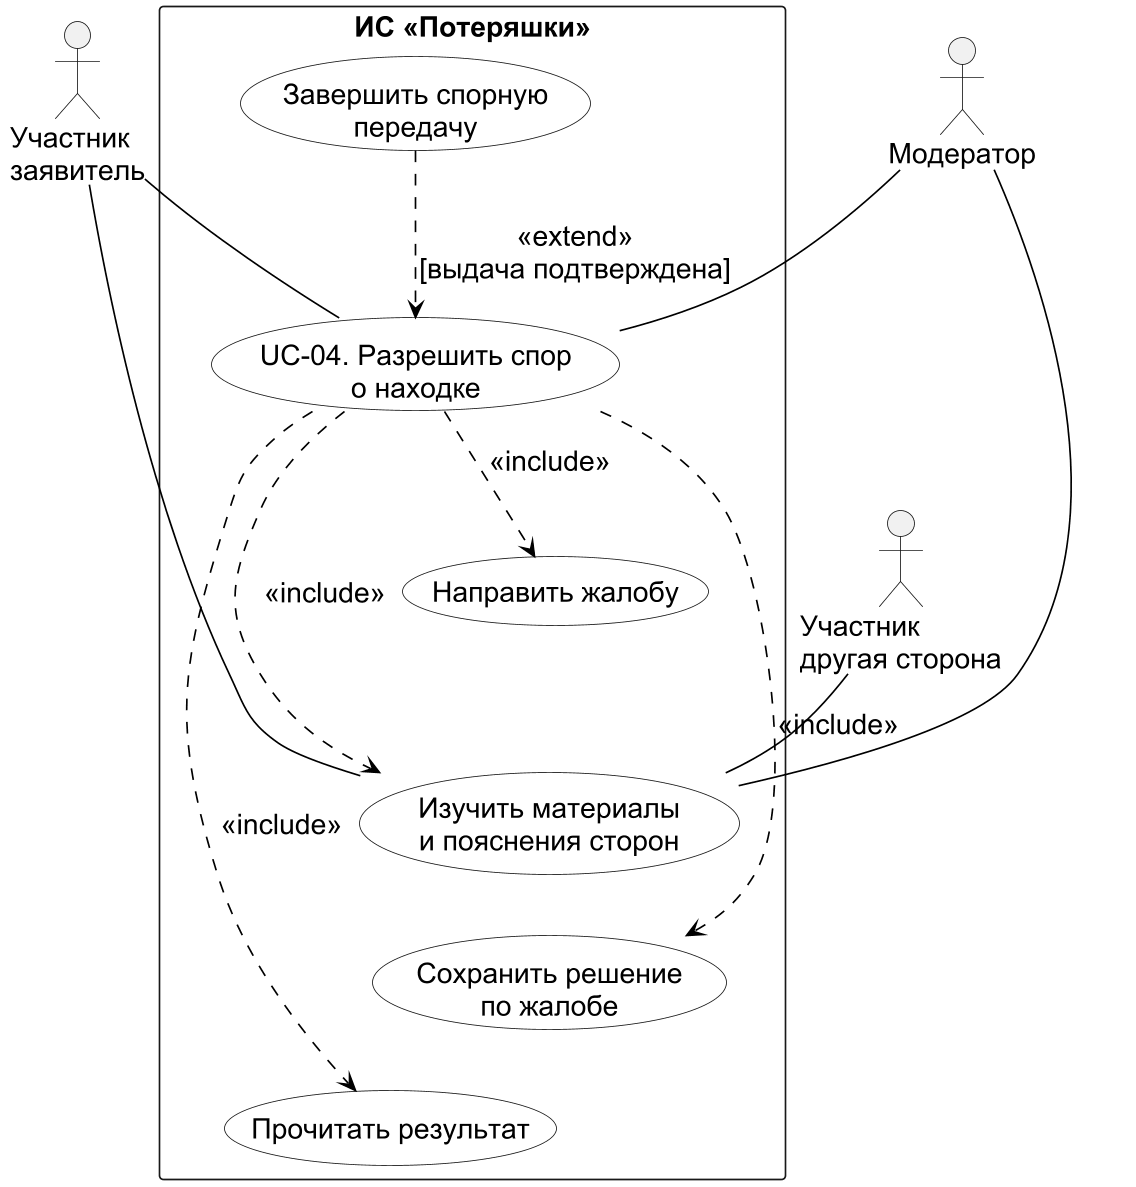
\includegraphics[width=\linewidth,height=0.82\textheight,keepaspectratio]{uml/revised/uc04_dispute.png}
\caption*{Рисунок 4 — Рассмотрение спора с участием сторон и модератора}
\end{figure}
\FloatBarrier

\FloatBarrier
\Needspace{6\baselineskip}
\subsection{UC-05. Продать вещь на аукционе}

Владелец другой находки не установлен. После выполнения предусмотренного порядка заявления и приобретения права распоряжения участник подаёт материалы на проверку. Модератор допускает продажу, два покупателя соревнуются ставками, а победитель согласовывает получение с продавцом. Давность объявления сама по себе не разрешает продажу.

\begingroup
\setstretch{1}
\fontsize{12}{14}\selectfont
\setlength{\tablecontentwidth}{\dimexpr\linewidth-4\tabcolsep-3\arrayrulewidth\relax}
\begin{longtable}{|>{\RaggedRight\arraybackslash}p{0.25\tablecontentwidth}|>{\RaggedRight\arraybackslash}p{0.75\tablecontentwidth}|}
\hline
\textbf{Поле} & \textbf{Описание} \\ \hline
\endfirsthead
\textbf{Поле} & \textbf{Описание} \\ \hline
\endhead
\endfoot
\endlastfoot
ID & UC-05 \\ \hline
Цель & Провести разрешённые торги и передать вещь победителю. \\ \hline
Главный актёр & Участник — продавец, имеющий основание распоряжения вещью. \\ \hline
Другие актёры & Участники — покупатели; независимый модератор. \\ \hline
Предусловия & Продавец проверен и имеет подписку; вещь хранится у него, относится к разрешённой категории и не зарезервирована для возврата; есть материалы основания распоряжения; открытого спора нет. \\ \hline
Триггер & Продавец подаёт заявку на допуск вещи к аукциону. \\ \hline
Постусловия & Победитель определён по принятой ставке; выдача и получение подтверждены продавцом и покупателем; история торгов сохранена. \\ \hline
Требования & FR-06, FR-09, FR-10; NFR-02, NFR-04, NFR-05. \\ \hline
\end{longtable}
\endgroup

Основной поток:

\begin{enumerate}
\item Продавец открывает свою находку и указывает основание распоряжения, дату официального заявления и подтверждающий документ.
\item Система проверяет обязательные сведения и сохраняет заявку на допуск.
\item Модератор изучает материалы и проверяет отсутствие запрета по категории, действующего возврата и открытого спора.
\item Модератор одобряет допуск с указанием причины. Система сохраняет решение.
\item Продавец создаёт лот, задаёт стартовую цену, шаг, начало и окончание торгов.
\item Система проверяет условия лота и сохраняет запланированный аукцион. Приём ставок возможен только в указанное время.
\item Первый покупатель открывает лот и направляет ставку.
\item Система проверяет доступ покупателя, время и сумму, сохраняет принятую ставку.
\item Другой покупатель предлагает большую сумму. Система последовательно проверяет и принимает подходящие предложения; продавец в своих торгах не участвует.
\item По окончании срока обработчик завершения определяет победителя по наибольшей принятой ставке.
\item Система сохраняет итог и создаёт одно дело передачи между продавцом и победителем с закрытым диалогом.
\item Продавец и победитель договариваются о встрече и расчёте вне приложения.
\item Продавец передаёт вещь и подтверждает выдачу; победитель подтверждает получение.
\item Система завершает передачу и сохраняет историю лота, ставок и подтверждений.
\end{enumerate}

Альтернативные потоки:

\begin{itemize}
\item A1, шаги 2–4. Основание не подтверждено, категория запрещена или есть спор: допуск отклоняется; лот не создаётся. Продавец видит причину и может исправить комплект материалов.
\item A2, шаг 8. Предложение поступило вне срока, не достигает допустимой суммы или отправлено продавцом: ставка отклоняется, текущая цена не меняется.
\item A3, шаг 9. Две ставки пришли одновременно: Postgre\allowbreak{}SQL обрабатывает их с блокировкой аукциона и повторно проверяет цену. Каждая принятая ставка соответствует актуальному шагу.
\item A4, шаг 10. Ставок нет: аукцион завершается без победителя и без дела передачи.
\item A5, шаги 6–9. На лот поступила претензия владельца: модератор рассматривает жалобу по UC-04 и при подтверждении основания отменяет незавершённые торги. Отменённый аукцион не принимает ставки; прежние предложения сохраняются в истории.
\item A6, шаги 8 или 10. Запрос ставки с тем же ключом либо завершение торгов повторены: система возвращает сохранённый результат, не создаёт дубликат ставки или второе дело передачи.
\item A7, шаг 13. После первого подтверждения стороны спорят о выдаче: передача остаётся открытой и разбирается по UC-04.
\end{itemize}

\FloatBarrier
\begin{figure}[htbp]
\centering
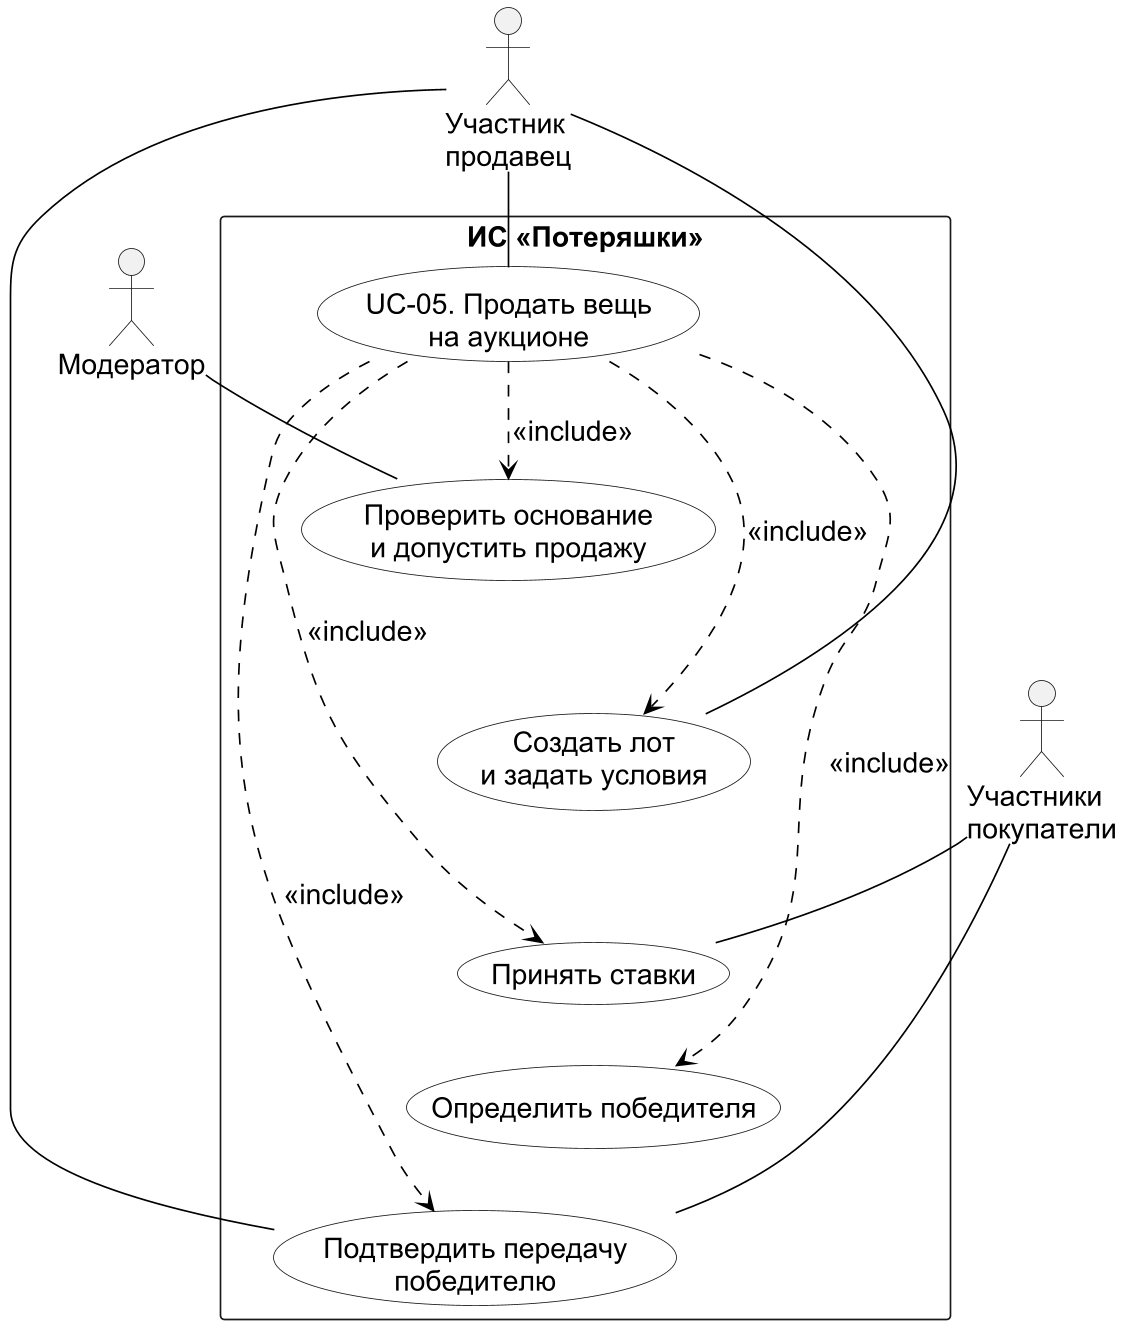
\includegraphics[width=\linewidth,height=0.82\textheight,keepaspectratio]{uml/revised/uc05_auction.png}
\caption*{Рисунок 5 — Аукцион с допуском, ставками и передачей победителю}
\end{figure}
\FloatBarrier

\clearpage
\section{Предлагаемая архитектура}

\FloatBarrier
\Needspace{6\baselineskip}
\subsection{Архитектурный подход и технологии}

Система проектируется как модульное монолитное приложение на Java 17. Одна JVM принимает HTTP-запросы, формирует страницы и выполняет прикладные операции. Postgre\allowbreak{}SQL и файловое хранилище отделены от процесса приложения. Модули предметной области разделяют ответственность, но используют общие правила доступа и транзакции.

\begingroup
\setstretch{1}
\fontsize{12}{14}\selectfont
\setlength{\tablecontentwidth}{\dimexpr\linewidth-6\tabcolsep-4\arrayrulewidth\relax}
\begin{longtable}{|>{\RaggedRight\arraybackslash}p{0.28\tablecontentwidth}|>{\RaggedRight\arraybackslash}p{0.32\tablecontentwidth}|>{\RaggedRight\arraybackslash}p{0.40\tablecontentwidth}|}
\caption{Архитектурный подход и технологии}\label{tab:22}\\
\hline
\textbf{Уровень} & \textbf{Технологии} & \textbf{Ответственность} \\ \hline
\endfirsthead
\multicolumn{3}{r}{\footnotesize Продолжение таблицы \thetable} \\
\hline
\textbf{Уровень} & \textbf{Технологии} & \textbf{Ответственность} \\ \hline
\endhead
\multicolumn{3}{r}{\footnotesize Продолжение на следующей странице} \\
\endfoot
\endlastfoot
Веб-сервер & Apache Tomcat, встроенный в Spring Boot & Приём HTTP-запросов и передача в цепочку фильтров и Spring MVC \\ \hline
Представление & Spring MVC, Thymeleaf, HTML, CSS & Страницы, формы, валидация параметров, отображение результатов и ошибок \\ \hline
Аутентификация & Spring Security, JWT, BCrypt & Проверка сеанса, защита форм CSRF, вход, выход и обновление токенов \\ \hline
Бизнес-логика & Java-сервисы, Access\allowbreak{}Policy, Spring Transactions & Правила процессов, права на объекты, координация действий и транзакционные границы \\ \hline
Хранение & Hibernate/\allowbreak{}JPA, Spring Data JPA, Jdbc\allowbreak{}Template & Проекции сущностей, параметризованные запросы, вызовы функций и процедур \\ \hline
База данных & Postgre\allowbreak{}SQL, PL/\allowbreak{}pg\allowbreak{}SQL & Связи, ограничения, триггеры, блокировки и критичные переходы состояний \\ \hline
Файловый адаптер & Закрытый локальный каталог, Java Image\allowbreak{}IO & Проверка фотографий, хранение вложений и выдача после проверки прав \\ \hline
Внешние адаптеры & Учебная оплата; почтовый интерфейс и SMTP & Подтверждение оплаты подписки, отправка писем и замена интеграций для демонстрации \\ \hline
Сборка и проверка & Gradle Wrapper, JUnit, Spring Test, Java-модуль tooling & Сборка JAR, интеграционные проверки, диаграммы, отчёты и установка на helios \\ \hline
\end{longtable}
\endgroup

Java, Spring Boot, Hibernate/\allowbreak{}JPA, Postgre\allowbreak{}SQL, Lombok и Gradle выбраны с учётом проекта My\allowbreak{}Film\allowbreak{}List [7]. Spring MVC и Thymeleaf позволяют включить контроллеры и представления в один JAR [8, 9]. Семейство Spring Boot 3.5 поддерживает выбранную версию Java [5]. Версии фиксируются в build.gradle. Изменения схемы представлены SQL-скриптами в Git; Hibernate проверяет соответствие сущностей существующей схеме и не создаёт таблицы при запуске.

Схема раскрывает устройство приложения «Потеряшки» внутри Spring Boot: встроенный Tomcat, фильтры Spring Security, MVC-контроллеры, HTML-шаблоны Thymeleaf, предметные сервисы, планировщик, репозитории и адаптеры. Узлы обозначают веб-сервер, компоненты — программные модули, артефакт — шаблоны, цилиндр — Postgre\allowbreak{}SQL, папка — закрытые вложения. Контроллеры вызывают сервисы и формируют модели страниц; сервисы используют JPA-репозитории и SQL-доступ через Jdbc\allowbreak{}Template. Postgre\allowbreak{}SQL и настраиваемый SMTP-сервер показаны вне приложения. Приложение размещается на helios; браузер подключается по HTTP через SSH-туннель.

\begin{figure}[htbp]
\centering
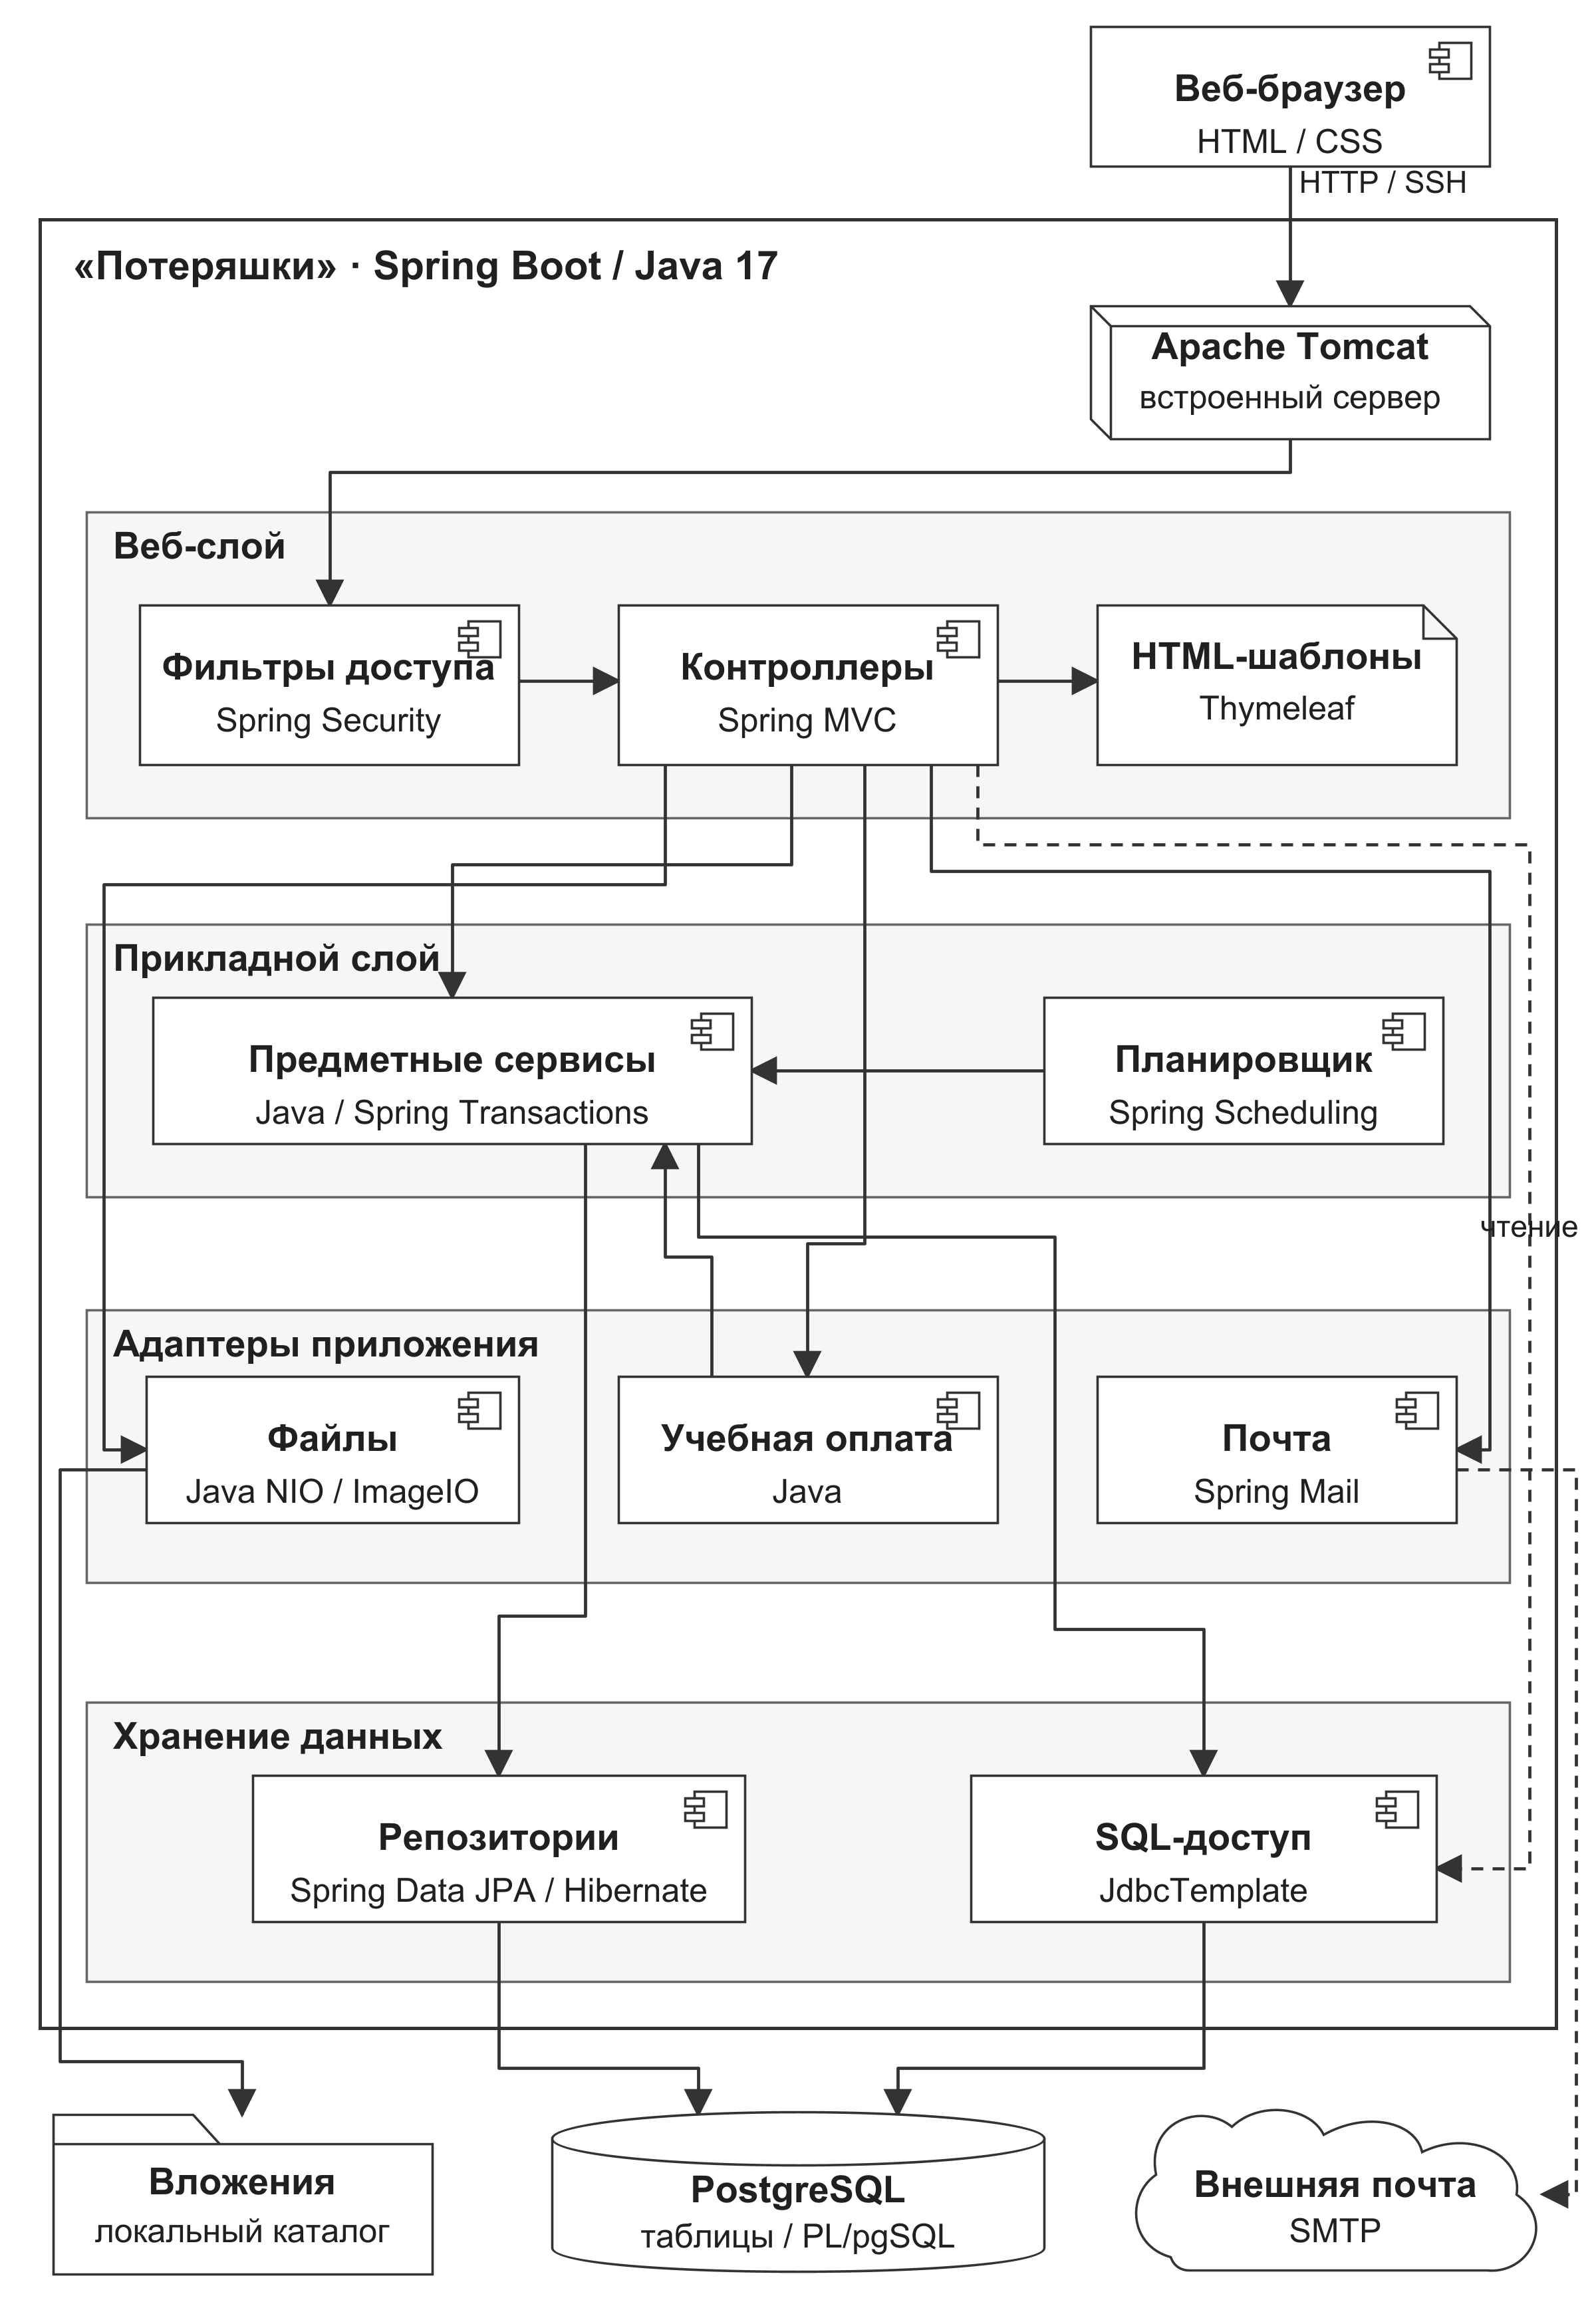
\includegraphics[width=\linewidth,height=0.82\textheight,keepaspectratio]{uml/revised/system_architecture.png}
\caption*{Рисунок 6 — Общая архитектура информационной системы}
\end{figure}

\FloatBarrier
\Needspace{6\baselineskip}
\subsection{Компоненты и распределение ответственности}

\begingroup
\setstretch{1}
\fontsize{12}{14}\selectfont
\setlength{\tablecontentwidth}{\dimexpr\linewidth-6\tabcolsep-4\arrayrulewidth\relax}
\begin{longtable}{|>{\RaggedRight\arraybackslash}p{0.28\tablecontentwidth}|>{\RaggedRight\arraybackslash}p{0.32\tablecontentwidth}|>{\RaggedRight\arraybackslash}p{0.40\tablecontentwidth}|}
\caption{Компоненты и распределение ответственности}\label{tab:23}\\
\hline
\textbf{Компонент} & \textbf{Вход и результат} & \textbf{Основные зависимости} \\ \hline
\endfirsthead
\multicolumn{3}{r}{\footnotesize Продолжение таблицы \thetable} \\
\hline
\textbf{Компонент} & \textbf{Вход и результат} & \textbf{Основные зависимости} \\ \hline
\endhead
\multicolumn{3}{r}{\footnotesize Продолжение на следующей странице} \\
\endfoot
\endlastfoot
Web\allowbreak{}Sessions, Web\allowbreak{}Identity, Spring Security & Проверенный сеанс и идентификатор действующего пользователя & Хеши паролей, версии токенов и отозванные сеансы в Postgre\allowbreak{}SQL \\ \hline
MVC-контроллеры & Параметры форм; модель страницы либо перенаправление & Сервисы предметной области и Thymeleaf \\ \hline
Web\allowbreak{}Queries & Проекции для каталога, кабинета и очередей & Sql\allowbreak{}Store и проверки доступа; публичные проекции исключают секреты \\ \hline
Account\allowbreak{}Service, Subscription\allowbreak{}Service & Подтверждённый профиль, заказ и оплаченный период; UC-01 & Access\allowbreak{}Policy, почтовый и платёжный адаптеры, Database\allowbreak{}Functions \\ \hline
Listing\allowbreak{}Service & Черновик, публикация, фильтры и карточка; UC-02 и начало UC-03 & Access\allowbreak{}Policy, Sql\allowbreak{}Store, поиск PL/\allowbreak{}pg\allowbreak{}SQL и файловый адаптер \\ \hline
Return\allowbreak{}Service & Заявка, диалог, резерв и подтверждения; UC-03 & Проверка участников и функции резервирования и передачи \\ \hline
Administration\allowbreak{}Service & Жалоба, служебное решение, роли, тарифы, организации; UC-04, служебное управление & Access\allowbreak{}Policy, Sql\allowbreak{}Store и неизменяемый аудит \\ \hline
Auction\allowbreak{}Service & Допуск, лот, ставка и итог; UC-05 & Функции торгов, запись находки и проверка права продавца \\ \hline
Outbox\allowbreak{}Service, Web\allowbreak{}Jobs & Доставка уведомлений и закрытие истёкших торгов & Очередь событий и процедура Postgre\allowbreak{}SQL; повторная обработка безопасна \\ \hline
Sql\allowbreak{}Store, репозитории JPA, Database\allowbreak{}Functions & Параметризованные операции хранения & JDBC-пул и схема Postgre\allowbreak{}SQL \\ \hline
Private\allowbreak{}Files, Media\allowbreak{}Pages & Проверенный файл и разрешённая выдача & Закрытый каталог и проверка владельца либо служебных полномочий \\ \hline
\end{longtable}
\endgroup

Роль инициатора определяется по проверенному сеансу. Контроллер не принимает идентификатор действующего пользователя из скрытого поля формы. Access\allowbreak{}Policy проверяет роль, состояние профиля, подписку и принадлежность объекта в серверном коде; скрытие кнопки не заменяет эту проверку. Для модератора отдельно проверяется отсутствие заинтересованности в рассматриваемом деле.

Модели Thymeleaf содержат только сведения, нужные странице. Пароли, хеши токенов и чужие закрытые признаки в них не включаются. Служебная очередь и публичный каталог используют разные проекции. Шаблоны находятся в src/\allowbreak{}main/\allowbreak{}resources/\allowbreak{}templates, стили — в src/\allowbreak{}main/\allowbreak{}resources/\allowbreak{}static и включаются в JAR.

\FloatBarrier
\Needspace{6\baselineskip}
\subsection{Обработка запроса на примере возврата}

\begin{enumerate}
\item Владелец открывает опубликованную находку. Spring Security проверяет токен и текущий сеанс; контроллер получает идентификатор пользователя через Web\allowbreak{}Identity.
\item Контроллер передаёт заявку и доказательства в Return\allowbreak{}Service. Access\allowbreak{}Policy проверяет доступ, сервис создаёт заявку и диалог в одной транзакции и сохраняет событие уведомления.
\item Нашедший открывает дело из своего кабинета. Проверка принадлежности даёт доступ только участникам заявки; во время открытого спора допускается независимый модератор.
\item После уточнений нашедший подтверждает согласование. Database\allowbreak{}Functions вызывает lf\_\allowbreak{}reserve\_\allowbreak{}found; функция блокирует находку, проверяет отсутствие другого резерва и создаёт передачу.
\item Первое подтверждение вызывает lf\_\allowbreak{}confirm\_\allowbreak{}transfer и сохраняет одну отметку. Второе завершает передачу, заявку и состояние находки той же функцией.
\item Контроллер возвращает обновлённую страницу. Outbox\allowbreak{}Service доставляет уведомления после фиксации транзакции. Ошибка внешнего адаптера не отменяет уже сохранённый результат возврата.
\end{enumerate}

В UC-03 нашедший и владелец используют разные учётные записи. Их обращения поступают через контроллеры; проверка прав, резервирование и подтверждение передачи выполняются на сервере.

\FloatBarrier
\Needspace{6\baselineskip}
\subsection{Хранение и транзакционные границы}

В Postgre\allowbreak{}SQL размещаются учётные записи, назначения ролей, токены, проверки профилей, тарифы и заказы, подписки, объявления, справочники, заявки, сообщения, передачи, жалобы, допуски, аукционы, ставки, уведомления, очередь событий и аудит. Таблица назначений ролей образует связь M:N между пользователями и ролями. Конкретные таблицы, атрибуты и ограничения разрабатываются на втором этапе.

Критичные операции реализуются функциями PL/\allowbreak{}pg\allowbreak{}SQL: активация подписки, поиск, резервирование, подтверждение передачи, приём ставки и завершение торгов. Третий этап должен вызывать эти функции из Java, сохраняя правила и блокировки в базе. Прикладной слой проверяет пользователя, подготавливает параметры и обрабатывает результат.

\begingroup
\setstretch{1}
\fontsize{12}{14}\selectfont
\setlength{\tablecontentwidth}{\dimexpr\linewidth-6\tabcolsep-4\arrayrulewidth\relax}
\begin{longtable}{|>{\RaggedRight\arraybackslash}p{0.28\tablecontentwidth}|>{\RaggedRight\arraybackslash}p{0.32\tablecontentwidth}|>{\RaggedRight\arraybackslash}p{0.40\tablecontentwidth}|}
\caption{Хранение и транзакционные границы}\label{tab:24}\\
\hline
\textbf{Операция} & \textbf{Транзакционная граница} & \textbf{Защита от конфликта} \\ \hline
\endfirsthead
\multicolumn{3}{r}{\footnotesize Продолжение таблицы \thetable} \\
\hline
\textbf{Операция} & \textbf{Транзакционная граница} & \textbf{Защита от конфликта} \\ \hline
\endhead
\multicolumn{3}{r}{\footnotesize Продолжение на следующей странице} \\
\endfoot
\endlastfoot
Оплата подписки & Событие оплаты и один оплаченный период & Ключ события, блокировки пользователя и заказа, отсутствие повторного продления \\ \hline
Согласование возврата & Принятая заявка, резерв, передача и событие & Блокировка находки, один действующий резерв и отсутствие незавершённых торгов \\ \hline
Подтверждение передачи & Отметка стороны либо завершение всего дела & Блокировка состояния дела и проверка участников \\ \hline
Приём ставки & Проверенная ставка и событие уведомления & Единый порядок блокировок: находка, затем аукцион; повторная проверка времени и цены \\ \hline
Завершение торгов & Победитель, итог и единственное дело передачи & Те же блокировки, запрет ставки после окончания, идемпотентный повтор \\ \hline
Служебное решение & Изменение состояния и аудит & Проверка независимости, полномочий и допустимого перехода \\ \hline
\end{longtable}
\endgroup

Для денежных значений применяется NUMERIC(12,2), для моментов времени — timestamptz. Ввод и отображение используют Europe/\allowbreak{}Moscow. Поиск выполняется средствами Postgre\allowbreak{}SQL: индексы по месту, категории, типу и состоянию, полнотекстовый индекс по русскому описанию. Состав и полезность индексов обосновываются на втором этапе по прецедентам.

Outbox хранит событие вместе с бизнес-изменением в одной транзакции. Отдельный обработчик выбирает недоставленные записи, создаёт внутренние уведомления и отмечает доставку. Аудит фиксирует исполнителя, объект, действие, время и результат; пользовательские операции не редактируют журнал.

\FloatBarrier
\Needspace{6\baselineskip}
\subsection{Файлы и внешние интеграции}

Фотографии и подтверждающие материалы хранятся отдельно от статических ресурсов. В базе находятся ключ файла, тип, размер и связь с объявлением либо допуском. Фотография декодируется, проверяется и пересохраняется без исходных метаданных. Выдача файла идёт через контроллер с проверкой прав. Документ допуска доступен продавцу и модератору; публичный каталог его не раскрывает.

Для учебной установки выбран закрытый локальный каталог STORAGE\_\allowbreak{}ROOT. Min\allowbreak{}IO может заменить файловый адаптер при дальнейшем развитии; такой вариант требует настройки закрытого бакета и совместного резервного копирования базы и объектов. Он не является зависимостью первоначального запуска на helios.

Платёжный адаптер подтверждает оплату подписки, а не расчёт между продавцом и покупателем лота. Учебный режим не списывает средства и проверяет повторные результаты. При подключении внешнего провайдера результат должен проверяться адаптером до вызова функции активации подписки.

Почтовый интерфейс используется для подтверждения адреса и восстановления доступа. В учебном режиме письма доступны получателю в его кабинете; для внешней доставки предусмотрены параметры SMTP и STARTTLS. Внутренние уведомления сохраняются в Postgre\allowbreak{}SQL независимо от почтовой доставки.

Справочная интеграция метро читает данные из справочника организаций. Администратор обновляет запись по официальному источнику согласно FR-07. Запрос к каталогу или инструкции не зависит от доступности сайта метрополитена; прямой обмен реестрами не предусматривается.

\clearpage
\section*{Вывод}
\phantomsection
\addcontentsline{toc}{section}{Вывод}

Определены предметная область, три роли доступа и пять подробных прецедентов с законченным результатом. Описаны взаимодействия участников, модератора и администратора, основные и альтернативные потоки. Сформулированы десять функциональных и шесть нефункциональных требований, соответствующих учебной реализации. Архитектура разделяет представление, проверку сеанса, предметные сервисы, хранение и адаптеры. Java-приложение на Spring MVC и Thymeleaf размещается на helios, данные — в Postgre\allowbreak{}SQL, вложения — в закрытом каталоге. Min\allowbreak{}IO рассматривается как расширение файлового адаптера.

Второй этап включает ER-модель, даталогическую модель, схему Postgre\allowbreak{}SQL, ограничения и триггеры, тестовые данные, функции PL/\allowbreak{}pg\allowbreak{}SQL и индексы. Реализация интерфейса и серверного приложения относится к последующим этапам.

\clearpage
\section*{Список использованных источников}
\phantomsection
\addcontentsline{toc}{section}{Список использованных источников}

Дата проверки источников: 03.10.2026. Контакты и условия организации подлежат повторной проверке перед эксплуатацией. Все проектные требования и численные цели сформулированы для данной курсовой; они не являются требованиями метрополитена.

\begin{enumerate}[label={[\arabic*]},leftmargin=10mm]
\RaggedRight
\item Петербургский метрополитен. Справочная о забытых вещах. Официальный источник порядка хранения и получения: \url{https://metro.spb.ru/zabitieveshy.html?v=1}
\item Петербургский метрополитен. Контакты. Проверка телефона информационно-справочного центра: \url{https://metro.spb.ru/contacts.html}
\item Гражданский кодекс Российской Федерации, часть первая, статья 227 «Находка». Текст нормы в СПС «КонсультантПлюс»: \url{https://www.consultant.ru/document/cons_doc_LAW_5142/b3526f37d7093a56bf084817caeee175f032a3d7/}
\item Гражданский кодекс Российской Федерации, часть первая, статья 228 «Приобретение права собственности на находку». Текст нормы в СПС «КонсультантПлюс»: \url{https://www.consultant.ru/document/cons_doc_LAW_5142/104dea7aa78d4c2e927d3baed4e96d5ace10e692/}
\item Spring. Spring Boot 3.5 — System Requirements. Официальная документация: \url{https://docs.spring.io/spring-boot/3.5/system-requirements.html}
\item Кафедра ВТ, Университет ИТМО. Программирование. Публичные задания с демонстрацией Java-программ на helios: \url{https://se.ifmo.ru/courses/programming}
\item My\allowbreak{}Film\allowbreak{}List. Backend, build.gradle, версия \nolinkurl{74d1928973cae329d6ca651bac2ffde445a43de0}: \url{https://github.com/maxbarsukov/MyFilmList/blob/74d1928973cae329d6ca651bac2ffde445a43de0/build.gradle}
\item Spring Framework. Thymeleaf: \url{https://docs.spring.io/spring-framework/reference/web/webmvc-view/mvc-thymeleaf.html}
\item Thymeleaf. Интеграция со Spring: \url{https://www.thymeleaf.org/doc/tutorials/3.1/thymeleafspring.html}
\end{enumerate}

\clearpage
\section*{Приложение А. Термины}
\phantomsection
\addcontentsline{toc}{section}{Приложение А. Термины}

\begingroup
\setstretch{1}
\fontsize{12}{14}\selectfont
\setlength{\tablecontentwidth}{\dimexpr\linewidth-4\tabcolsep-3\arrayrulewidth\relax}
\begin{longtable}{|>{\RaggedRight\arraybackslash}p{0.27\tablecontentwidth}|>{\RaggedRight\arraybackslash}p{0.73\tablecontentwidth}|}
\caption{Приложение А. Термины}\label{tab:25}\\
\hline
\textbf{Термин} & \textbf{Определение} \\ \hline
\endfirsthead
\multicolumn{2}{r}{\footnotesize Продолжение таблицы \thetable} \\
\hline
\textbf{Термин} & \textbf{Определение} \\ \hline
\endhead
\multicolumn{2}{r}{\footnotesize Продолжение на следующей странице} \\
\endfoot
\endlastfoot
Верификация профиля & Подтверждение почты и решение модератора о допуске аккаунта; не паспортная идентификация \\ \hline
Подписка & Оплаченный период доступа к пользовательским функциям \\ \hline
Контрольный признак & Непубличная характеристика вещи для проверки претендента \\ \hline
Резервирование & Согласование выдачи одной находки одному претенденту \\ \hline
Справочная интеграция & Подбор проверенных контактов и инструкций организации без обмена её внутренними данными \\ \hline
Допуск аукциона & Решение модератора по материалам основания распоряжения вещью \\ \hline
Идемпотентность & Повтор запроса или события не создаёт повторный результат операции \\ \hline
Outbox & Таблица событий, записываемых вместе с бизнес-операцией для последующей надёжной доставки \\ \hline
\end{longtable}
\endgroup

\clearpage
\section*{Приложение Б. Соответствие заданию и проверка требований}
\phantomsection
\addcontentsline{toc}{section}{Приложение Б. Соответствие заданию и проверка требований}

\begingroup
\setstretch{1}
\fontsize{12}{14}\selectfont
\setlength{\tablecontentwidth}{\dimexpr\linewidth-6\tabcolsep-4\arrayrulewidth\relax}
\begin{longtable}{|>{\RaggedRight\arraybackslash}p{0.30\tablecontentwidth}|>{\RaggedRight\arraybackslash}p{0.18\tablecontentwidth}|>{\RaggedRight\arraybackslash}p{0.52\tablecontentwidth}|}
\hline
\textbf{Пункт задания} & \textbf{Раздел отчёта} & \textbf{Результат} \\ \hline
\endfirsthead
\textbf{Пункт задания} & \textbf{Раздел отчёта} & \textbf{Результат} \\ \hline
\endhead
\endfoot
\endlastfoot
1. Выбор предметной области & 1–2 & Поиск и возврат потерянных вещей в Санкт-Петербурге \\ \hline
2. Подробное описание & 2 & Участники, процессы, данные и правила работы с находками \\ \hline
3. Назначение системы & 3 & Цель и задачи автоматизации \\ \hline
4. Требования & 4 & Десять функциональных и шесть нефункциональных требований \\ \hline
5. Прецеденты & 5 & Пять подробных процессов и отдельная диаграмма каждого \\ \hline
6. Архитектура & 6 & Общая схема приложения, Postgre\allowbreak{}SQL, файлов и доступа через helios \\ \hline
7. Отчёт & Весь документ & Анализ предметной области и проектирование системы \\ \hline
\end{longtable}
\endgroup

\begingroup
\setstretch{1}
\fontsize{12}{14}\selectfont
\setlength{\tablecontentwidth}{\dimexpr\linewidth-4\tabcolsep-3\arrayrulewidth\relax}
\begin{longtable}{|>{\RaggedRight\arraybackslash}p{0.25\tablecontentwidth}|>{\RaggedRight\arraybackslash}p{0.75\tablecontentwidth}|}
\hline
\textbf{Прецедент} & \textbf{Связанные функциональные требования} \\ \hline
\endfirsthead
\textbf{Прецедент} & \textbf{Связанные функциональные требования} \\ \hline
\endhead
\endfoot
\endlastfoot
UC-01. Получить доступ к сервису & FR-01, FR-02, FR-03, FR-10 \\ \hline
UC-02. Опубликовать находку & FR-04, FR-10 \\ \hline
UC-03. Вернуть вещь владельцу & FR-05, FR-06, FR-07, FR-10 \\ \hline
UC-04. Разрешить спор о находке & FR-06, FR-08, FR-10 \\ \hline
UC-05. Продать вещь на аукционе & FR-06, FR-09, FR-10 \\ \hline
\end{longtable}
\endgroup

Функциональные требования проверяются прохождением этих пяти процессов с разными учётными записями. В UC-03 отдельно проверяется обращение к справочнику метро вместо личной заявки на вещь, переданную организации. Демонстрационная оплата не требует подключения платёжного провайдера.

Для NFR-01 проверяются формы на компьютере и телефоне; для NFR-02 — отказ в доступе к чужим материалам; для NFR-03 — отсутствие исходных паролей в базе, ответах и журнале. NFR-04 проверяется параллельным резервированием и откатом неуспешной операции, NFR-05 — повтором одного запроса или события. NFR-06 проверяется запуском JAR с указанным ограничением heap и доступом через SSH-туннель к Postgre\allowbreak{}SQL и файлам курсовой.


\clearpage
\section*{Задание второго этапа}
\phantomsection
\addcontentsline{toc}{section}{Задание второго этапа}

Второй этап курсовой работы включает:

\begin{enumerate}
\item Построение ER-модели не менее чем с 10 сущностями и связью «многие ко многим».
\item Построение даталогической модели на основе ER-модели.
\item Реализацию модели в Postgre\allowbreak{}SQL.
\item Обеспечение целостности средствами DDL и триггеров.
\item Скрипты создания, удаления и заполнения тестовыми данными.
\item Функции и процедуры PL/\allowbreak{}pg\allowbreak{}SQL для критически важных запросов.
\item Индексы по прецедентам первого этапа и обоснование их полезности.
\item Подготовку отчёта.
\end{enumerate}

\clearpage
\section{ER-модель базы данных}

\FloatBarrier
\Needspace{6\baselineskip}
\subsection{Сущности и связи}

Модель построена по процессам и прецедентам первого этапа и содержит 27 сущностей: пользователи, роли, назначения ролей, проверки профилей, одноразовые токены, токены обновления, тарифы, заказы оплаты, платёжные события, периоды подписки, организации, места, категории, объявления, изображения, контрольные признаки, заявки на передачу, диалоги, сообщения, передачи, жалобы, допуски к продаже, аукционы, ставки, уведомления, события доставки и записи аудита.

Пользователь может иметь несколько ролей, а одна роль назначается нескольким пользователям. Отношение «многие ко многим» реализовано ассоциативной сущностью «Назначение роли»: lf\_\allowbreak{}user\_\allowbreak{}roles(user\_\allowbreak{}id, role\_\allowbreak{}code). Составной первичный ключ исключает повторное назначение одной роли пользователю.

Объявление принадлежит одному автору, одной категории и одному месту. Место может быть связано с организацией, предоставляющей справочную информацию. Организация-хранитель находки задаётся отдельно: событие могло произойти в одном месте, а вещь передана другой организации. Поле custodian\_\allowbreak{}org\_\allowbreak{}id не означает партнёрство организации с приложением.

Заявка связывает находку с претендентом. У находки может быть несколько заявок, но один действующий резерв. Диалог и передача относятся к конкретной заявке; участники определяются через автора объявления и заявителя. Необязательный auction\_\allowbreak{}id с внешним ключом и UNIQUE связывает дело передачи с завершённым аукционом: одному аукциону соответствует не более одного такого дела. Допуск к продаже относится к находке и продавцу; каждый аукцион использует конкретный допуск. Это исключает подстановку разрешения для другой вещи. Всего модель содержит 42 внешних ключа.

Заказ оплаты фиксирует стоимость и длительность тарифа на момент создания. Изменение справочника тарифов не меняет уже созданный заказ. Внешние события оплаты отделены от периодов подписки, поскольку платёжный сервис может повторить событие. Одному оплаченному заказу соответствует не более одного периода.

Уведомление адресовано пользователю. Событие доставки содержит тип агрегата, его идентификатор и JSON-параметры; эта техническая очередь не имеет универсального внешнего ключа на разные таблицы. Аудит хранит таблицу и идентификатор изменённой сущности. Его actor\_\allowbreak{}id может быть NULL для фоновой операции.

\FloatBarrier
\Needspace{6\baselineskip}
\subsection{Диаграммы}

Модель разделена на шесть листов для чтения в формате A4. Листы показывают основные связи и их мощности; повтор сущности на разных листах не означает дополнительную таблицу. Полный перечень внешних ключей и атрибутов приведён в даталогической модели и словаре отношений. Обозначения: 1 — ровно один, 0..1 — необязательный экземпляр, 0..N — множество.

\FloatBarrier
\begin{figure}[htbp]
\centering
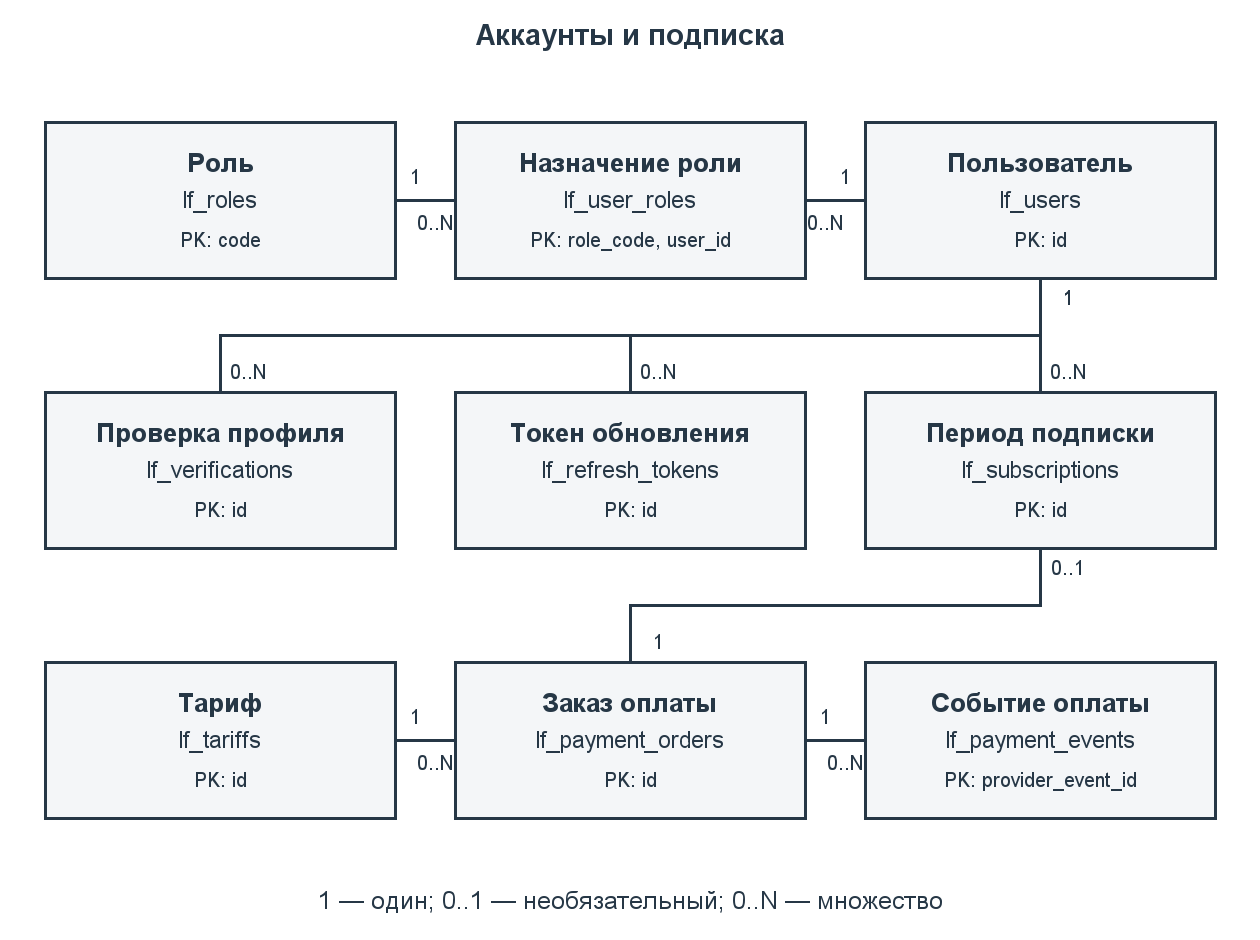
\includegraphics[width=\linewidth,height=0.82\textheight,keepaspectratio]{model/01_accounts.png}
\caption*{Рисунок 7 — ER-модель: аккаунты и подписка}
\end{figure}
\FloatBarrier

\FloatBarrier
\begin{figure}[htbp]
\centering
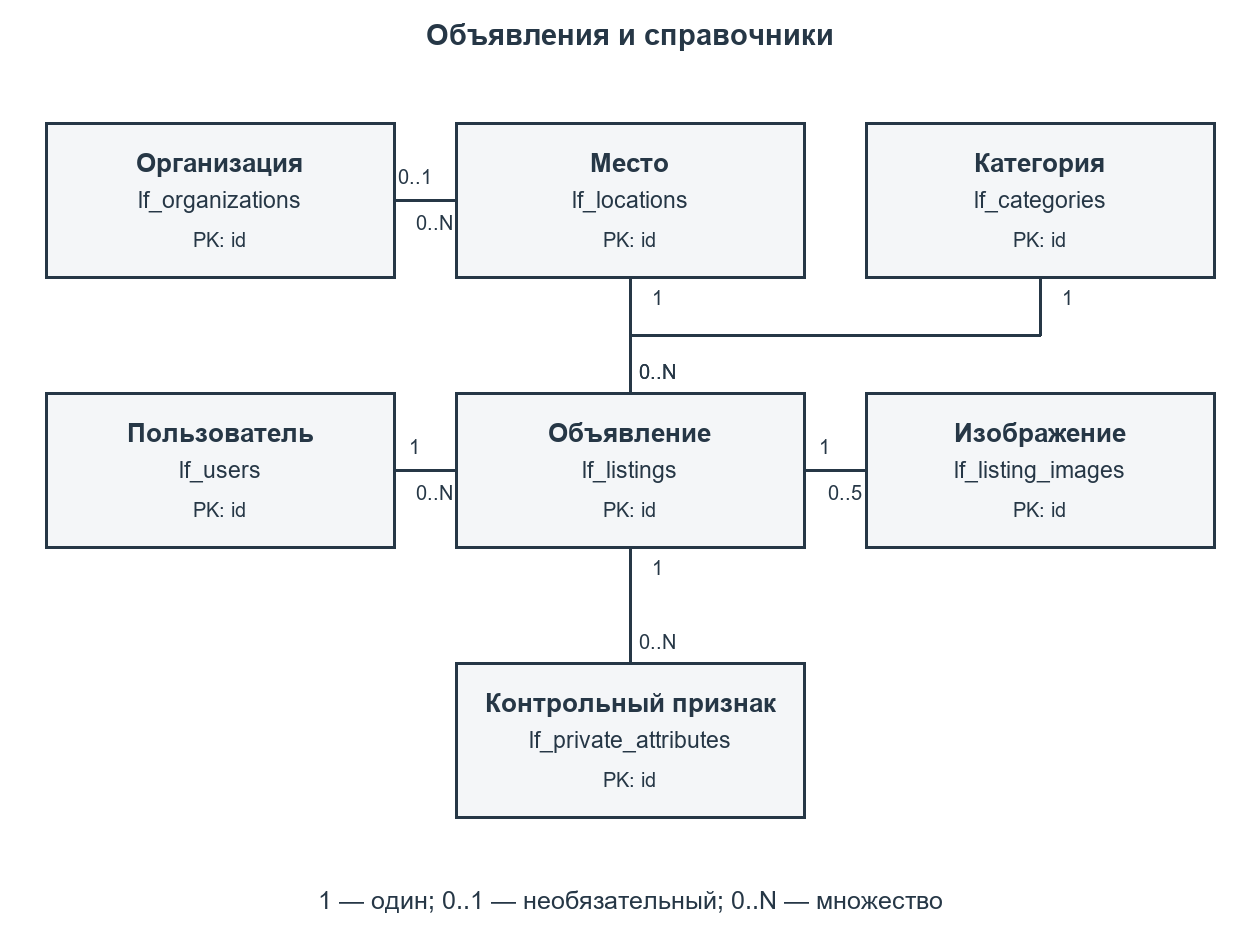
\includegraphics[width=\linewidth,height=0.82\textheight,keepaspectratio]{model/02_listings.png}
\caption*{Рисунок 8 — ER-модель: объявления и справочники}
\end{figure}
\FloatBarrier

\FloatBarrier
\begin{figure}[htbp]
\centering
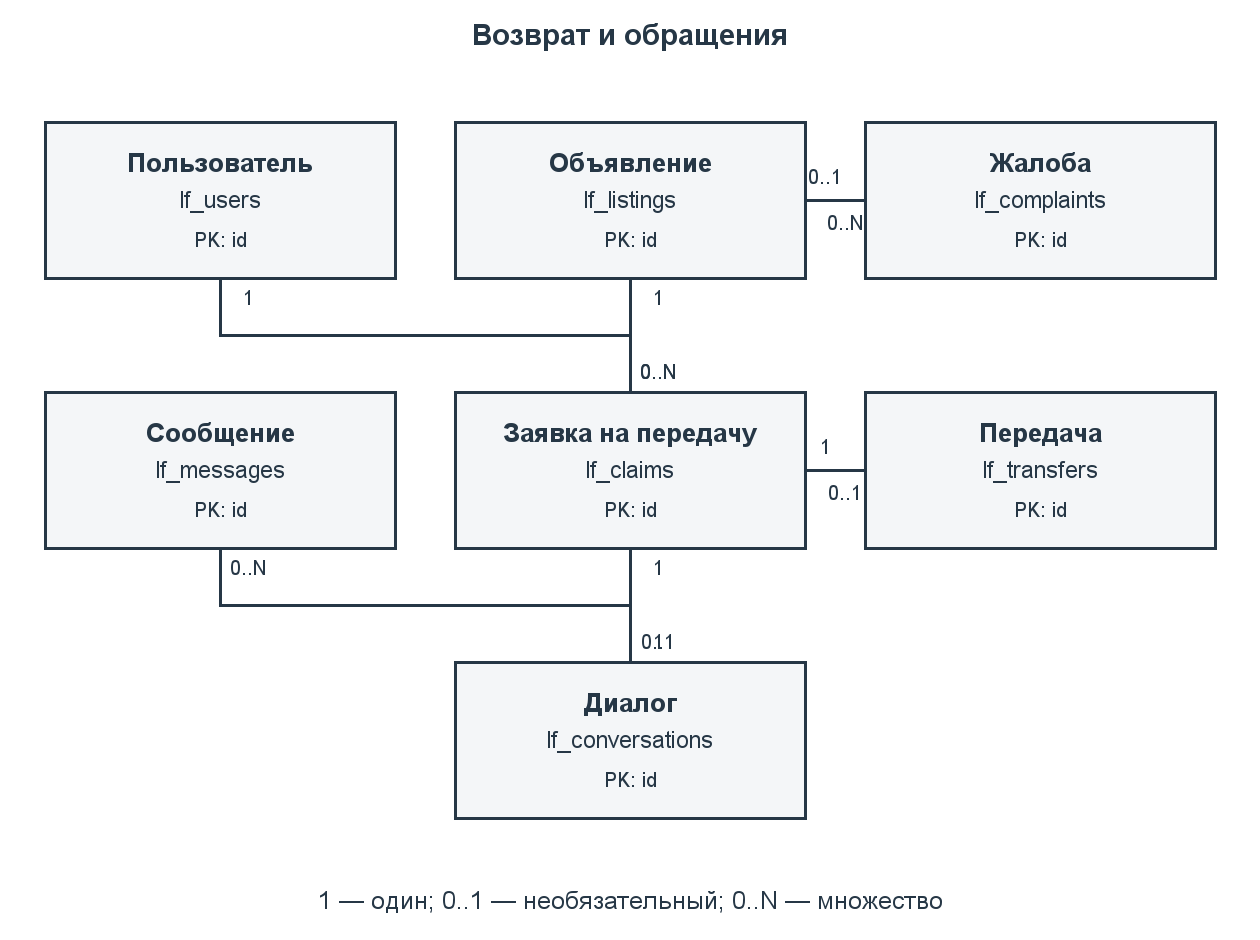
\includegraphics[width=\linewidth,height=0.82\textheight,keepaspectratio]{model/03_returns.png}
\caption*{Рисунок 9 — ER-модель: возврат и обращения}
\end{figure}
\FloatBarrier

\FloatBarrier
\begin{figure}[htbp]
\centering
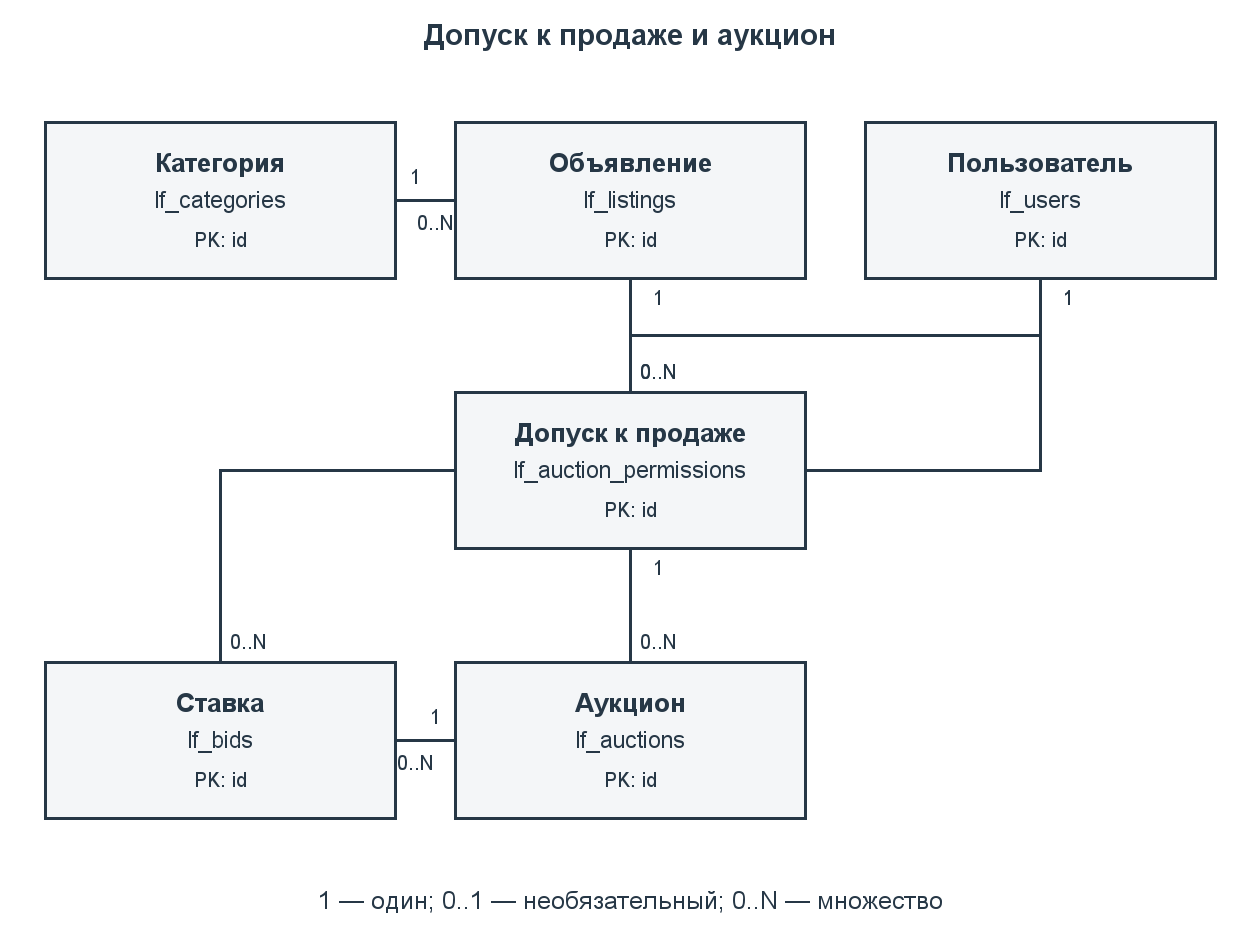
\includegraphics[width=\linewidth,height=0.82\textheight,keepaspectratio]{model/04_auctions.png}
\caption*{Рисунок 10 — ER-модель: аукционы}
\end{figure}
\FloatBarrier

\FloatBarrier
\begin{figure}[htbp]
\centering
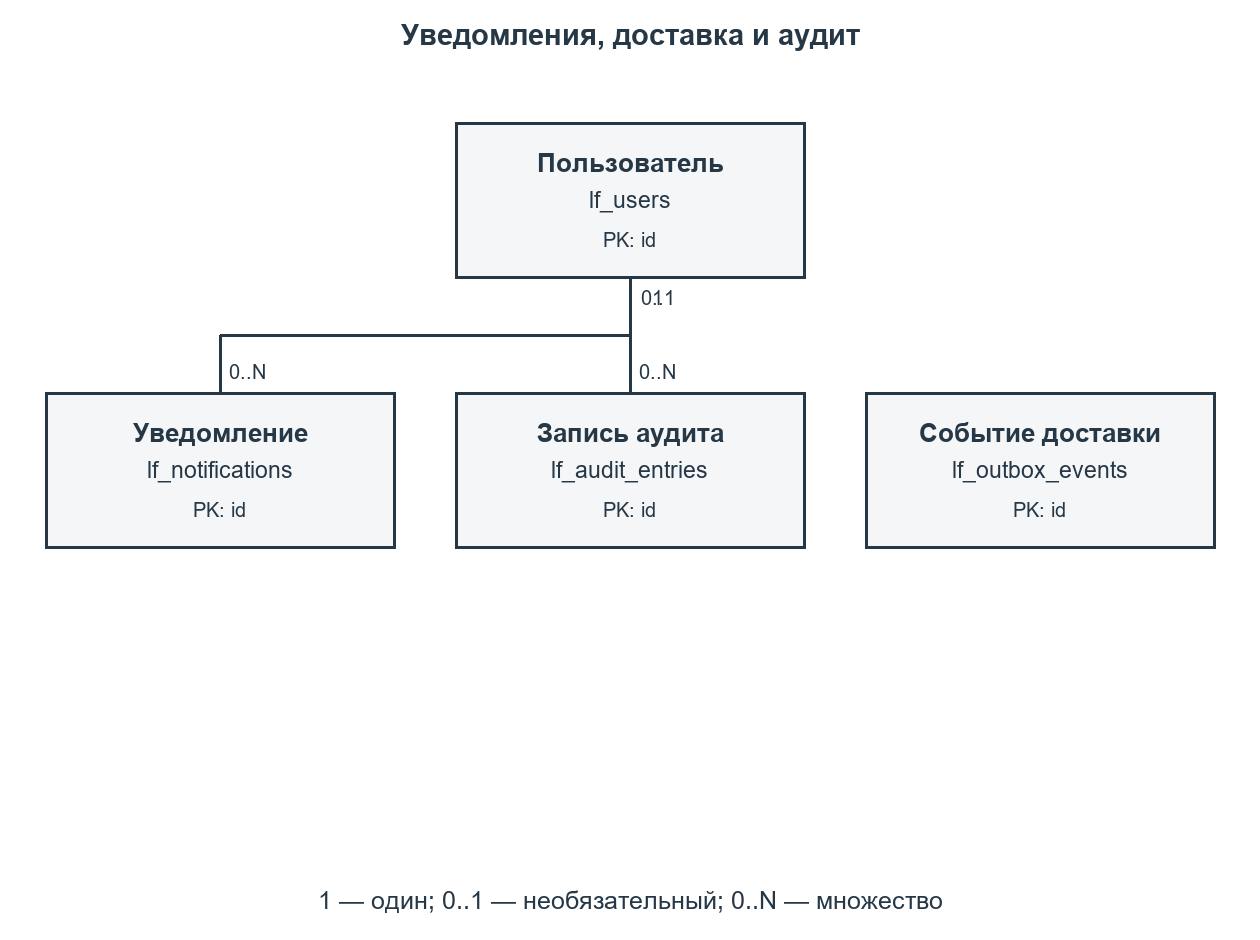
\includegraphics[width=\linewidth,height=0.82\textheight,keepaspectratio]{model/05_events.png}
\caption*{Рисунок 11 — ER-модель: уведомления, доставка и аудит}
\end{figure}
\FloatBarrier

\FloatBarrier
\begin{figure}[htbp]
\centering
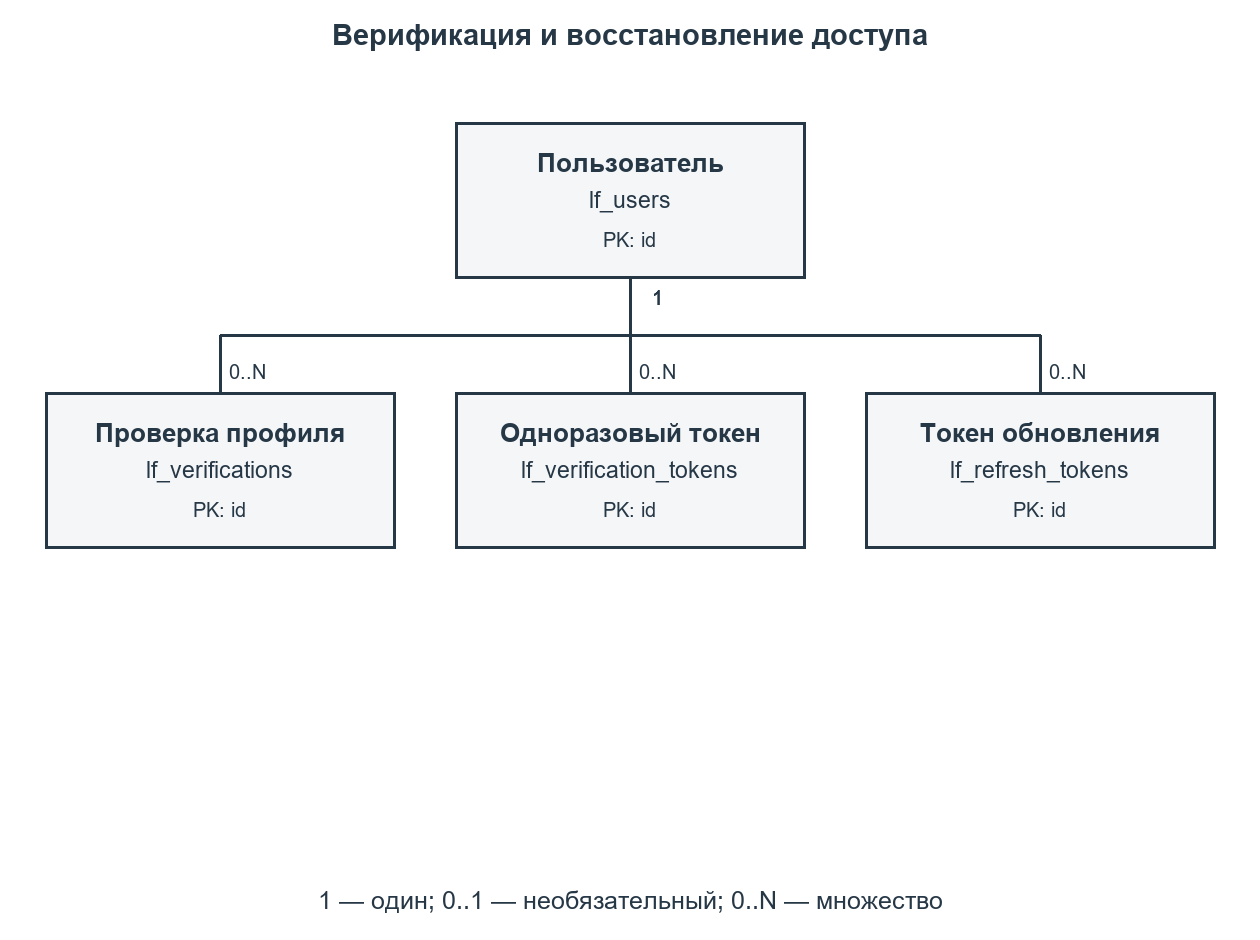
\includegraphics[width=\linewidth,height=0.82\textheight,keepaspectratio]{model/06_tokens.png}
\caption*{Рисунок 12 — ER-модель: верификация и токены}
\end{figure}
\FloatBarrier

Редактируемая концептуальная модель находится в docs/\allowbreak{}part2/\allowbreak{}model/\allowbreak{}er.mmd, полная даталогическая схема — в logical.mmd. Формат Mermaid поддерживает отображение ER-диаграмм и связей с ключами. Изображения каждого листа предоставлены в PNG и SVG.

\clearpage
\section{Даталогическая модель}

\FloatBarrier
\Needspace{6\baselineskip}
\subsection{Преобразование ER-модели}

Каждая сущность преобразована в таблицу Postgre\allowbreak{}SQL. Основные идентификаторы — bigint GENERATED BY DEFAULT AS IDENTITY; код роли является естественным ключом. Для ассоциации пользователей и ролей выбран составной ключ. Связи 1:N реализованы внешними ключами; для связей 1:0..1 добавлено UNIQUE: заявка — диалог, заявка — передача и заказ оплаты — период подписки.

Модель приведена к третьей нормальной форме. Атрибуты пользователя не копируются в объявления, диалоги и ставки. Сведения о категории, месте, организации и тарифе вынесены в справочники. Составной ключ назначения роли не содержит атрибутов, зависящих только от одной его части. Снимок суммы и длительности в заказе относится к самому заказу и необходим для сохранения условий оплаты, поэтому не заменяется ссылкой на текущие значения тарифа.

Время хранится в timestamptz. Начало события обязательно; event\_\allowbreak{}until задаётся только для интервала потери. Денежные значения используют numeric(12,2), без float. Закрытые признаки хранятся в lf\_\allowbreak{}private\_\allowbreak{}attributes и отсутствуют в публичном представлении. Файлы представлены ключами вложений закрытого локального каталога; бинарные данные не записываются в Postgre\allowbreak{}SQL. Технические JSON-поля применяются только в очереди событий и аудите, а связи предметной области остаются реляционными.

Циклическая связь аукциона и выигравшей ставки реализована составным внешним ключом (id, winner\_\allowbreak{}bid\_\allowbreak{}id) \ensuremath{\rightarrow} lf\_\allowbreak{}bids(auction\_\allowbreak{}id, id), отложенным до завершения транзакции. Победитель не может относиться к другому аукциону. Отложенная проверка резерва позволяет в одной транзакции согласовать заявку и изменить статус объявления. Физический столбец search\_\allowbreak{}vector является контролируемой избыточностью для поиска: Postgre\allowbreak{}SQL вычисляет его из текста объявления автоматически; в концептуальной нормализованной модели этот атрибут не требуется.

Словарь отношений сформирован из системного каталога Postgre\allowbreak{}SQL после установки на helios. Он отражает реально созданные типы, возможность NULL, первичные и внешние ключи. Отдельные частичные уникальные индексы описаны в разделе 13.

\FloatBarrier
\Needspace{6\baselineskip}
\subsection{Словарь отношений}

\FloatBarrier
\Needspace{6\baselineskip}
\subsubsection*{1. Допуск к продаже: lf\_\allowbreak{}auction\_\allowbreak{}permissions}

\begingroup
\setstretch{1}
\fontsize{11}{13}\selectfont
\setlength{\tablecontentwidth}{\dimexpr\linewidth-8\tabcolsep-5\arrayrulewidth\relax}
\begin{longtable}{|>{\RaggedRight\arraybackslash}p{0.38\tablecontentwidth}|>{\RaggedRight\arraybackslash}p{0.36\tablecontentwidth}|>{\RaggedRight\arraybackslash}p{0.11\tablecontentwidth}|>{\RaggedRight\arraybackslash}p{0.15\tablecontentwidth}|}
\hline
\textbf{Поле} & \textbf{Тип Postgre\allowbreak{}SQL} & \textbf{NULL} & \textbf{Ключ} \\ \hline
\endfirsthead
\textbf{Поле} & \textbf{Тип Postgre\allowbreak{}SQL} & \textbf{NULL} & \textbf{Ключ} \\ \hline
\endhead
\multicolumn{4}{r}{\footnotesize Продолжение на следующей странице} \\
\endfoot
\endlastfoot
id & bigint & Нет & PK \\ \hline
listing\_\allowbreak{}id & bigint & Нет & FK \\ \hline
applicant\_\allowbreak{}id & bigint & Нет & FK \\ \hline
basis & varchar(20) & Нет & — \\ \hline
evidence\_\allowbreak{}object\_\allowbreak{}key & varchar(240) & Нет & — \\ \hline
state & varchar(12) & Нет & — \\ \hline
moderator\_\allowbreak{}id & bigint & Да & FK \\ \hline
reviewed\_\allowbreak{}at & timestamptz & Да & — \\ \hline
reason & text & Да & — \\ \hline
created\_\allowbreak{}at & timestamptz & Нет & — \\ \hline
\end{longtable}
\endgroup

FOREIGN KEY (applicant\_\allowbreak{}id) REFERENCES lf\_\allowbreak{}users(id).

UNIQUE (id, listing\_\allowbreak{}id, applicant\_\allowbreak{}id).

FOREIGN KEY (listing\_\allowbreak{}id) REFERENCES lf\_\allowbreak{}listings(id).

FOREIGN KEY (moderator\_\allowbreak{}id) REFERENCES lf\_\allowbreak{}users(id).

PRIMARY KEY (id).

\FloatBarrier
\Needspace{6\baselineskip}
\subsubsection*{2. Аукцион: lf\_\allowbreak{}auctions}

\begingroup
\setstretch{1}
\fontsize{11}{13}\selectfont
\setlength{\tablecontentwidth}{\dimexpr\linewidth-8\tabcolsep-5\arrayrulewidth\relax}
\begin{longtable}{|>{\RaggedRight\arraybackslash}p{0.38\tablecontentwidth}|>{\RaggedRight\arraybackslash}p{0.36\tablecontentwidth}|>{\RaggedRight\arraybackslash}p{0.11\tablecontentwidth}|>{\RaggedRight\arraybackslash}p{0.15\tablecontentwidth}|}
\hline
\textbf{Поле} & \textbf{Тип Postgre\allowbreak{}SQL} & \textbf{NULL} & \textbf{Ключ} \\ \hline
\endfirsthead
\textbf{Поле} & \textbf{Тип Postgre\allowbreak{}SQL} & \textbf{NULL} & \textbf{Ключ} \\ \hline
\endhead
\multicolumn{4}{r}{\footnotesize Продолжение на следующей странице} \\
\endfoot
\endlastfoot
id & bigint & Нет & PK, FK \\ \hline
listing\_\allowbreak{}id & bigint & Нет & FK \\ \hline
seller\_\allowbreak{}id & bigint & Нет & FK \\ \hline
permission\_\allowbreak{}id & bigint & Нет & FK \\ \hline
starts\_\allowbreak{}at & timestamptz & Нет & — \\ \hline
ends\_\allowbreak{}at & timestamptz & Нет & — \\ \hline
start\_\allowbreak{}price & numeric(12,2) & Нет & — \\ \hline
bid\_\allowbreak{}step & numeric(12,2) & Нет & — \\ \hline
state & varchar(12) & Нет & — \\ \hline
winner\_\allowbreak{}bid\_\allowbreak{}id & bigint & Да & FK \\ \hline
closed\_\allowbreak{}at & timestamptz & Да & — \\ \hline
\end{longtable}
\endgroup

FOREIGN KEY (listing\_\allowbreak{}id) REFERENCES lf\_\allowbreak{}listings(id).

FOREIGN KEY (permission\_\allowbreak{}id, listing\_\allowbreak{}id, seller\_\allowbreak{}id) REFERENCES lf\_\allowbreak{}auction\_\allowbreak{}permissions(id, listing\_\allowbreak{}id, applicant\_\allowbreak{}id).

PRIMARY KEY (id).

FOREIGN KEY (seller\_\allowbreak{}id) REFERENCES lf\_\allowbreak{}users(id).

FOREIGN KEY (id, winner\_\allowbreak{}bid\_\allowbreak{}id) REFERENCES lf\_\allowbreak{}bids(auction\_\allowbreak{}id, id) DEFERRABLE INITIALLY DEFERRED.

\FloatBarrier
\Needspace{6\baselineskip}
\subsubsection*{3. Запись аудита: lf\_\allowbreak{}audit\_\allowbreak{}entries}

\begingroup
\setstretch{1}
\fontsize{11}{13}\selectfont
\setlength{\tablecontentwidth}{\dimexpr\linewidth-8\tabcolsep-5\arrayrulewidth\relax}
\begin{longtable}{|>{\RaggedRight\arraybackslash}p{0.38\tablecontentwidth}|>{\RaggedRight\arraybackslash}p{0.36\tablecontentwidth}|>{\RaggedRight\arraybackslash}p{0.11\tablecontentwidth}|>{\RaggedRight\arraybackslash}p{0.15\tablecontentwidth}|}
\hline
\textbf{Поле} & \textbf{Тип Postgre\allowbreak{}SQL} & \textbf{NULL} & \textbf{Ключ} \\ \hline
\endfirsthead
\textbf{Поле} & \textbf{Тип Postgre\allowbreak{}SQL} & \textbf{NULL} & \textbf{Ключ} \\ \hline
\endhead
\multicolumn{4}{r}{\footnotesize Продолжение на следующей странице} \\
\endfoot
\endlastfoot
id & bigint & Нет & PK \\ \hline
actor\_\allowbreak{}id & bigint & Да & FK \\ \hline
action & varchar(80) & Нет & — \\ \hline
entity\_\allowbreak{}table & varchar(80) & Нет & — \\ \hline
entity\_\allowbreak{}id & bigint & Нет & — \\ \hline
details & jsonb & Нет & — \\ \hline
created\_\allowbreak{}at & timestamptz & Нет & — \\ \hline
\end{longtable}
\endgroup

FOREIGN KEY (actor\_\allowbreak{}id) REFERENCES lf\_\allowbreak{}users(id).

PRIMARY KEY (id).

\FloatBarrier
\Needspace{6\baselineskip}
\subsubsection*{4. Ставка: lf\_\allowbreak{}bids}

\begingroup
\setstretch{1}
\fontsize{11}{13}\selectfont
\setlength{\tablecontentwidth}{\dimexpr\linewidth-8\tabcolsep-5\arrayrulewidth\relax}
\begin{longtable}{|>{\RaggedRight\arraybackslash}p{0.38\tablecontentwidth}|>{\RaggedRight\arraybackslash}p{0.36\tablecontentwidth}|>{\RaggedRight\arraybackslash}p{0.11\tablecontentwidth}|>{\RaggedRight\arraybackslash}p{0.15\tablecontentwidth}|}
\hline
\textbf{Поле} & \textbf{Тип Postgre\allowbreak{}SQL} & \textbf{NULL} & \textbf{Ключ} \\ \hline
\endfirsthead
\textbf{Поле} & \textbf{Тип Postgre\allowbreak{}SQL} & \textbf{NULL} & \textbf{Ключ} \\ \hline
\endhead
\multicolumn{4}{r}{\footnotesize Продолжение на следующей странице} \\
\endfoot
\endlastfoot
id & bigint & Нет & PK \\ \hline
auction\_\allowbreak{}id & bigint & Нет & FK \\ \hline
bidder\_\allowbreak{}id & bigint & Нет & FK \\ \hline
request\_\allowbreak{}key & uuid & Нет & — \\ \hline
amount & numeric(12,2) & Нет & — \\ \hline
placed\_\allowbreak{}at & timestamptz & Нет & — \\ \hline
\end{longtable}
\endgroup

FOREIGN KEY (auction\_\allowbreak{}id) REFERENCES lf\_\allowbreak{}auctions(id).

UNIQUE (auction\_\allowbreak{}id, id).

FOREIGN KEY (bidder\_\allowbreak{}id) REFERENCES lf\_\allowbreak{}users(id).

PRIMARY KEY (id).

UNIQUE (request\_\allowbreak{}key).

\FloatBarrier
\Needspace{6\baselineskip}
\subsubsection*{5. Категория: lf\_\allowbreak{}categories}

\begingroup
\setstretch{1}
\fontsize{11}{13}\selectfont
\setlength{\tablecontentwidth}{\dimexpr\linewidth-8\tabcolsep-5\arrayrulewidth\relax}
\begin{longtable}{|>{\RaggedRight\arraybackslash}p{0.38\tablecontentwidth}|>{\RaggedRight\arraybackslash}p{0.36\tablecontentwidth}|>{\RaggedRight\arraybackslash}p{0.11\tablecontentwidth}|>{\RaggedRight\arraybackslash}p{0.15\tablecontentwidth}|}
\hline
\textbf{Поле} & \textbf{Тип Postgre\allowbreak{}SQL} & \textbf{NULL} & \textbf{Ключ} \\ \hline
\endfirsthead
\textbf{Поле} & \textbf{Тип Postgre\allowbreak{}SQL} & \textbf{NULL} & \textbf{Ключ} \\ \hline
\endhead
\multicolumn{4}{r}{\footnotesize Продолжение на следующей странице} \\
\endfoot
\endlastfoot
id & bigint & Нет & PK \\ \hline
name & varchar(80) & Нет & — \\ \hline
auction\_\allowbreak{}allowed & boolean & Нет & — \\ \hline
\end{longtable}
\endgroup

UNIQUE (name).

PRIMARY KEY (id).

\FloatBarrier
\Needspace{6\baselineskip}
\subsubsection*{6. Заявка на передачу: lf\_\allowbreak{}claims}

\begingroup
\setstretch{1}
\fontsize{11}{13}\selectfont
\setlength{\tablecontentwidth}{\dimexpr\linewidth-8\tabcolsep-5\arrayrulewidth\relax}
\begin{longtable}{|>{\RaggedRight\arraybackslash}p{0.38\tablecontentwidth}|>{\RaggedRight\arraybackslash}p{0.36\tablecontentwidth}|>{\RaggedRight\arraybackslash}p{0.11\tablecontentwidth}|>{\RaggedRight\arraybackslash}p{0.15\tablecontentwidth}|}
\hline
\textbf{Поле} & \textbf{Тип Postgre\allowbreak{}SQL} & \textbf{NULL} & \textbf{Ключ} \\ \hline
\endfirsthead
\textbf{Поле} & \textbf{Тип Postgre\allowbreak{}SQL} & \textbf{NULL} & \textbf{Ключ} \\ \hline
\endhead
\multicolumn{4}{r}{\footnotesize Продолжение на следующей странице} \\
\endfoot
\endlastfoot
id & bigint & Нет & PK \\ \hline
listing\_\allowbreak{}id & bigint & Нет & FK \\ \hline
claimant\_\allowbreak{}id & bigint & Нет & FK \\ \hline
evidence & text & Нет & — \\ \hline
state & varchar(12) & Нет & — \\ \hline
created\_\allowbreak{}at & timestamptz & Нет & — \\ \hline
auction\_\allowbreak{}id & bigint & Да & FK \\ \hline
\end{longtable}
\endgroup

FOREIGN KEY (auction\_\allowbreak{}id) REFERENCES lf\_\allowbreak{}auctions(id).

UNIQUE (auction\_\allowbreak{}id).

FOREIGN KEY (claimant\_\allowbreak{}id) REFERENCES lf\_\allowbreak{}users(id).

UNIQUE (id, listing\_\allowbreak{}id).

FOREIGN KEY (listing\_\allowbreak{}id) REFERENCES lf\_\allowbreak{}listings(id).

PRIMARY KEY (id).

\FloatBarrier
\Needspace{6\baselineskip}
\subsubsection*{7. Жалоба: lf\_\allowbreak{}complaints}

\begingroup
\setstretch{1}
\fontsize{11}{13}\selectfont
\setlength{\tablecontentwidth}{\dimexpr\linewidth-8\tabcolsep-5\arrayrulewidth\relax}
\begin{longtable}{|>{\RaggedRight\arraybackslash}p{0.38\tablecontentwidth}|>{\RaggedRight\arraybackslash}p{0.36\tablecontentwidth}|>{\RaggedRight\arraybackslash}p{0.11\tablecontentwidth}|>{\RaggedRight\arraybackslash}p{0.15\tablecontentwidth}|}
\hline
\textbf{Поле} & \textbf{Тип Postgre\allowbreak{}SQL} & \textbf{NULL} & \textbf{Ключ} \\ \hline
\endfirsthead
\textbf{Поле} & \textbf{Тип Postgre\allowbreak{}SQL} & \textbf{NULL} & \textbf{Ключ} \\ \hline
\endhead
\multicolumn{4}{r}{\footnotesize Продолжение на следующей странице} \\
\endfoot
\endlastfoot
id & bigint & Нет & PK \\ \hline
reporter\_\allowbreak{}id & bigint & Нет & FK \\ \hline
listing\_\allowbreak{}id & bigint & Да & FK \\ \hline
reported\_\allowbreak{}user\_\allowbreak{}id & bigint & Да & FK \\ \hline
reason & text & Нет & — \\ \hline
state & varchar(12) & Нет & — \\ \hline
moderator\_\allowbreak{}id & bigint & Да & FK \\ \hline
resolution & text & Да & — \\ \hline
created\_\allowbreak{}at & timestamptz & Нет & — \\ \hline
\end{longtable}
\endgroup

FOREIGN KEY (listing\_\allowbreak{}id) REFERENCES lf\_\allowbreak{}listings(id).

FOREIGN KEY (moderator\_\allowbreak{}id) REFERENCES lf\_\allowbreak{}users(id).

PRIMARY KEY (id).

FOREIGN KEY (reported\_\allowbreak{}user\_\allowbreak{}id) REFERENCES lf\_\allowbreak{}users(id).

FOREIGN KEY (reporter\_\allowbreak{}id) REFERENCES lf\_\allowbreak{}users(id).

\FloatBarrier
\Needspace{6\baselineskip}
\subsubsection*{8. Диалог: lf\_\allowbreak{}conversations}

\begingroup
\setstretch{1}
\fontsize{11}{13}\selectfont
\setlength{\tablecontentwidth}{\dimexpr\linewidth-8\tabcolsep-5\arrayrulewidth\relax}
\begin{longtable}{|>{\RaggedRight\arraybackslash}p{0.38\tablecontentwidth}|>{\RaggedRight\arraybackslash}p{0.36\tablecontentwidth}|>{\RaggedRight\arraybackslash}p{0.11\tablecontentwidth}|>{\RaggedRight\arraybackslash}p{0.15\tablecontentwidth}|}
\hline
\textbf{Поле} & \textbf{Тип Postgre\allowbreak{}SQL} & \textbf{NULL} & \textbf{Ключ} \\ \hline
\endfirsthead
\textbf{Поле} & \textbf{Тип Postgre\allowbreak{}SQL} & \textbf{NULL} & \textbf{Ключ} \\ \hline
\endhead
\multicolumn{4}{r}{\footnotesize Продолжение на следующей странице} \\
\endfoot
\endlastfoot
id & bigint & Нет & PK \\ \hline
claim\_\allowbreak{}id & bigint & Нет & FK \\ \hline
created\_\allowbreak{}at & timestamptz & Нет & — \\ \hline
\end{longtable}
\endgroup

FOREIGN KEY (claim\_\allowbreak{}id) REFERENCES lf\_\allowbreak{}claims(id).

UNIQUE (claim\_\allowbreak{}id).

PRIMARY KEY (id).

\FloatBarrier
\Needspace{6\baselineskip}
\subsubsection*{9. Изображение: lf\_\allowbreak{}listing\_\allowbreak{}images}

\begingroup
\setstretch{1}
\fontsize{11}{13}\selectfont
\setlength{\tablecontentwidth}{\dimexpr\linewidth-8\tabcolsep-5\arrayrulewidth\relax}
\begin{longtable}{|>{\RaggedRight\arraybackslash}p{0.38\tablecontentwidth}|>{\RaggedRight\arraybackslash}p{0.36\tablecontentwidth}|>{\RaggedRight\arraybackslash}p{0.11\tablecontentwidth}|>{\RaggedRight\arraybackslash}p{0.15\tablecontentwidth}|}
\hline
\textbf{Поле} & \textbf{Тип Postgre\allowbreak{}SQL} & \textbf{NULL} & \textbf{Ключ} \\ \hline
\endfirsthead
\textbf{Поле} & \textbf{Тип Postgre\allowbreak{}SQL} & \textbf{NULL} & \textbf{Ключ} \\ \hline
\endhead
\multicolumn{4}{r}{\footnotesize Продолжение на следующей странице} \\
\endfoot
\endlastfoot
id & bigint & Нет & PK \\ \hline
listing\_\allowbreak{}id & bigint & Нет & FK \\ \hline
object\_\allowbreak{}key & varchar(240) & Нет & — \\ \hline
media\_\allowbreak{}type & varchar(20) & Нет & — \\ \hline
size\_\allowbreak{}bytes & integer & Нет & — \\ \hline
position & smallint & Нет & — \\ \hline
\end{longtable}
\endgroup

FOREIGN KEY (listing\_\allowbreak{}id) REFERENCES lf\_\allowbreak{}listings(id) ON DELETE CASCADE.

UNIQUE (listing\_\allowbreak{}id, "position").

UNIQUE (object\_\allowbreak{}key).

PRIMARY KEY (id).

\FloatBarrier
\Needspace{6\baselineskip}
\subsubsection*{10. Объявление: lf\_\allowbreak{}listings}

\begingroup
\setstretch{1}
\fontsize{11}{13}\selectfont
\setlength{\tablecontentwidth}{\dimexpr\linewidth-8\tabcolsep-5\arrayrulewidth\relax}
\begin{longtable}{|>{\RaggedRight\arraybackslash}p{0.38\tablecontentwidth}|>{\RaggedRight\arraybackslash}p{0.36\tablecontentwidth}|>{\RaggedRight\arraybackslash}p{0.11\tablecontentwidth}|>{\RaggedRight\arraybackslash}p{0.15\tablecontentwidth}|}
\hline
\textbf{Поле} & \textbf{Тип Postgre\allowbreak{}SQL} & \textbf{NULL} & \textbf{Ключ} \\ \hline
\endfirsthead
\textbf{Поле} & \textbf{Тип Postgre\allowbreak{}SQL} & \textbf{NULL} & \textbf{Ключ} \\ \hline
\endhead
\multicolumn{4}{r}{\footnotesize Продолжение на следующей странице} \\
\endfoot
\endlastfoot
id & bigint & Нет & PK \\ \hline
author\_\allowbreak{}id & bigint & Нет & FK \\ \hline
category\_\allowbreak{}id & bigint & Нет & FK \\ \hline
location\_\allowbreak{}id & bigint & Нет & FK \\ \hline
kind & varchar(5) & Нет & — \\ \hline
title & varchar(120) & Нет & — \\ \hline
description & text & Нет & — \\ \hline
event\_\allowbreak{}at & timestamptz & Нет & — \\ \hline
event\_\allowbreak{}until & timestamptz & Да & — \\ \hline
state & varchar(12) & Нет & — \\ \hline
custodian\_\allowbreak{}org\_\allowbreak{}id & bigint & Да & FK \\ \hline
official\_\allowbreak{}reported\_\allowbreak{}at & timestamptz & Да & — \\ \hline
moderator\_\allowbreak{}id & bigint & Да & FK \\ \hline
moderated\_\allowbreak{}at & timestamptz & Да & — \\ \hline
created\_\allowbreak{}at & timestamptz & Нет & — \\ \hline
search\_\allowbreak{}vector & tsvector & Да & — \\ \hline
\end{longtable}
\endgroup

FOREIGN KEY (author\_\allowbreak{}id) REFERENCES lf\_\allowbreak{}users(id).

FOREIGN KEY (category\_\allowbreak{}id) REFERENCES lf\_\allowbreak{}categories(id).

FOREIGN KEY (custodian\_\allowbreak{}org\_\allowbreak{}id) REFERENCES lf\_\allowbreak{}organizations(id).

FOREIGN KEY (location\_\allowbreak{}id) REFERENCES lf\_\allowbreak{}locations(id).

FOREIGN KEY (moderator\_\allowbreak{}id) REFERENCES lf\_\allowbreak{}users(id).

PRIMARY KEY (id).

\FloatBarrier
\Needspace{6\baselineskip}
\subsubsection*{11. Место: lf\_\allowbreak{}locations}

\begingroup
\setstretch{1}
\fontsize{11}{13}\selectfont
\setlength{\tablecontentwidth}{\dimexpr\linewidth-8\tabcolsep-5\arrayrulewidth\relax}
\begin{longtable}{|>{\RaggedRight\arraybackslash}p{0.38\tablecontentwidth}|>{\RaggedRight\arraybackslash}p{0.36\tablecontentwidth}|>{\RaggedRight\arraybackslash}p{0.11\tablecontentwidth}|>{\RaggedRight\arraybackslash}p{0.15\tablecontentwidth}|}
\hline
\textbf{Поле} & \textbf{Тип Postgre\allowbreak{}SQL} & \textbf{NULL} & \textbf{Ключ} \\ \hline
\endfirsthead
\textbf{Поле} & \textbf{Тип Postgre\allowbreak{}SQL} & \textbf{NULL} & \textbf{Ключ} \\ \hline
\endhead
\multicolumn{4}{r}{\footnotesize Продолжение на следующей странице} \\
\endfoot
\endlastfoot
id & bigint & Нет & PK \\ \hline
city & varchar(80) & Нет & — \\ \hline
description & varchar(240) & Нет & — \\ \hline
latitude & numeric(9,6) & Да & — \\ \hline
longitude & numeric(9,6) & Да & — \\ \hline
metro\_\allowbreak{}station & varchar(100) & Да & — \\ \hline
organization\_\allowbreak{}id & bigint & Да & FK \\ \hline
\end{longtable}
\endgroup

FOREIGN KEY (organization\_\allowbreak{}id) REFERENCES lf\_\allowbreak{}organizations(id).

PRIMARY KEY (id).

\FloatBarrier
\Needspace{6\baselineskip}
\subsubsection*{12. Сообщение: lf\_\allowbreak{}messages}

\begingroup
\setstretch{1}
\fontsize{11}{13}\selectfont
\setlength{\tablecontentwidth}{\dimexpr\linewidth-8\tabcolsep-5\arrayrulewidth\relax}
\begin{longtable}{|>{\RaggedRight\arraybackslash}p{0.38\tablecontentwidth}|>{\RaggedRight\arraybackslash}p{0.36\tablecontentwidth}|>{\RaggedRight\arraybackslash}p{0.11\tablecontentwidth}|>{\RaggedRight\arraybackslash}p{0.15\tablecontentwidth}|}
\hline
\textbf{Поле} & \textbf{Тип Postgre\allowbreak{}SQL} & \textbf{NULL} & \textbf{Ключ} \\ \hline
\endfirsthead
\textbf{Поле} & \textbf{Тип Postgre\allowbreak{}SQL} & \textbf{NULL} & \textbf{Ключ} \\ \hline
\endhead
\multicolumn{4}{r}{\footnotesize Продолжение на следующей странице} \\
\endfoot
\endlastfoot
id & bigint & Нет & PK \\ \hline
conversation\_\allowbreak{}id & bigint & Нет & FK \\ \hline
sender\_\allowbreak{}id & bigint & Нет & FK \\ \hline
body & text & Нет & — \\ \hline
sent\_\allowbreak{}at & timestamptz & Нет & — \\ \hline
\end{longtable}
\endgroup

FOREIGN KEY (conversation\_\allowbreak{}id) REFERENCES lf\_\allowbreak{}conversations(id).

PRIMARY KEY (id).

FOREIGN KEY (sender\_\allowbreak{}id) REFERENCES lf\_\allowbreak{}users(id).

\FloatBarrier
\Needspace{6\baselineskip}
\subsubsection*{13. Уведомление: lf\_\allowbreak{}notifications}

\begingroup
\setstretch{1}
\fontsize{11}{13}\selectfont
\setlength{\tablecontentwidth}{\dimexpr\linewidth-8\tabcolsep-5\arrayrulewidth\relax}
\begin{longtable}{|>{\RaggedRight\arraybackslash}p{0.38\tablecontentwidth}|>{\RaggedRight\arraybackslash}p{0.36\tablecontentwidth}|>{\RaggedRight\arraybackslash}p{0.11\tablecontentwidth}|>{\RaggedRight\arraybackslash}p{0.15\tablecontentwidth}|}
\hline
\textbf{Поле} & \textbf{Тип Postgre\allowbreak{}SQL} & \textbf{NULL} & \textbf{Ключ} \\ \hline
\endfirsthead
\textbf{Поле} & \textbf{Тип Postgre\allowbreak{}SQL} & \textbf{NULL} & \textbf{Ключ} \\ \hline
\endhead
\multicolumn{4}{r}{\footnotesize Продолжение на следующей странице} \\
\endfoot
\endlastfoot
id & bigint & Нет & PK \\ \hline
user\_\allowbreak{}id & bigint & Нет & FK \\ \hline
kind & varchar(40) & Нет & — \\ \hline
body & text & Нет & — \\ \hline
read\_\allowbreak{}at & timestamptz & Да & — \\ \hline
created\_\allowbreak{}at & timestamptz & Нет & — \\ \hline
\end{longtable}
\endgroup

PRIMARY KEY (id).

FOREIGN KEY (user\_\allowbreak{}id) REFERENCES lf\_\allowbreak{}users(id).

\FloatBarrier
\Needspace{6\baselineskip}
\subsubsection*{14. Организация: lf\_\allowbreak{}organizations}

\begingroup
\setstretch{1}
\fontsize{11}{13}\selectfont
\setlength{\tablecontentwidth}{\dimexpr\linewidth-8\tabcolsep-5\arrayrulewidth\relax}
\begin{longtable}{|>{\RaggedRight\arraybackslash}p{0.38\tablecontentwidth}|>{\RaggedRight\arraybackslash}p{0.36\tablecontentwidth}|>{\RaggedRight\arraybackslash}p{0.11\tablecontentwidth}|>{\RaggedRight\arraybackslash}p{0.15\tablecontentwidth}|}
\hline
\textbf{Поле} & \textbf{Тип Postgre\allowbreak{}SQL} & \textbf{NULL} & \textbf{Ключ} \\ \hline
\endfirsthead
\textbf{Поле} & \textbf{Тип Postgre\allowbreak{}SQL} & \textbf{NULL} & \textbf{Ключ} \\ \hline
\endhead
\multicolumn{4}{r}{\footnotesize Продолжение на следующей странице} \\
\endfoot
\endlastfoot
id & bigint & Нет & PK \\ \hline
name & varchar(160) & Нет & — \\ \hline
phone & varchar(40) & Нет & — \\ \hline
address & text & Да & — \\ \hline
instructions & text & Нет & — \\ \hline
source\_\allowbreak{}url & text & Нет & — \\ \hline
verified\_\allowbreak{}on & date & Нет & — \\ \hline
\end{longtable}
\endgroup

UNIQUE (name).

PRIMARY KEY (id).

\FloatBarrier
\Needspace{6\baselineskip}
\subsubsection*{15. Событие доставки: lf\_\allowbreak{}outbox\_\allowbreak{}events}

\begingroup
\setstretch{1}
\fontsize{11}{13}\selectfont
\setlength{\tablecontentwidth}{\dimexpr\linewidth-8\tabcolsep-5\arrayrulewidth\relax}
\begin{longtable}{|>{\RaggedRight\arraybackslash}p{0.38\tablecontentwidth}|>{\RaggedRight\arraybackslash}p{0.36\tablecontentwidth}|>{\RaggedRight\arraybackslash}p{0.11\tablecontentwidth}|>{\RaggedRight\arraybackslash}p{0.15\tablecontentwidth}|}
\hline
\textbf{Поле} & \textbf{Тип Postgre\allowbreak{}SQL} & \textbf{NULL} & \textbf{Ключ} \\ \hline
\endfirsthead
\textbf{Поле} & \textbf{Тип Postgre\allowbreak{}SQL} & \textbf{NULL} & \textbf{Ключ} \\ \hline
\endhead
\multicolumn{4}{r}{\footnotesize Продолжение на следующей странице} \\
\endfoot
\endlastfoot
id & bigint & Нет & PK \\ \hline
kind & varchar(40) & Нет & — \\ \hline
aggregate\_\allowbreak{}id & bigint & Нет & — \\ \hline
payload & jsonb & Нет & — \\ \hline
attempts & integer & Нет & — \\ \hline
next\_\allowbreak{}attempt\_\allowbreak{}at & timestamptz & Нет & — \\ \hline
delivered\_\allowbreak{}at & timestamptz & Да & — \\ \hline
created\_\allowbreak{}at & timestamptz & Нет & — \\ \hline
\end{longtable}
\endgroup

PRIMARY KEY (id).

\FloatBarrier
\Needspace{6\baselineskip}
\subsubsection*{16. Событие оплаты: lf\_\allowbreak{}payment\_\allowbreak{}events}

\begingroup
\setstretch{1}
\fontsize{11}{13}\selectfont
\setlength{\tablecontentwidth}{\dimexpr\linewidth-8\tabcolsep-5\arrayrulewidth\relax}
\begin{longtable}{|>{\RaggedRight\arraybackslash}p{0.38\tablecontentwidth}|>{\RaggedRight\arraybackslash}p{0.36\tablecontentwidth}|>{\RaggedRight\arraybackslash}p{0.11\tablecontentwidth}|>{\RaggedRight\arraybackslash}p{0.15\tablecontentwidth}|}
\hline
\textbf{Поле} & \textbf{Тип Postgre\allowbreak{}SQL} & \textbf{NULL} & \textbf{Ключ} \\ \hline
\endfirsthead
\textbf{Поле} & \textbf{Тип Postgre\allowbreak{}SQL} & \textbf{NULL} & \textbf{Ключ} \\ \hline
\endhead
\multicolumn{4}{r}{\footnotesize Продолжение на следующей странице} \\
\endfoot
\endlastfoot
provider\_\allowbreak{}event\_\allowbreak{}id & varchar(100) & Нет & PK \\ \hline
order\_\allowbreak{}id & bigint & Нет & FK \\ \hline
amount & numeric(12,2) & Нет & — \\ \hline
currency & char(3) & Нет & — \\ \hline
received\_\allowbreak{}at & timestamptz & Нет & — \\ \hline
\end{longtable}
\endgroup

FOREIGN KEY (order\_\allowbreak{}id) REFERENCES lf\_\allowbreak{}payment\_\allowbreak{}orders(id).

PRIMARY KEY (provider\_\allowbreak{}event\_\allowbreak{}id).

\FloatBarrier
\Needspace{6\baselineskip}
\subsubsection*{17. Заказ оплаты: lf\_\allowbreak{}payment\_\allowbreak{}orders}

\begingroup
\setstretch{1}
\fontsize{11}{13}\selectfont
\setlength{\tablecontentwidth}{\dimexpr\linewidth-8\tabcolsep-5\arrayrulewidth\relax}
\begin{longtable}{|>{\RaggedRight\arraybackslash}p{0.38\tablecontentwidth}|>{\RaggedRight\arraybackslash}p{0.36\tablecontentwidth}|>{\RaggedRight\arraybackslash}p{0.11\tablecontentwidth}|>{\RaggedRight\arraybackslash}p{0.15\tablecontentwidth}|}
\hline
\textbf{Поле} & \textbf{Тип Postgre\allowbreak{}SQL} & \textbf{NULL} & \textbf{Ключ} \\ \hline
\endfirsthead
\textbf{Поле} & \textbf{Тип Postgre\allowbreak{}SQL} & \textbf{NULL} & \textbf{Ключ} \\ \hline
\endhead
\multicolumn{4}{r}{\footnotesize Продолжение на следующей странице} \\
\endfoot
\endlastfoot
id & bigint & Нет & PK \\ \hline
user\_\allowbreak{}id & bigint & Нет & FK \\ \hline
tariff\_\allowbreak{}id & bigint & Нет & FK \\ \hline
request\_\allowbreak{}key & uuid & Нет & — \\ \hline
amount & numeric(12,2) & Нет & — \\ \hline
duration\_\allowbreak{}days & integer & Нет & — \\ \hline
currency & char(3) & Нет & — \\ \hline
state & varchar(12) & Нет & — \\ \hline
created\_\allowbreak{}at & timestamptz & Нет & — \\ \hline
paid\_\allowbreak{}at & timestamptz & Да & — \\ \hline
\end{longtable}
\endgroup

PRIMARY KEY (id).

UNIQUE (request\_\allowbreak{}key).

FOREIGN KEY (tariff\_\allowbreak{}id) REFERENCES lf\_\allowbreak{}tariffs(id).

FOREIGN KEY (user\_\allowbreak{}id) REFERENCES lf\_\allowbreak{}users(id).

\FloatBarrier
\Needspace{6\baselineskip}
\subsubsection*{18. Контрольный признак: lf\_\allowbreak{}private\_\allowbreak{}attributes}

\begingroup
\setstretch{1}
\fontsize{11}{13}\selectfont
\setlength{\tablecontentwidth}{\dimexpr\linewidth-8\tabcolsep-5\arrayrulewidth\relax}
\begin{longtable}{|>{\RaggedRight\arraybackslash}p{0.38\tablecontentwidth}|>{\RaggedRight\arraybackslash}p{0.36\tablecontentwidth}|>{\RaggedRight\arraybackslash}p{0.11\tablecontentwidth}|>{\RaggedRight\arraybackslash}p{0.15\tablecontentwidth}|}
\hline
\textbf{Поле} & \textbf{Тип Postgre\allowbreak{}SQL} & \textbf{NULL} & \textbf{Ключ} \\ \hline
\endfirsthead
\textbf{Поле} & \textbf{Тип Postgre\allowbreak{}SQL} & \textbf{NULL} & \textbf{Ключ} \\ \hline
\endhead
\multicolumn{4}{r}{\footnotesize Продолжение на следующей странице} \\
\endfoot
\endlastfoot
id & bigint & Нет & PK \\ \hline
listing\_\allowbreak{}id & bigint & Нет & FK \\ \hline
name & varchar(80) & Нет & — \\ \hline
value & text & Нет & — \\ \hline
\end{longtable}
\endgroup

FOREIGN KEY (listing\_\allowbreak{}id) REFERENCES lf\_\allowbreak{}listings(id) ON DELETE CASCADE.

UNIQUE (listing\_\allowbreak{}id, name).

PRIMARY KEY (id).

\FloatBarrier
\Needspace{6\baselineskip}
\subsubsection*{19. Токен обновления: lf\_\allowbreak{}refresh\_\allowbreak{}tokens}

\begingroup
\setstretch{1}
\fontsize{11}{13}\selectfont
\setlength{\tablecontentwidth}{\dimexpr\linewidth-8\tabcolsep-5\arrayrulewidth\relax}
\begin{longtable}{|>{\RaggedRight\arraybackslash}p{0.38\tablecontentwidth}|>{\RaggedRight\arraybackslash}p{0.36\tablecontentwidth}|>{\RaggedRight\arraybackslash}p{0.11\tablecontentwidth}|>{\RaggedRight\arraybackslash}p{0.15\tablecontentwidth}|}
\hline
\textbf{Поле} & \textbf{Тип Postgre\allowbreak{}SQL} & \textbf{NULL} & \textbf{Ключ} \\ \hline
\endfirsthead
\textbf{Поле} & \textbf{Тип Postgre\allowbreak{}SQL} & \textbf{NULL} & \textbf{Ключ} \\ \hline
\endhead
\multicolumn{4}{r}{\footnotesize Продолжение на следующей странице} \\
\endfoot
\endlastfoot
id & bigint & Нет & PK \\ \hline
user\_\allowbreak{}id & bigint & Нет & FK \\ \hline
token\_\allowbreak{}hash & varchar(64) & Нет & — \\ \hline
expires\_\allowbreak{}at & timestamptz & Нет & — \\ \hline
revoked\_\allowbreak{}at & timestamptz & Да & — \\ \hline
created\_\allowbreak{}at & timestamptz & Нет & — \\ \hline
\end{longtable}
\endgroup

PRIMARY KEY (id).

UNIQUE (token\_\allowbreak{}hash).

FOREIGN KEY (user\_\allowbreak{}id) REFERENCES lf\_\allowbreak{}users(id).

\FloatBarrier
\Needspace{6\baselineskip}
\subsubsection*{20. Роль: lf\_\allowbreak{}roles}

\begingroup
\setstretch{1}
\fontsize{11}{13}\selectfont
\setlength{\tablecontentwidth}{\dimexpr\linewidth-8\tabcolsep-5\arrayrulewidth\relax}
\begin{longtable}{|>{\RaggedRight\arraybackslash}p{0.38\tablecontentwidth}|>{\RaggedRight\arraybackslash}p{0.36\tablecontentwidth}|>{\RaggedRight\arraybackslash}p{0.11\tablecontentwidth}|>{\RaggedRight\arraybackslash}p{0.15\tablecontentwidth}|}
\hline
\textbf{Поле} & \textbf{Тип Postgre\allowbreak{}SQL} & \textbf{NULL} & \textbf{Ключ} \\ \hline
\endfirsthead
\textbf{Поле} & \textbf{Тип Postgre\allowbreak{}SQL} & \textbf{NULL} & \textbf{Ключ} \\ \hline
\endhead
\multicolumn{4}{r}{\footnotesize Продолжение на следующей странице} \\
\endfoot
\endlastfoot
code & varchar(16) & Нет & PK \\ \hline
title & varchar(80) & Нет & — \\ \hline
\end{longtable}
\endgroup

PRIMARY KEY (code).

\FloatBarrier
\Needspace{6\baselineskip}
\subsubsection*{21. Период подписки: lf\_\allowbreak{}subscriptions}

\begingroup
\setstretch{1}
\fontsize{11}{13}\selectfont
\setlength{\tablecontentwidth}{\dimexpr\linewidth-8\tabcolsep-5\arrayrulewidth\relax}
\begin{longtable}{|>{\RaggedRight\arraybackslash}p{0.38\tablecontentwidth}|>{\RaggedRight\arraybackslash}p{0.36\tablecontentwidth}|>{\RaggedRight\arraybackslash}p{0.11\tablecontentwidth}|>{\RaggedRight\arraybackslash}p{0.15\tablecontentwidth}|}
\hline
\textbf{Поле} & \textbf{Тип Postgre\allowbreak{}SQL} & \textbf{NULL} & \textbf{Ключ} \\ \hline
\endfirsthead
\textbf{Поле} & \textbf{Тип Postgre\allowbreak{}SQL} & \textbf{NULL} & \textbf{Ключ} \\ \hline
\endhead
\multicolumn{4}{r}{\footnotesize Продолжение на следующей странице} \\
\endfoot
\endlastfoot
id & bigint & Нет & PK \\ \hline
user\_\allowbreak{}id & bigint & Нет & FK \\ \hline
payment\_\allowbreak{}order\_\allowbreak{}id & bigint & Нет & FK \\ \hline
starts\_\allowbreak{}at & timestamptz & Нет & — \\ \hline
ends\_\allowbreak{}at & timestamptz & Нет & — \\ \hline
\end{longtable}
\endgroup

FOREIGN KEY (payment\_\allowbreak{}order\_\allowbreak{}id) REFERENCES lf\_\allowbreak{}payment\_\allowbreak{}orders(id).

UNIQUE (payment\_\allowbreak{}order\_\allowbreak{}id).

PRIMARY KEY (id).

FOREIGN KEY (user\_\allowbreak{}id) REFERENCES lf\_\allowbreak{}users(id).

\FloatBarrier
\Needspace{6\baselineskip}
\subsubsection*{22. Тариф: lf\_\allowbreak{}tariffs}

\begingroup
\setstretch{1}
\fontsize{11}{13}\selectfont
\setlength{\tablecontentwidth}{\dimexpr\linewidth-8\tabcolsep-5\arrayrulewidth\relax}
\begin{longtable}{|>{\RaggedRight\arraybackslash}p{0.38\tablecontentwidth}|>{\RaggedRight\arraybackslash}p{0.36\tablecontentwidth}|>{\RaggedRight\arraybackslash}p{0.11\tablecontentwidth}|>{\RaggedRight\arraybackslash}p{0.15\tablecontentwidth}|}
\hline
\textbf{Поле} & \textbf{Тип Postgre\allowbreak{}SQL} & \textbf{NULL} & \textbf{Ключ} \\ \hline
\endfirsthead
\textbf{Поле} & \textbf{Тип Postgre\allowbreak{}SQL} & \textbf{NULL} & \textbf{Ключ} \\ \hline
\endhead
\multicolumn{4}{r}{\footnotesize Продолжение на следующей странице} \\
\endfoot
\endlastfoot
id & bigint & Нет & PK \\ \hline
title & varchar(80) & Нет & — \\ \hline
amount & numeric(12,2) & Нет & — \\ \hline
duration\_\allowbreak{}days & integer & Нет & — \\ \hline
active & boolean & Нет & — \\ \hline
\end{longtable}
\endgroup

PRIMARY KEY (id).

\FloatBarrier
\Needspace{6\baselineskip}
\subsubsection*{23. Передача: lf\_\allowbreak{}transfers}

\begingroup
\setstretch{1}
\fontsize{11}{13}\selectfont
\setlength{\tablecontentwidth}{\dimexpr\linewidth-8\tabcolsep-5\arrayrulewidth\relax}
\begin{longtable}{|>{\RaggedRight\arraybackslash}p{0.38\tablecontentwidth}|>{\RaggedRight\arraybackslash}p{0.36\tablecontentwidth}|>{\RaggedRight\arraybackslash}p{0.11\tablecontentwidth}|>{\RaggedRight\arraybackslash}p{0.15\tablecontentwidth}|}
\hline
\textbf{Поле} & \textbf{Тип Postgre\allowbreak{}SQL} & \textbf{NULL} & \textbf{Ключ} \\ \hline
\endfirsthead
\textbf{Поле} & \textbf{Тип Postgre\allowbreak{}SQL} & \textbf{NULL} & \textbf{Ключ} \\ \hline
\endhead
\multicolumn{4}{r}{\footnotesize Продолжение на следующей странице} \\
\endfoot
\endlastfoot
id & bigint & Нет & PK \\ \hline
claim\_\allowbreak{}id & bigint & Нет & FK \\ \hline
finder\_\allowbreak{}confirmed\_\allowbreak{}at & timestamptz & Да & — \\ \hline
owner\_\allowbreak{}confirmed\_\allowbreak{}at & timestamptz & Да & — \\ \hline
moderator\_\allowbreak{}id & bigint & Да & FK \\ \hline
override\_\allowbreak{}reason & text & Да & — \\ \hline
completed\_\allowbreak{}at & timestamptz & Да & — \\ \hline
\end{longtable}
\endgroup

FOREIGN KEY (claim\_\allowbreak{}id) REFERENCES lf\_\allowbreak{}claims(id).

UNIQUE (claim\_\allowbreak{}id).

FOREIGN KEY (moderator\_\allowbreak{}id) REFERENCES lf\_\allowbreak{}users(id).

PRIMARY KEY (id).

\FloatBarrier
\Needspace{6\baselineskip}
\subsubsection*{24. Назначение роли: lf\_\allowbreak{}user\_\allowbreak{}roles}

\begingroup
\setstretch{1}
\fontsize{11}{13}\selectfont
\setlength{\tablecontentwidth}{\dimexpr\linewidth-8\tabcolsep-5\arrayrulewidth\relax}
\begin{longtable}{|>{\RaggedRight\arraybackslash}p{0.38\tablecontentwidth}|>{\RaggedRight\arraybackslash}p{0.36\tablecontentwidth}|>{\RaggedRight\arraybackslash}p{0.11\tablecontentwidth}|>{\RaggedRight\arraybackslash}p{0.15\tablecontentwidth}|}
\hline
\textbf{Поле} & \textbf{Тип Postgre\allowbreak{}SQL} & \textbf{NULL} & \textbf{Ключ} \\ \hline
\endfirsthead
\textbf{Поле} & \textbf{Тип Postgre\allowbreak{}SQL} & \textbf{NULL} & \textbf{Ключ} \\ \hline
\endhead
\multicolumn{4}{r}{\footnotesize Продолжение на следующей странице} \\
\endfoot
\endlastfoot
user\_\allowbreak{}id & bigint & Нет & PK, FK \\ \hline
role\_\allowbreak{}code & varchar(16) & Нет & PK, FK \\ \hline
\end{longtable}
\endgroup

PRIMARY KEY (user\_\allowbreak{}id, role\_\allowbreak{}code).

FOREIGN KEY (role\_\allowbreak{}code) REFERENCES lf\_\allowbreak{}roles(code) ON DELETE RESTRICT.

FOREIGN KEY (user\_\allowbreak{}id) REFERENCES lf\_\allowbreak{}users(id) ON DELETE RESTRICT.

\FloatBarrier
\Needspace{6\baselineskip}
\subsubsection*{25. Пользователь: lf\_\allowbreak{}users}

\begingroup
\setstretch{1}
\fontsize{11}{13}\selectfont
\setlength{\tablecontentwidth}{\dimexpr\linewidth-8\tabcolsep-5\arrayrulewidth\relax}
\begin{longtable}{|>{\RaggedRight\arraybackslash}p{0.38\tablecontentwidth}|>{\RaggedRight\arraybackslash}p{0.36\tablecontentwidth}|>{\RaggedRight\arraybackslash}p{0.11\tablecontentwidth}|>{\RaggedRight\arraybackslash}p{0.15\tablecontentwidth}|}
\hline
\textbf{Поле} & \textbf{Тип Postgre\allowbreak{}SQL} & \textbf{NULL} & \textbf{Ключ} \\ \hline
\endfirsthead
\textbf{Поле} & \textbf{Тип Postgre\allowbreak{}SQL} & \textbf{NULL} & \textbf{Ключ} \\ \hline
\endhead
\multicolumn{4}{r}{\footnotesize Продолжение на следующей странице} \\
\endfoot
\endlastfoot
id & bigint & Нет & PK \\ \hline
email & varchar(254) & Нет & — \\ \hline
display\_\allowbreak{}name & varchar(80) & Нет & — \\ \hline
password\_\allowbreak{}hash & varchar(100) & Нет & — \\ \hline
state & varchar(12) & Нет & — \\ \hline
email\_\allowbreak{}confirmed\_\allowbreak{}at & timestamptz & Да & — \\ \hline
token\_\allowbreak{}version & integer & Нет & — \\ \hline
created\_\allowbreak{}at & timestamptz & Нет & — \\ \hline
\end{longtable}
\endgroup

UNIQUE (email).

PRIMARY KEY (id).

\FloatBarrier
\Needspace{6\baselineskip}
\subsubsection*{26. Одноразовый токен: lf\_\allowbreak{}verification\_\allowbreak{}tokens}

\begingroup
\setstretch{1}
\fontsize{11}{13}\selectfont
\setlength{\tablecontentwidth}{\dimexpr\linewidth-8\tabcolsep-5\arrayrulewidth\relax}
\begin{longtable}{|>{\RaggedRight\arraybackslash}p{0.38\tablecontentwidth}|>{\RaggedRight\arraybackslash}p{0.36\tablecontentwidth}|>{\RaggedRight\arraybackslash}p{0.11\tablecontentwidth}|>{\RaggedRight\arraybackslash}p{0.15\tablecontentwidth}|}
\hline
\textbf{Поле} & \textbf{Тип Postgre\allowbreak{}SQL} & \textbf{NULL} & \textbf{Ключ} \\ \hline
\endfirsthead
\textbf{Поле} & \textbf{Тип Postgre\allowbreak{}SQL} & \textbf{NULL} & \textbf{Ключ} \\ \hline
\endhead
\multicolumn{4}{r}{\footnotesize Продолжение на следующей странице} \\
\endfoot
\endlastfoot
id & bigint & Нет & PK \\ \hline
user\_\allowbreak{}id & bigint & Нет & FK \\ \hline
purpose & varchar(16) & Нет & — \\ \hline
token\_\allowbreak{}hash & varchar(64) & Нет & — \\ \hline
expires\_\allowbreak{}at & timestamptz & Нет & — \\ \hline
consumed\_\allowbreak{}at & timestamptz & Да & — \\ \hline
created\_\allowbreak{}at & timestamptz & Нет & — \\ \hline
\end{longtable}
\endgroup

PRIMARY KEY (id).

UNIQUE (token\_\allowbreak{}hash).

FOREIGN KEY (user\_\allowbreak{}id) REFERENCES lf\_\allowbreak{}users(id).

\FloatBarrier
\Needspace{6\baselineskip}
\subsubsection*{27. Проверка профиля: lf\_\allowbreak{}verifications}

\begingroup
\setstretch{1}
\fontsize{11}{13}\selectfont
\setlength{\tablecontentwidth}{\dimexpr\linewidth-8\tabcolsep-5\arrayrulewidth\relax}
\begin{longtable}{|>{\RaggedRight\arraybackslash}p{0.38\tablecontentwidth}|>{\RaggedRight\arraybackslash}p{0.36\tablecontentwidth}|>{\RaggedRight\arraybackslash}p{0.11\tablecontentwidth}|>{\RaggedRight\arraybackslash}p{0.15\tablecontentwidth}|}
\hline
\textbf{Поле} & \textbf{Тип Postgre\allowbreak{}SQL} & \textbf{NULL} & \textbf{Ключ} \\ \hline
\endfirsthead
\textbf{Поле} & \textbf{Тип Postgre\allowbreak{}SQL} & \textbf{NULL} & \textbf{Ключ} \\ \hline
\endhead
\multicolumn{4}{r}{\footnotesize Продолжение на следующей странице} \\
\endfoot
\endlastfoot
id & bigint & Нет & PK \\ \hline
user\_\allowbreak{}id & bigint & Нет & FK \\ \hline
state & varchar(12) & Нет & — \\ \hline
reviewer\_\allowbreak{}id & bigint & Да & FK \\ \hline
reason & text & Да & — \\ \hline
created\_\allowbreak{}at & timestamptz & Нет & — \\ \hline
reviewed\_\allowbreak{}at & timestamptz & Да & — \\ \hline
\end{longtable}
\endgroup

PRIMARY KEY (id).

FOREIGN KEY (reviewer\_\allowbreak{}id) REFERENCES lf\_\allowbreak{}users(id).

FOREIGN KEY (user\_\allowbreak{}id) REFERENCES lf\_\allowbreak{}users(id).

\clearpage
\section{Реализация в Postgre\allowbreak{}SQL}

\FloatBarrier
\Needspace{6\baselineskip}
\subsection{Окружение и размещение}

Работа установлена 03.10.2026 на helios.cs.ifmo.ru, SSH-порт 2222, учётная запись s465826. Сервер работает под Free\allowbreak{}BSD 14.5-STABLE. Доступны Postgre\allowbreak{}SQL 18.3 и Open\allowbreak{}JDK 21.0.4. Java понадобится для следующего этапа; на данном этапе выполняются SQL-скрипты и проверки модели данных.

Подключение к Postgre\allowbreak{}SQL: хост pg, база studs, схема s465826. У аккаунта есть CREATE в своей схеме, но нет CREATE для базы studs. Поэтому новая база или схема на helios не создаётся. Все таблицы, функции, индексы, триггеры и представление курсовой имеют префикс lf\_\allowbreak{}. Данные другой лабораторной остаются в её существующих объектах.

Каталог на сервере — /\allowbreak{}home/\allowbreak{}studs/\allowbreak{}s465826/\allowbreak{}poteryashki-course. При создании схемы скрипт использует отдельную транзакцию и ON\_\allowbreak{}ERROR\_\allowbreak{}STOP; повторный запуск на уже созданных объектах останавливается. Удаление проверяет маркер курсовой у таблицы lf\_\allowbreak{}users и перечисляет объекты явно, без DROP SCHEMA и без CASCADE. Внешняя зависимость вызовет ошибку и откат удаления.

\FloatBarrier
\Needspace{6\baselineskip}
\subsection{Средства DDL}

Первичные ключи обеспечивают идентификацию строк. Внешние ключи исключают ссылки на несуществующих пользователей, объявления и заявки. Большинство связей используют RESTRICT/\allowbreak{}NO ACTION; физическое удаление сущности с историей запрещено. Для изображений и контрольных признаков допускается каскадное удаление вместе с черновиком объявления, если на объявление нет препятствующих внешних ссылок.

CHECK ограничивает допустимые статусы, положительные цены и шаг ставок, интервал подписки и аукциона, размер изображения до 5 МиБ, позицию фотографии от 1 до 5, координаты и совместное наличие широты и долготы. При отклонении проверки или допуска обязательна непустая причина. У жалобы ровно один объект: объявление либо пользователь.

Пример связи допуска с лотом:

\begin{Verbatim}[breaklines=true,breakanywhere=true,fontsize=\footnotesize]
FOREIGN KEY (permission_id, listing_id, seller_id)
  REFERENCES lf_auction_permissions(id, listing_id, applicant_id)
\end{Verbatim}

Пример ограничения ставки-победителя:

\begin{Verbatim}[breaklines=true,breakanywhere=true,fontsize=\footnotesize]
FOREIGN KEY (id, winner_bid_id)
  REFERENCES lf_bids(auction_id, id)
  DEFERRABLE INITIALLY DEFERRED
\end{Verbatim}

Проверки, зависящие от текущего времени или других строк, вынесены в триггеры и функции. Например, CHECK не применяется для запрета ставки после окончания торгов: такая проверка должна выполняться при каждой операции под блокировкой.

\clearpage
\section{Триггеры и целостность бизнес-процессов}

\begingroup
\setstretch{1}
\fontsize{11}{13}\selectfont
\setlength{\tablecontentwidth}{\dimexpr\linewidth-6\tabcolsep-4\arrayrulewidth\relax}
\begin{longtable}{|>{\RaggedRight\arraybackslash}p{0.30\tablecontentwidth}|>{\RaggedRight\arraybackslash}p{0.35\tablecontentwidth}|>{\RaggedRight\arraybackslash}p{0.35\tablecontentwidth}|}
\hline
\textbf{Группа триггеров} & \textbf{Что проверяется} & \textbf{Связанные прецеденты} \\ \hline
\endfirsthead
\textbf{Группа триггеров} & \textbf{Что проверяется} & \textbf{Связанные прецеденты} \\ \hline
\endhead
\multicolumn{3}{r}{\footnotesize Продолжение на следующей странице} \\
\endfoot
\endlastfoot
lf\_\allowbreak{}user\_\allowbreak{}guard, lf\_\allowbreak{}user\_\allowbreak{}block\_\allowbreak{}auctions & Изменение пароля или статуса увеличивает token\_\allowbreak{}version; блокировка продавца либо участника приостанавливает незавершённые торги & UC-01, UC-04 \\ \hline
lf\_\allowbreak{}verification\_\allowbreak{}guard & Роль проверяющего, подтверждённая почта; одобрение переводит профиль в verified & UC-01 \\ \hline
lf\_\allowbreak{}payment\_\allowbreak{}guard, lf\_\allowbreak{}subscription\_\allowbreak{}guard & Снимок тарифа, неизменность заказа; период только по оплаченному заказу; отсутствие пересечения периодов пользователя & UC-01 \\ \hline
lf\_\allowbreak{}listing\_\allowbreak{}guard & Допуск автора, отсутствие будущего события, права модератора, запрет самомодерации и повторная модерация существенных изменений & UC-02 \\ \hline
lf\_\allowbreak{}claim\_\allowbreak{}guard & Находка опубликована, заявитель не автор, допустимые переходы статуса; новая претензия приостанавливает торги & UC-03, UC-05 \\ \hline
lf\_\allowbreak{}listing\_\allowbreak{}reserved, lf\_\allowbreak{}claim\_\allowbreak{}reserved & В конце транзакции резерв соответствует ровно одной принятой заявке; возврат подтверждён передачей, продажа — завершённым аукционом & UC-03, UC-05 \\ \hline
lf\_\allowbreak{}message\_\allowbreak{}guard, lf\_\allowbreak{}transfer\_\allowbreak{}guard & Сообщение от участника либо служебной роли при открытой жалобе на эту находку; передача относится к принятой заявке; закрытая передача неизменяема; служебное решение требует модератора & UC-03, UC-04 \\ \hline
lf\_\allowbreak{}permission\_\allowbreak{}guard & Нет документов и вещей организации; проверка основания, официальной даты и роли; реквизиты рассмотренного допуска зафиксированы & UC-05 \\ \hline
lf\_\allowbreak{}auction\_\allowbreak{}guard, lf\_\allowbreak{}bid\_\allowbreak{}guard & Лот соответствует допуску и актуальному объявлению; допустимые статусы, время торгов, шаг, подписка; ставка продавца запрещена & UC-05 \\ \hline
lf\_\allowbreak{}*\_\allowbreak{}audit и lf\_\allowbreak{}audit\_\allowbreak{}immutable & Решения фиксируются без паролей, токенов и закрытых признаков; UPDATE, DELETE и TRUNCATE аудита запрещены & UC-01–05 \\ \hline
\end{longtable}
\endgroup

Триггеры стоят на таблицах и действуют при прямом INSERT/\allowbreak{}UPDATE, а не только при вызове прикладных функций. Отложенные проверки выполняются при COMMIT. Отдельный частичный уникальный индекс немедленно исключает второй действующий резерв и второй незавершённый аукцион.

Операции возврата, ставок и закрытия сначала блокируют строку объявления, затем строку конкретного процесса. Активация подписки блокирует пользователя и заказ. Это сериализует конкурирующие изменения. После ожидания блокировки используется clock\_\allowbreak{}timestamp(), поэтому истёкшее за время ожидания окно торгов не позволяет принять ставку.

Блокировка пользователя затрагивает несколько агрегатов. При столкновении с другой транзакцией Postgre\allowbreak{}SQL может вернуть SQLSTATE 40P01; прикладной слой должен откатить и ограниченно повторить всю транзакцию. Ошибка блокировки не обходится частичным повтором отдельных SQL-команд. Ошибки P0001 отражают бизнес-условие, 23505 — нарушение уникальности, 23514 — CHECK, 23503 — внешний ключ.

Роль владельца схемы технически может отключить триггеры или удалить объекты. Проверки рассчитаны на штатные DML-операции. В следующем этапе Spring Security удостоверяет пользователя и передаёт его идентификатор в функции; сам параметр p\_\allowbreak{}user не является средством аутентификации БД. Функции используют SECURITY INVOKER и закреплённый search\_\allowbreak{}path, не повышают права вызывающего.

\clearpage
\section{Скрипты создания, удаления и заполнения}

\begingroup
\setstretch{1}
\fontsize{11}{13}\selectfont
\setlength{\tablecontentwidth}{\dimexpr\linewidth-4\tabcolsep-3\arrayrulewidth\relax}
\begin{longtable}{|>{\RaggedRight\arraybackslash}p{0.30\tablecontentwidth}|>{\RaggedRight\arraybackslash}p{0.70\tablecontentwidth}|}
\hline
\textbf{Файл} & \textbf{Назначение} \\ \hline
\endfirsthead
\textbf{Файл} & \textbf{Назначение} \\ \hline
\endhead
\multicolumn{2}{r}{\footnotesize Продолжение на следующей странице} \\
\endfoot
\endlastfoot
database/\allowbreak{}create.sql & Транзакционная установка таблиц, логики и индексов в указанную схему \\ \hline
database/\allowbreak{}01\_\allowbreak{}tables.sql & 27 таблиц, типы столбцов, ключи и CHECK \\ \hline
database/\allowbreak{}02\_\allowbreak{}logic.sql & PL/\allowbreak{}pg\allowbreak{}SQL, триггеры и публичное представление \\ \hline
database/\allowbreak{}03\_\allowbreak{}indexes.sql & Индексы для бизнес-операций и ограничений \\ \hline
database/\allowbreak{}04\_\allowbreak{}handover.sql & Связь дела передачи с аукционом, функции передачи победителю, ограничения отмены и доступа к диалогу; применяется также при обновлении \\ \hline
database/\allowbreak{}05\_\allowbreak{}search.sql & Единый поиск по доступным публичным статусам и совместимый поиск активных объявлений \\ \hline
database/\allowbreak{}upgrade\_\allowbreak{}web.sql & Транзакционное обновление существующего набора lf\_\allowbreak{} с проверкой маркера; восстановление недостающих дел передачи без удаления данных \\ \hline
database/\allowbreak{}seed.sql & Синтетические пользователи, находки, потеря, метро, возврат, подписки, аукцион и ставки \\ \hline
database/\allowbreak{}drop.sql & Удаление исключительно объектов курсовой с проверкой маркера и откатом при ошибке \\ \hline
database/\allowbreak{}create\_\allowbreak{}database.sql & Создание отдельной локальной БД poteryashki\_\allowbreak{}course и схемы poteryashki \\ \hline
database/\allowbreak{}drop\_\allowbreak{}database.sql & Удаление только отдельной локальной БД poteryashki\_\allowbreak{}course \\ \hline
database/\allowbreak{}test.sql & 50 проверок целостности в транзакции с ROLLBACK \\ \hline
database/\allowbreak{}explain.sql & Временный набор из 10 000 объявлений и EXPLAIN ANALYZE \\ \hline
tooling: команда db & Общая команда запуска SQL для helios \\ \hline
tooling: команда verify-db & Изолированный полный цикл установки/\allowbreak{}удаления и проверка двух соединений \\ \hline
\end{longtable}
\endgroup

Команды psql запускаются на helios из каталога курсовой. Проверка verify-db запускается локально через SSH; пароль вводится скрыто:

\begin{Verbatim}[breaklines=true,breakanywhere=true,fontsize=\footnotesize]
java -Xmx256m -jar tooling/build/libs/course-tools.jar db create
java -Xmx256m -jar tooling/build/libs/course-tools.jar db seed
java -Xmx256m -jar tooling/build/libs/course-tools.jar db test
java -Xmx256m -jar tooling/build/libs/course-tools.jar verify-db
java -Xmx256m -jar tooling/build/libs/course-tools.jar db explain
\end{Verbatim}

Команда java -Xmx256m -jar tooling/\allowbreak{}build/\allowbreak{}libs/\allowbreak{}course-tools.jar db drop применяется только для сброса собственной курсовой; перед последующим create повторно запускается seed. Она не удаляет общую базу studs. Локальная установка требует роли, имеющей CREATE DATABASE:

\begin{Verbatim}[breaklines=true,breakanywhere=true,fontsize=\footnotesize]
psql -X -v ON_ERROR_STOP=1 -d postgres -f database/create_database.sql
psql -X -d poteryashki_course -v schema=poteryashki -f database/seed.sql
psql -X -d postgres -f database/drop_database.sql
\end{Verbatim}

Учебные email используют зарезервированный домен example.invalid. Значения цен, признаки и фотографии демонстрационные. В базе есть роли user/\allowbreak{}moderator/\allowbreak{}admin, подтверждённые и недопущенные профили, оплаченные периоды, семь объявлений, справочник метро, контрольные признаки, обращения и диалог, завершённая передача, жалоба, два допуска, один активный аукцион и две ставки. Пароли хранятся как BCrypt-хеши учебного значения; одноразовые и refresh-токены представлены синтетическими хешами. Во втором этапе проверяется модель данных; внешние платежи, отправка писем и загрузка вложений здесь не выполняются.

\clearpage
\section{Функции и процедуры PL/\allowbreak{}pg\allowbreak{}SQL}

\begingroup
\setstretch{1}
\fontsize{11}{13}\selectfont
\setlength{\tablecontentwidth}{\dimexpr\linewidth-6\tabcolsep-4\arrayrulewidth\relax}
\begin{longtable}{|>{\RaggedRight\arraybackslash}p{0.30\tablecontentwidth}|>{\RaggedRight\arraybackslash}p{0.35\tablecontentwidth}|>{\RaggedRight\arraybackslash}p{0.35\tablecontentwidth}|}
\hline
\textbf{Подпрограмма} & \textbf{Параметры и результат} & \textbf{Алгоритм и назначение} \\ \hline
\endfirsthead
\textbf{Подпрограмма} & \textbf{Параметры и результат} & \textbf{Алгоритм и назначение} \\ \hline
\endhead
\multicolumn{3}{r}{\footnotesize Продолжение на следующей странице} \\
\endfoot
\endlastfoot
lf\_\allowbreak{}consume\_\allowbreak{}token & Хеш, назначение; user\_\allowbreak{}id & Блокирует одноразовый токен, проверяет срок и повтор использования; подтверждает email либо разрешает продолжить смену пароля в той же транзакции \\ \hline
lf\_\allowbreak{}activate\_\allowbreak{}subscription & Заказ, ID события, сумма, валюта; subscription\_\allowbreak{}id & Сверяет заказ и callback, исключает повтор, добавляет период от максимума текущего времени и конца оплаченного срока; сохраняет уведомление и outbox \\ \hline
lf\_\allowbreak{}reserve\_\allowbreak{}found & Заявка, нашедший; transfer\_\allowbreak{}id & Блокирует находку, проверяет авторство, подписку и отсутствие торгов, принимает заявку, создаёт резерв и передачу; вещь организации выдаёт сама организация \\ \hline
lf\_\allowbreak{}confirm\_\allowbreak{}transfer & Передача, участник; boolean & Участник подтверждает свою сторону; два подтверждения переводят заявку в fulfilled, находку в returned. Для согласованной передачи продление подписки не требуется \\ \hline
lf\_\allowbreak{}resolve\_\allowbreak{}return & Передача, модератор, причина; void & Завершает согласованный возврат мотивированным решением сотрудника, фиксирует основание в передаче и событие аудита \\ \hline
lf\_\allowbreak{}place\_\allowbreak{}bid & Лот, участник, сумма, UUID; bid\_\allowbreak{}id & Блокирует находку и лот, проверяет повтор ключа, время, подписку и минимальную цену; вставляет ставку и событие доставки \\ \hline
lf\_\allowbreak{}finalize\_\allowbreak{}auction & Лот; winner\_\allowbreak{}bid\_\allowbreak{}id либо NULL & Выбирает победителя, завершает лот и вызывает создание дела передачи; повтор возвращает сохранённого победителя; без ставок вещь остаётся опубликованной \\ \hline
lf\_\allowbreak{}prepare\_\allowbreak{}auction\_\allowbreak{}handover & Завершённый лот; claim\_\allowbreak{}id либо NULL & Создаёт одну принятую заявку победителя, диалог и передачу; резервирует вещь. Повтор возвращает прежнее дело и не меняет подтверждения. Истечение подписки после ставки не отменяет результат торгов \\ \hline
lf\_\allowbreak{}close\_\allowbreak{}due\_\allowbreak{}auctions & Размер пакета от 1 до 1000 & Процедура обработки просроченных торгов. Приостановленные лоты не закрывает автоматически \\ \hline
lf\_\allowbreak{}search\_\allowbreak{}listings & Текст, тип, категория, место, время, курсор, лимит & Русский полнотекстовый поиск только опубликованных объявлений; лимит 1–100; порядок id DESC и курсор без OFFSET \\ \hline
lf\_\allowbreak{}search\_\allowbreak{}listings\_\allowbreak{}state & Те же параметры и статус & Фильтр опубликованных, зарезервированных, переданных либо проданных вещей; черновики, отклонённые и непроверенные объявления никогда не возвращаются \\ \hline
\end{longtable}
\endgroup

Вспомогательные lf\_\allowbreak{}assert\_\allowbreak{}user и lf\_\allowbreak{}assert\_\allowbreak{}moderator проверяют допуск профиля, оплаченный период и служебную роль. UUID ключа запроса ставки исключает повторное создание при повторной отправке клиентом. Повтор с тем же ключом и другим содержимым отклоняется. Событие оплаты также сверяется с исходным заказом, суммой и валютой.

Пример вызова ставок в одной транзакции:

\begin{Verbatim}[breaklines=true,breakanywhere=true,fontsize=\footnotesize]
BEGIN;
SET LOCAL search_path TO s465826, pg_catalog;
SELECT lf_place_bid(1, 4, 1200.00,
  '50000000-0000-0000-0000-000000000001');
COMMIT;
\end{Verbatim}

Идентификаторы примерные; повторять этот пример на учебном наборе можно только при доступном лоте и допустимой цене. В приложении параметры задаются через JDBC Prepared\allowbreak{}Statement или нативный запрос JPA. Для аудита прикладная транзакция задаёт set\_\allowbreak{}config('lf.actor\_\allowbreak{}id', user\_\allowbreak{}id::text, true); фоновая операция оставляет actor\_\allowbreak{}id пустым. Обработчик платежей вызывается после проверки подлинности серверного события выбранного провайдера.

\clearpage
\section{Индексы и обоснование}

\FloatBarrier
\Needspace{6\baselineskip}
\subsection{Индексы по сценариям}

Первичные ключи и UNIQUE создают индексы автоматически: email, хеши токенов, ключи запросов, ID внешнего события, соответствие передачи и диалога заявке. Внешний ключ Postgre\allowbreak{}SQL сам по себе не создаёт индекс на ссылающемся столбце; нужные индексы добавлены отдельно.

\begingroup
\setstretch{1}
\fontsize{11}{13}\selectfont
\setlength{\tablecontentwidth}{\dimexpr\linewidth-6\tabcolsep-4\arrayrulewidth\relax}
\begin{longtable}{|>{\RaggedRight\arraybackslash}p{0.30\tablecontentwidth}|>{\RaggedRight\arraybackslash}p{0.35\tablecontentwidth}|>{\RaggedRight\arraybackslash}p{0.35\tablecontentwidth}|}
\hline
\textbf{Сценарий} & \textbf{Индексы из 03\_\allowbreak{}indexes.sql} & \textbf{Польза} \\ \hline
\endfirsthead
\textbf{Сценарий} & \textbf{Индексы из 03\_\allowbreak{}indexes.sql} & \textbf{Польза} \\ \hline
\endhead
\multicolumn{3}{r}{\footnotesize Продолжение на следующей странице} \\
\endfoot
\endlastfoot
Проверка профиля и ролей: UC-01 & lf\_\allowbreak{}verification\_\allowbreak{}pending\_\allowbreak{}uq, lf\_\allowbreak{}roles\_\allowbreak{}reverse\_\allowbreak{}idx & Один открытый запрос на пользователя; выбор сотрудников по роли \\ \hline
Авторизация и токены: UC-01 & lf\_\allowbreak{}refresh\_\allowbreak{}user\_\allowbreak{}idx, lf\_\allowbreak{}verification\_\allowbreak{}token\_\allowbreak{}user\_\allowbreak{}idx & Выбор действующих сессий и неиспользованных токенов для отзыва/\allowbreak{}проверки \\ \hline
Подписка: UC-01 & lf\_\allowbreak{}subscription\_\allowbreak{}access\_\allowbreak{}idx, lf\_\allowbreak{}payment\_\allowbreak{}user\_\allowbreak{}idx, lf\_\allowbreak{}payment\_\allowbreak{}event\_\allowbreak{}order\_\allowbreak{}idx & Проверка срока, поиск конца оплаченного периода, кабинет платежей \\ \hline
Кабинет и модерация: UC-02 & lf\_\allowbreak{}listing\_\allowbreak{}author\_\allowbreak{}idx, lf\_\allowbreak{}listing\_\allowbreak{}moderation\_\allowbreak{}idx & Объявления автора и небольшая очередь ожидающих записей \\ \hline
Поиск: UC-03 & lf\_\allowbreak{}listing\_\allowbreak{}search\_\allowbreak{}idx, lf\_\allowbreak{}listing\_\allowbreak{}place\_\allowbreak{}idx, lf\_\allowbreak{}listing\_\allowbreak{}feed\_\allowbreak{}idx, lf\_\allowbreak{}listing\_\allowbreak{}text\_\allowbreak{}idx & Фильтры типа/\allowbreak{}категории/\allowbreak{}времени; место и диапазон; курсор ленты; GIN по русскому tsvector \\ \hline
Связи объявлений: UC-02, UC-03, FR-07 & lf\_\allowbreak{}location\_\allowbreak{}organization\_\allowbreak{}idx, lf\_\allowbreak{}listing\_\allowbreak{}category\_\allowbreak{}idx, lf\_\allowbreak{}listing\_\allowbreak{}location\_\allowbreak{}idx, lf\_\allowbreak{}listing\_\allowbreak{}custodian\_\allowbreak{}idx & Проверка ссылок и выбор связанных записей при работе со справочниками \\ \hline
Возврат и диалог: UC-03 & lf\_\allowbreak{}claim\_\allowbreak{}reserve\_\allowbreak{}uq, lf\_\allowbreak{}claim\_\allowbreak{}open\_\allowbreak{}uq, lf\_\allowbreak{}claim\_\allowbreak{}claimant\_\allowbreak{}idx, lf\_\allowbreak{}claim\_\allowbreak{}listing\_\allowbreak{}idx, lf\_\allowbreak{}message\_\allowbreak{}history\_\allowbreak{}idx, lf\_\allowbreak{}message\_\allowbreak{}sender\_\allowbreak{}idx & Один резерв; отсутствие повторной открытой заявки; обращения пользователя и последовательная история сообщений \\ \hline
Передача результата торгов: UC-05 & lf\_\allowbreak{}claim\_\allowbreak{}auction\_\allowbreak{}unique & Не более одного дела передачи на аукцион; быстрый поиск для повторного завершения \\ \hline
Окончание подписки: UC-01 & lf\_\allowbreak{}expiry\_\allowbreak{}event\_\allowbreak{}once & Частичный UNIQUE исключает повторное событие при параллельных обработчиках \\ \hline
Жалобы: UC-04 & lf\_\allowbreak{}complaint\_\allowbreak{}queue\_\allowbreak{}idx, lf\_\allowbreak{}complaint\_\allowbreak{}reporter\_\allowbreak{}idx, lf\_\allowbreak{}complaint\_\allowbreak{}listing\_\allowbreak{}idx, lf\_\allowbreak{}complaint\_\allowbreak{}user\_\allowbreak{}idx & Служебная очередь и разбор обращений по объекту \\ \hline
Допуск: UC-05 & lf\_\allowbreak{}permission\_\allowbreak{}listing\_\allowbreak{}idx, lf\_\allowbreak{}permission\_\allowbreak{}applicant\_\allowbreak{}idx & История оснований для вещи и продавца \\ \hline
Торги: UC-05 & lf\_\allowbreak{}auction\_\allowbreak{}open\_\allowbreak{}uq, lf\_\allowbreak{}auction\_\allowbreak{}due\_\allowbreak{}idx, lf\_\allowbreak{}auction\_\allowbreak{}seller\_\allowbreak{}idx, lf\_\allowbreak{}auction\_\allowbreak{}permission\_\allowbreak{}idx, lf\_\allowbreak{}bid\_\allowbreak{}winner\_\allowbreak{}idx, lf\_\allowbreak{}bid\_\allowbreak{}user\_\allowbreak{}idx & Один незавершённый лот; выбор просроченных торгов; максимальная ставка по auction\_\allowbreak{}id/\allowbreak{}amount DESC/\allowbreak{}id; история участника \\ \hline
Уведомления и аудит: UC-01–05 & lf\_\allowbreak{}notification\_\allowbreak{}unread\_\allowbreak{}idx, lf\_\allowbreak{}outbox\_\allowbreak{}pending\_\allowbreak{}idx, lf\_\allowbreak{}audit\_\allowbreak{}entity\_\allowbreak{}idx, lf\_\allowbreak{}audit\_\allowbreak{}actor\_\allowbreak{}idx & Непрочитанные сообщения, очередь доставки, история сущности и действия сотрудника \\ \hline
\end{longtable}
\endgroup

Частичные индексы включают только востребованные статусы. Они занимают меньше места и обслуживают очередь без просмотра завершённых записей. Уникальные частичные индексы являются также средством целостности. Составной индекс располагает поля равенства перед полем диапазона; порядок полей согласован с запросом.

\FloatBarrier
\Needspace{6\baselineskip}
\subsection{Проверка планов}

На helios выполнен EXPLAIN (ANALYZE, BUFFERS) на семи исходных и 10 000 временных объявлениях. Из временных 20\% опубликованы, остальные архивные. Термин «термос» встречается в десяти опубликованных строках. После вставки очищается pending list GIN; в рабочей базе этим также занимается обслуживание индекса и autovacuum. Это проверка конкретных запросов, а не нагрузочный тест интерфейса или гарантия времени отклика.

С индексом полнотекстовый запрос использует Bitmap Index Scan по lf\_\allowbreak{}listing\_\allowbreak{}text\_\allowbreak{}idx. После временного удаления GIN тот же запрос просматривает опубликованные объявления через B-tree и отбрасывает неподходящие строки. Поиск места и временного интервала использует lf\_\allowbreak{}listing\_\allowbreak{}place\_\allowbreak{}idx; курсор ленты — lf\_\allowbreak{}listing\_\allowbreak{}feed\_\allowbreak{}idx. Для двух исходных ставок Postgre\allowbreak{}SQL выбирает Seq Scan и сортировку: на столь малой таблице индекс победителя не обязательно выгоднее.

Полные планы, число строк, буферы и фактическое время сохранены в docs/\allowbreak{}part2/\allowbreak{}validation/\allowbreak{}indexes.txt. Временное удаление индекса и данные откатываются ROLLBACK; после отката обновляется статистика исходного набора. Выбор индекса зависит от объёма, распределения данных и конкретных параметров запроса.

\clearpage
\section{Проверка реализации и демонстрация}

\FloatBarrier
\Needspace{6\baselineskip}
\subsection{Проверки целостности}

Файл test.sql выполнил 50 проверок с ожидаемыми успехами и ошибками. Проверены уникальность почты и ролей, допуск и блокировка, условия модерации, сумма заказа, повтор события оплаты, сохранение оплаченного остатка, пересечение подписок, время события и интервал потери, лимит файлов, чужой диалог, дубликат заявки, второй резерв, подтверждения возврата и решение модератора.

Для аукционов проверены запрет продажи документов и вещей организации, официальная дата шестимесячного срока, запрет ставки продавца, шаг ставки, повтор ключа с другим содержимым, второй открытый лот, преждевременное завершение и приостановка после заявления владельца или блокировки участника. Также проверены неизменность истории и аудита, повтор одноразового токена и отсутствие закрытых полей в публичном представлении.

Проверки выполняются в транзакции и откатывают свои изменения. Последовательности identity могут получить пропуски: их значения не являются счётчиком строк и не откатываются вместе с транзакцией. Результат 50 PASS и ROLLBACK сохранён в docs/\allowbreak{}part2/\allowbreak{}validation/\allowbreak{}integrity.txt.

\FloatBarrier
\Needspace{6\baselineskip}
\subsection{Конкурентные операции и жизненный цикл}

Скрипт validate\_\allowbreak{}database.py создаёт отдельный проверочный набор lfcheck\_\allowbreak{}* в той же доступной схеме, применяя те же определения с другим префиксом. Если такие объекты уже существуют, скрипт останавливается и не удаляет их автоматически. После успешного создания он гарантированно запускает собственное удаление в finally. Основные lf\_\allowbreak{}* и таблицы лабораторной в испытании не изменяются.

\begingroup
\setstretch{1}
\fontsize{11}{13}\selectfont
\setlength{\tablecontentwidth}{\dimexpr\linewidth-4\tabcolsep-3\arrayrulewidth\relax}
\begin{longtable}{|>{\RaggedRight\arraybackslash}p{0.30\tablecontentwidth}|>{\RaggedRight\arraybackslash}p{0.70\tablecontentwidth}|}
\hline
\textbf{Испытание} & \textbf{Результат} \\ \hline
\endfirsthead
\textbf{Испытание} & \textbf{Результат} \\ \hline
\endhead
\multicolumn{2}{r}{\footnotesize Продолжение на следующей странице} \\
\endfoot
\endlastfoot
Две заявки одновременно получают резерв одной находки & Один резерв принят, второе соединение получает ошибку недоступности \\ \hline
Два участника одновременно предлагают одинаковую допустимую цену & Принята одна ставка, вторая отклонена после повторной проверки минимума \\ \hline
Два соединения обрабатывают одно событие оплаты нового заказа & Оба получают успешный результат; создан один период подписки \\ \hline
Короткий аукцион достигает времени окончания & Процедура определяет победителя; повторное завершение возвращает тот же ID \\ \hline
Создание, заполнение, проверка и удаление тестового набора & Полный цикл выполнен; объекты lfcheck\_\allowbreak{}* удалены \\ \hline
Сравнение состава внешних объектов схемы до и после & Состав lf\_\allowbreak{}* и объектов лабораторной сохранён \\ \hline
\end{longtable}
\endgroup

Протокол находится в docs/\allowbreak{}part2/\allowbreak{}validation/\allowbreak{}concurrency.txt. Сведения об окружении и исходные объекты другой работы перечислены в environment.txt. Проверка касается сохранности структуры; операции скриптов не обращаются к данным другой лабораторной. Реализация Spring MVC/\allowbreak{}Thymeleaf, SMTP, файлового адаптера и внешнего платёжного адаптера на втором этапе ещё не выполнялась, поэтому проверки этих компонентов не представлены как успешные.

\FloatBarrier
\Needspace{6\baselineskip}
\subsection{Порядок показа этапа 2}

\begin{enumerate}
\item Показать ER-модель, связь пользователей и ролей M:N и даталогический словарь.
\item Подключиться к helios и открыть \textasciitilde{}/\allowbreak{}poteryashki-course. Показать текущую БД и список lf\_\allowbreak{}*.
\item Выполнить java -Xmx256m -jar tooling/\allowbreak{}build/\allowbreak{}libs/\allowbreak{}course-tools.jar db test и показать 50 результатов PASS.
\item Выполнить java -Xmx256m -jar tooling/\allowbreak{}build/\allowbreak{}libs/\allowbreak{}course-tools.jar verify-db и показать результаты двух соединений и удаления проверочного набора.
\item Выполнить java -Xmx256m -jar tooling/\allowbreak{}build/\allowbreak{}libs/\allowbreak{}course-tools.jar db explain и показать выбранные индексы.
\item Объяснить функции резервирования, оплаты и ставок, ограничения и повторную обработку запроса.
\end{enumerate}

\clearpage
\section{Вывод по второму этапу}

Разработана модель хранения данных информационной системы «Потеряшки». Созданы 27 таблиц, отношение пользователей и ролей M:N, внешние ключи, CHECK, уникальные и частичные индексы, триггеры и функции PL/\allowbreak{}pg\allowbreak{}SQL. Модель реализована на Postgre\allowbreak{}SQL сервера helios и заполнена синтетическими данными. Проверены 50 условий целостности, конкурентные операции, завершение торгов и полный цикл создания/\allowbreak{}удаления изолированного набора.

Следующий этап — реализация слоя хранения и предметных сервисов Spring Boot с вызовом подготовленных функций БД. Пользовательские страницы Spring MVC/\allowbreak{}Thymeleaf добавляются после бизнес-логики. Подписка, модерация и проверка принадлежности вещи остаются раздельными процессами. Справочник метро хранит официальные инструкции, а наличие записи не подтверждает физическое хранение вещи в организации.

\clearpage
\section*{Дополнительные источники к этапу 2}
\phantomsection
\addcontentsline{toc}{section}{Дополнительные источники к этапу 2}

Дата обращения: 03.10.2026.

\begin{enumerate}
\item Postgre\allowbreak{}SQL 18. Constraints: \url{https://www.postgresql.org/docs/18/ddl-constraints.html}
\item Postgre\allowbreak{}SQL 18. Trigger Functions: \url{https://www.postgresql.org/docs/18/plpgsql-trigger.html}
\item Postgre\allowbreak{}SQL 18. Explicit Locking: \url{https://www.postgresql.org/docs/18/explicit-locking.html}
\item Postgre\allowbreak{}SQL 18. Partial Indexes: \url{https://www.postgresql.org/docs/18/indexes-partial.html}
\item Postgre\allowbreak{}SQL 18. EXPLAIN: \url{https://www.postgresql.org/docs/18/using-explain.html}
\item My\allowbreak{}Film\allowbreak{}List. Отчёт по второму этапу, версия \nolinkurl{74d1928973cae329d6ca651bac2ffde445a43de0}: \url{https://github.com/maxbarsukov/MyFilmList/blob/74d1928973cae329d6ca651bac2ffde445a43de0/docs/part2/report.pdf}
\end{enumerate}

\clearpage
\section*{Приложение В. Соответствие заданию этапа 2}
\phantomsection
\addcontentsline{toc}{section}{Приложение В. Соответствие заданию этапа 2}

\begingroup
\setstretch{1}
\fontsize{11}{13}\selectfont
\setlength{\tablecontentwidth}{\dimexpr\linewidth-6\tabcolsep-4\arrayrulewidth\relax}
\begin{longtable}{|>{\RaggedRight\arraybackslash}p{0.30\tablecontentwidth}|>{\RaggedRight\arraybackslash}p{0.35\tablecontentwidth}|>{\RaggedRight\arraybackslash}p{0.35\tablecontentwidth}|}
\hline
\textbf{Пункт задания} & \textbf{Раздел /\allowbreak{} файл} & \textbf{Выполненный результат} \\ \hline
\endfirsthead
\textbf{Пункт задания} & \textbf{Раздел /\allowbreak{} файл} & \textbf{Выполненный результат} \\ \hline
\endhead
\multicolumn{3}{r}{\footnotesize Продолжение на следующей странице} \\
\endfoot
\endlastfoot
1. ER-модель, не менее 10 сущностей и M:N & 7, model/\allowbreak{}er.mmd & 27 сущностей и отношений; users ↔ roles через user\_\allowbreak{}roles \\ \hline
2. Даталогическая модель & 8, model/\allowbreak{}logical.mmd, model/\allowbreak{}catalog.json & Типы столбцов, NULL, PK, FK, UNIQUE; словарь реальной установки \\ \hline
3. Реализация Postgre\allowbreak{}SQL & 9, database/\allowbreak{}create.sql & Установка в studs/\allowbreak{}s465826 на helios, префикс lf\_\allowbreak{} \\ \hline
4. DDL и триггеры целостности & 9–10, 01\_\allowbreak{}tables.sql, 02\_\allowbreak{}logic.sql & Декларативные ограничения и проверки межтабличных условий \\ \hline
5. Создание, удаление, тестовые данные & 11, create.sql, drop.sql, seed.sql & Скрипты для общей схемы; отдельные create/\allowbreak{}drop\_\allowbreak{}database.sql для локальной БД \\ \hline
6. PL/\allowbreak{}pg\allowbreak{}SQL для критических запросов & 12, 02\_\allowbreak{}logic.sql & Оплата, резерв, возврат, решение спора, ставки, завершение, поиск, токены \\ \hline
7. Индексы и их обоснование & 13, 03\_\allowbreak{}indexes.sql, explain.sql & Индексы по прецедентам и реальные планы запросов \\ \hline
8. Отчёт & Совместный отчёт этапов 1–2 & Текст, схемы, словарь и результаты проверок \\ \hline
\end{longtable}
\endgroup


\end{document}
